\documentclass[a4paper]{article}

\usepackage[english]{babel}
\usepackage[utf8]{inputenc}
\usepackage{amsmath}
\usepackage{graphicx}
%\usepackage[colorinlistoftodos]{todonotes}
\usepackage{tikz}
\usetikzlibrary{arrows}
\usepackage{booktabs}
\usepackage{threeparttable}
\usepackage{tikz}
\usetikzlibrary{arrows.meta}
\usepackage{pgfplots}
\usepackage{subcaption}
\usepackage[toc,page]{appendix}
\usepackage{bm}
\usepackage{amsfonts}
\usepackage{algorithm,algpseudocode}
\usepackage{ulem}
\usepackage{footmisc}

\makeatletter
\newenvironment{breakablealgorithm}
{% \begin{breakablealgorithm}
	\begin{center}
		\refstepcounter{algorithm}% New algorithm
		\hrule height.8pt depth0pt \kern2pt% \@fs@pre for \@fs@ruled 
		\renewcommand{\caption}[2][\relax]{% Make a new \caption
			{\raggedright\textbf{\ALG@name~\thealgorithm} ##2\par}%
			\ifx\relax##1\relax % #1 is \relax
			\addcontentsline{loa}{algorithm}{\protect\numberline{\thealgorithm}##2}%
			\else % #1 is not \relax
			\addcontentsline{loa}{algorithm}{\protect\numberline{\thealgorithm}##1}%
			\fi
			\kern2pt\hrule\kern2pt
		}
	}{% \end{breakablealgorithm}
		\kern2pt\hrule\relax% \@fs@post for \@fs@ruled 
	\end{center}
}
\makeatother

\newcommand{\wt}{\widetilde}


\title{Fourth order summation-by-parts finite difference methods for  3-D elastic wave propagation in curvilinear coordinates with mesh refinement interfaces}

\date{\today}
\author{ Lu Zhang \and Siyang Wang \and N. Anders Petersson}
\begin{document}
\maketitle

\begin{abstract}
We analyze
\end{abstract}

\section{Introduction}

\section{The isotropic elastic wave equation }
We consider the time dependent isotropic elastic wave equation in three dimensional domain for simple Cartesian domain and the curvilinear domian.
\subsection{The Cartesian coordinates}
The problem is defined on the domain ${\bf x}\in\Omega = [0,a^{(1)}]\times[0,a^{(2)}]\times[0,a^{(3)}]$ with ${\bf x} = (x_1,x_2,x_3)^T$ are Cartesian coordinates. Denote ${\bf u} = (u_1,u_2,u_3)^T$ to be the three dimensional displacement vector in Cartesian coordinates, then the elastic wave equation takes the form,
\begin{align*}
    \rho\frac{\partial^2{\bf u}}{\partial^2 t} &= \nabla\cdot\mathcal{T} + {\bf F}, \ \ \ {\bf x}\in\Omega,\ \ \ t\geq 0,\\
    \nabla\cdot\mathcal{T} &:= L{\bf u},
\end{align*}
provided with appropriate initial and boundary conditions. Here, $\rho$ is density, $\mathcal{T}$ is the stress tensor and ${\bf F}$ is the force function. The spatial operator ${\bf L}$ is called $3\times3$ symmetric Kelvin-Christoffel differential operator matrix, specifically,
\begin{equation*}
    L{\bf  u} = \partial_1(A_1\nabla{\bf u}) + \partial_2(A_2\nabla{\bf u}) + \partial_3(A_3\nabla{\bf u}),
\end{equation*}
with
\begin{align*}
A_1\nabla{\bf u} &:= M_{11}\partial_1{\bf u} + M_{12}\partial_2{\bf u} + M_{13}\partial_3{\bf u}, \\
A_2\nabla{\bf u} &:= M_{21}\partial_1{\bf u} + M_{22}\partial_2{\bf u} + M_{23}\partial_3{\bf u}, \\
A_3\nabla{\bf u} &:= M_{31}\partial_1{\bf u} + M_{32}\partial_2{\bf u} + M_{33}\partial_3{\bf u},
\end{align*}
where $M_{ij}, i,j = 1,2,3$ are defined by
\begin{equation}\label{Mmatrices}
M_{ij} = P^T_iCP_j.
\end{equation}
Here, $C$ is symmetric and positive definite, we refer to Appendix ? for the definitions of matrices $C$ and $P_i, i = 1,2,3$. For the matrices $M_{ij}$, we have that $M_{ii}$ are symmetric positive definite, and $M_{ij}=M^T_{ji}$, for $i,j=1,2,3$. Especially, for the isotropic elastic wave equation, we have
\[ M_{11} = \left(\begin{array}{ccc}
2\mu+\lambda & 0 & 0\\
0 & \mu & 0\\
0 & 0 & \mu\end{array}\right), M_{12} = \left(\begin{array}{ccc}
0 & \lambda & 0\\
\mu & 0 & 0\\
0 & 0 & 0\end{array}\right), M_{13} = \left(\begin{array}{ccc}
0 & 0 & \lambda\\
0 & 0 & 0\\
\mu & 0 & 0\end{array}\right),\]
\[ M_{21} =(M_{12})^T, M_{22} = \left(\begin{array}{ccc}
\mu & 0 & 0\\
0 & 2\mu+\lambda & 0\\
0 & 0 & \mu\end{array}\right), M_{23} = \left(\begin{array}{ccc}
0 & 0 & 0\\
0 & 0 & \lambda\\
0 & \mu & 0\end{array}\right),\]
\[ M_{31} = (M_{13})^T, \ \ \ \ \ M_{32} =(M_{23})^T, \ \ \ \ \ M_{33} = \left(\begin{array}{ccc}
\mu & 0 & \lambda\\
0 & \mu & 0\\
0 & 0 & 2\mu+\lambda\end{array}\right),\]
Here, $\lambda$ and $\mu$ are the first and second Lame parameters respectively, which are determined by the properties of the materials.

Denote the unit outward normal ${\bf n}_i = (n_i^{(1)},n_i^{(2)},n_i^{(3)})$ for the boundaries $x^{(i)} = 0, a^{(i)}, i = 1,2,3$. For example, ${\bf n}_1 = (\pm 1, 0,0)$ for the boundaries $x^{(1)} = a^{(1)}$ or $x^{(1)} = 0$, then we have the boundary traction forcing {\color{red}(The notation ${\bf n}_1 = (\pm 1, 0,0)$ is a bit confusing to me, i.e. use one notation to denote normals on two boundaries. I can see that this is used in Anders and Sjögreen 2015. )}
\begin{equation*}
{\bf n}_i\cdot\mathcal{T} = n^{(1)}_iA_1\nabla{\bf u} + n^{(2)}_iA_2\nabla{\bf u} + n^{(3)}_iA_3\nabla{\bf u},\ \ i = 1,2,3. 
\end{equation*}
A homogeneous Dirichlet boundary condition corresponds to ${\bf u} = {\bf 0}$ and a free surface boundary condtion is ${\bf n}_i\cdot\mathcal{T}  = {\bf 0}, i = 1,2,3$.

It is known that the elastic wave equation with the homogeneous Dirichelet boundary conidtion or free surface boundary condition in a Cartesian domain is a well-posed problem and the total energy of the solution is conserved if the external force ${\bf F} = 0$, we refer to \cite{?} for a detailed analysis.

\subsection{Generalization to curvilinear coordinates}
%Present the transformed equation. Notation is important. We can write a few formulas first, and discuss if it is good notation. Maybe we shall follow notations from one of Anders' papers?

In this section, we consider a curvilinear domain $\Omega$. Assume there is a one-to-one mapping ${\bf x} = {\bf x}({\bf r}) : [0,1]^3 \rightarrow \Omega \in \mathbb{R}^3$ {\color{red}(Is it $R^3$ or in a bounded domain?)} with ${\bf x}({\bf r}) = (x^{(1)}({\bf r}),x^{(2)}({\bf r}),x^{(3)}({\bf r}))^T, {\bf r} = (r^{(1)},r^{(2)},r^{(3)})^T, 0\leq r^{(i)}\leq1, i = 1,2,3$.

We define the derivative of the forward mapping to be 
\begin{equation}\label{elastic_eq_carte}
{\bf a}_k := \bar{\partial}_k{\bf x} = \left(\frac{\partial x^{(1)}}{\partial r^{(k)}},\frac{\partial x^{(2)}}{\partial r^{(k)}},\frac{\partial x^{(3)}}{\partial r^{(k)}}\right)^T,
\end{equation}
for $k = 1,2,3$ and the backward mapping to be
\begin{equation*}
{\bf a}^k := \nabla r^{(k)} = \left(\frac{\partial r^{(k)}}{\partial x^{(1)}},\frac{\partial r^{(k)}}{\partial x^{(2)}},\frac{\partial r^{(k)}}{\partial x^{(3)}}\right)^T := (\xi_{1k},\xi_{2k},\xi_{3k})^T,
\end{equation*}
for $k = 1,2,3$. It is known that the backward mapping can be expressed by the forward mapping \cite{?}, 
\begin{equation*}
{\bf a}^i = \frac{1}{J}({\bf a}_j\times{\bf a}_k), \ \ \ (i,j,k) \ \text{cycle}.
\end{equation*}
Here, $J:=\text{det}({\bf a}_1, {\bf a}_2, {\bf a}_3)$ is the Jacobian of the forward mapping. We assume that the mapping is non-singular such that  $0<J<\infty$.

After applying the forward and backward mapping, reader can refer to \cite{?} for details, the elastic wave equation (\ref{elastic_eq_carte}) can be written as
\begin{equation}\label{elastic_eq_curvi}
\rho\frac{\partial^2 {\bf u}}{\partial t^2} = \frac{1}{J}\left[\bar{\partial }_1(\bar{A}_1\bar{\nabla}{\bf u}) + \bar{\partial }_2(\bar{A}_2\bar{\nabla}{\bf u}) +\bar{\partial }_3(\bar{A}_3\bar{\nabla}{\bf u}) \right] + {\bf F},
\end{equation}
where
\begin{align*}
	\bar{A}_1\bar{\nabla}{\bf u} &:= N_{11}\bar{\partial}_1{\bf u} + N_{12}\bar{\partial}_2{\bf u} + N_{13}\bar{\partial}_3{\bf u}, \\
	\bar{A}_2\bar{\nabla}{\bf u} &:= N_{21}\bar{\partial}_1{\bf u} + N_{22}\bar{\partial}_2{\bf u} + N_{23}\bar{\partial}_3{\bf u}, \\
	\bar{A}_3\bar{\nabla}{\bf u} &:= N_{31}\bar{\partial}_1{\bf u} + N_{32}\bar{\partial}_2{\bf u} + N_{33}\bar{\partial}_3{\bf u},
\end{align*}
here, 
\begin{equation}\label{definition_Nij}
N_{ij} = J\bar{P}_i^TC\bar{P}_j \ \ \text{with} \ \ \bar{P}_i = \sum_{j=1}^3\xi_{ji}P_j.
\end{equation}
The definitions of matrices $C$ and $P_i, i = 1,2,3$ can be found in Appendix ?. The matrices $N_{ij}$ have similar properties as the corresponding matrices $M_{ij}$ in the Cartesian case \eqref{Mmatrices}, that is $N_{ii}$ are symmetric positive definite, and $N_{ij}=N_{ji}^T$ for $i,j=1,2,3$.

The transformation of Dirichlet boundary condition between parameter coordinates and curvilinear coordinates is straightfroward, ${\bf u}({\bf x}) = {\bf u}(\bf r)$. To transfer the boundary forcing condition from curvilinear coordinates to parameter coordinates, we firstly write the unit outside normal to be the function of metric derivatives, for example, along the boundary $r^{(3)} = 1$ or $r^{(3)} = 0$,
\begin{equation}\label{definition_bdry3_curvi}
{\bf n}_3 := (n^{(1)}_3,n^{(2)}_3,n^{(3)}_3)^T = \pm \frac{\nabla r^{(3)}}{\left|\nabla r^{(3)}\right|} = \frac{\pm 1}{\sqrt{((\xi_{13})^2+(\xi_{23})^2+(\xi_{33})^2)}}\left(\xi_{13},\xi_{23},\xi_{33}\right)^T,
\end{equation}
here, $'+'$ corresponds to $r^{(3)} = 1$ and $'-'$ corresponds to $r^{(3)} = 0$. Then after some straightforward calculations, the boundary forcing condition can be written as
\begin{equation}\label{bdry3_curvi}
\mathcal{T}\cdot{\bf n}_3 = \frac{\pm 1}{J\left|\nabla r^{(3)}\right|}\bar{A}_3\bar{\nabla}{\bf u}, \ \ \ r^{(3)} = 0, 1.
\end{equation}
Similarly, we can derive the boundary forcing condition along $r^{(1)} = 0,1$ and $r^{(2)} = 0,1$ as
\begin{equation}\label{bdry1_curvi}
\mathcal{T}\cdot{\bf n}_1 = \frac{\pm 1}{J\left|\nabla r^{(1)}\right|}\bar{A}_1\bar{\nabla}{\bf u}, \ \ \ r^{(1)} = 0, 1,
\end{equation}
\begin{equation}\label{bdry2_curvi}
\mathcal{T}\cdot{\bf n}_2 = \frac{\pm 1}{J\left|\nabla r^{(2)}\right|}\bar{A}_2\bar{\nabla}{\bf u}, \ \ \ r^{(2)} = 0, 1,
\end{equation} 
respectively. Here, the ${\bf n}_1$ and ${\bf n}_2$ have a similar definition as ${\bf n}_3$ in (\ref{definition_bdry3_curvi}).

\subsubsection{Energy estimate}
From the definitions of matrcies $N_{ij}$, we can easily verify that $N_{11}, N_{22}, N_{33}$ are positive definite and $N_{ij} = N_{ji}^T$. In the curvilinear coordinates, the $L^2$ scalar product is scaled by $J$. We define the $L^2$ scalar product of the two real vector-valued functions ${\bf u}({\bf x})\in\mathbb{R}^3\rightarrow \mathbb{R}^3$ and ${\bf v}(\bf x)\in\mathbb{R}^3\rightarrow \mathbb{R}^3$ by
\begin{equation*}
({\bf u},{\bf v})_2 = \int_{\Omega}  \left(\sum_{l=1}^q u^{l}v^{l}\right)dx^{(1)}dx^{(2)}dx^{(3)} = \int_{{\bf r}\in[0,1]^3} \left(\sum_{l=1}^q u^{l}v^{l}\right)Jdr^{(1)}dr^{(2)}dr^{(3)}.
\end{equation*}
{\color{red}(Can we explain $u^l$ and $q$? Is $q$ equal to 3?)}To analyze the energy estimate of the solution of an elastic wave equation in the curvilinear domain, we multiply the equation (\ref{elastic_eq_curvi}) by $J{\bf u}_t$ and integrate over the parameter space $[0,1]^3$ to obtain
\begin{align}\label{time_deri_curvi}
({\bf u}_t,\rho {\bf u}_{tt})_2 &= \left({\bf u}_t,\frac{1}{J}\bar{\partial}_1(\bar{A}_1\bar{\nabla}{\bf u})\right)_2+ \left({\bf u}_t,\frac{1}{J}\bar{\partial}_2(\bar{A}_2\bar{\nabla}{\bf u})\right)_2+ \left({\bf u}_t,\frac{1}{J}\bar{\partial}_3(\bar{A}_3\bar{\nabla}{\bf u})\right)_2+({\bf u}_t, {\bf F})_2\nonumber\\
&:= -S({\bf u}_t,{\bf u}) + B({\bf u}_t,{\bf u}) + ({\bf u}_t,{\bf F})_2,
\end{align}
where the term $S$ represents the interior terms after integration by parts,
\begin{multline*}
S({\bf u}_t,{\bf u}) = \int_{{\bf r}\in[0,1]^3} (\bar{\partial}_1 {\bf u}_t)^T ({\bar A}_1\bar{\nabla}{\bf u}) + (\bar{\partial}_2 {\bf u}_t)^T ({\bar A}_2\bar{\nabla}{\bf u}) + (\bar{\partial}_3 {\bf u}_t)^T ({\bar A}_3\bar{\nabla}{\bf u})\ dr^{(1)}dr^{(2)}dr^{(3)}\\
 = \int_{{\bf r}\in[0,1]^3} (\bar{\partial}_1 {\bf u}_t)^T (N_{11}\bar{\partial}_1{\bf u} +N_{12}\bar{\partial}_2{\bf u}+ N_{13}\bar{\partial}_3{\bf u}) + (\bar{\partial}_2 {\bf u}_t)^T (N_{21}\bar{\partial}_1{\bf u} +N_{22}\bar{\partial}_2{\bf u}+ N_{23}\bar{\partial}_3{\bf u}) \\
 +(\bar{\partial}_3 {\bf u}_t)^T (N_{31}\bar{\partial}_1{\bf u} +N_{32}\bar{\partial}_2{\bf u}+ N_{33}\bar{\partial}_3{\bf u})\ dr^{(1)}dr^{(2)}dr^{(3)}\\
 = \sum_{i = 1}^3\sum_{j=1}^3  \int_{{\bf r}\in[0,1]^3} (\bar{\partial}_i {\bf u}_t)^T(N_{ij}\bar{\partial}_j {\bf u})\ dr^{(1)}dr^{(2)}dr^{(3)}.
\end{multline*}
Recall the definition of $N_{ij}, i,j = 1,2,3$ in (\ref{definition_Nij}), we have
\begin{multline*}
S({\bf u}_t,{\bf u}) = \sum_{i=1}^3\sum_{j=1}^3 \int_{{\bf r}\in[0,1]^3} (\bar{\partial}_i {\bf u}_t)^T(J\bar{P}_i^TC\bar{P}_j\bar{\partial}_j {\bf u})\ dr^{(1)}dr^{(2)}dr^{(3)} \\
= \sum_{i=1}^3\sum_{j=1}^3 \int_{{\bf r}\in[0,1]^3} (\bar{P}_i\bar{\partial}_i {\bf u}_t)^TC(\bar{P}_j\bar{\partial}_j {\bf u}) J\ dr^{(1)}dr^{(2)}dr^{(3)}.
\end{multline*}
Since $C$ is a symmetric and positive definite matrix and $J > 0$, we have 
\begin{equation*}
S({\bf u}_t,{\bf u}) = S({\bf u},{\bf u}_t) \ \ \  \text{and} \ \ \ S({\bf u},{\bf u}) \geq 0.
\end{equation*}
The term $B$ that contains the boundary integrals is
\begin{multline}\label{bdry_integral_ref}
B({\bf u}_t,{\bf u}) = \int_{r^{(1)} = 0}^{r^{(1)} = 1} \int_{r^{(2)} = 0}^{r^{(2)} = 1}  \left[{\bf u}_t^T\bar{A}_3\bar{\nabla} {\bf u}\right]_{r^{(3)}=0}^{r^{(3)}=1} \ dr^{(1)}dr^{(2)}\\
+ \int_{r^{(2)} = 0}^{r^{(2)} = 1} \int_{r^{(3)} = 0}^{r^{(3)} = 1}  \left[{\bf u}_t^T\bar{A}_1\bar{\nabla} {\bf u}\right]_{r^{(1)}=0}^{r^{(1)}=1}\ dr^{(2)}dr^{(3)} +\int_{r^{(1)} = 0}^{r^{(1)} = 1} \int_{r^{(3)} = 0}^{r^{(3)} = 1}  \left[{\bf u}_t^T\bar{A}_2\bar{\nabla} {\bf u}\right]_{r^{(2)}=0}^{r^{(2)}=1} \ dr^{(1)}dr^{(3)},
\end{multline}
Comparing the terms (\ref{bdry3_curvi}) to (\ref{bdry2_curvi}) with (\ref{bdry_integral_ref}), we note that the intergral terms in (\ref{bdry_integral_ref}) are the scaled boundary traction,
\begin{multline}\label{bdry_integral_curvi}
B({\bf u}_t,{\bf u}) = \int_{r^{(1)} = 0}^{r^{(1)} = 1} \int_{r^{(2)} = 0}^{r^{(2)} = 1} J|\nabla r^{(3)}|\frac{1}{J\left|\nabla r^{(3)}\right|} \left[{\bf u}_t^T\bar{A}_3\bar{\nabla} {\bf u}\right]_{r^{(3)}=0}^{r^{(3)}=1} \ dr^{(1)}dr^{(2)}\\
+ \int_{r^{(2)} = 0}^{r^{(2)} = 1} \int_{r^{(3)} = 0}^{r^{(3)} = 1} J|\nabla r^{(1)}|\frac{1}{J\left|\nabla r^{(1)}\right|}  \left[{\bf u}_t^T\bar{A}_1\bar{\nabla} {\bf u}\right]_{r^{(1)}=0}^{r^{(1)}=1}\ dr^{(2)}dr^{(3)} \\
+\int_{r^{(1)} = 0}^{r^{(1)} = 1} \int_{r^{(3)} = 0}^{r^{(3)} = 1} J|\nabla r^{(2)}|\frac{1}{J\left|\nabla r^{(2)}\right|}  \left[{\bf u}_t^T\bar{A}_2\bar{\nabla} {\bf u}\right]_{r^{(2)}=0}^{r^{(2)}=1} \ dr^{(1)}dr^{(3)} = \int_{\partial \Omega} {\bf u}_t^T({\bf n}\cdot\mathcal{T})\ dS.
\end{multline}
Here, ${\bf n}$ is the unit outward norm of the cuvilinear domain $\Omega$. It is obvious that $B({\bf u}_t, {\bf u}) = 0$ if ${\bf u}$ satifies the homogeneous Dirichlt boundary condition ${\bf u} = {\bf 0}$ or the free surface boundary condition ${\bf n}\cdot\mathcal{T} = {\bf 0}$. The boundary term also vanishes at a grid interface if we impose continuity of ${\bf u}$ and continuity of the traction ${\bf n}\cdot\mathcal{T}$. We then have %Finally, we rewrite (\ref{time_deri_curvi}) to
%\begin{equation*}
%\frac{1}{2}\frac{d}{dt} \left(||\sqrt{\rho}{\bf u}_t||_2^2 + S({\bf u},{\bf u})\right) = B({\bf u}_t,{\bf u}) + ({\bf u}_t,{\bf F})_2,
%\end{equation*}
%here, the term $||\sqrt{\rho}{\bf u}_t||_2^2$ represents the kinematic energy and the term $S({\bf u},{\bf u})$ is so called potental energy. If we have a homegeneous Dirichlet bounary condition or a free suface boundary condition, then
\begin{equation}\label{simple_time_deri_curvi}
\frac{1}{2}\frac{d}{dt} \left(||\sqrt{\rho}{\bf u}_t||_2^2 + S({\bf u},{\bf u})\right) =  ({\bf u}_t,{\bf F})_2.
\end{equation}
Denote the continuous energy ${E} = ||\sqrt{\rho}{\bf u}_t||_2^2 + S({\bf u},{\bf u})$. From Cauchy-Schwarz inequality, we have
\begin{equation*}
({\bf u}_t,{\bf F})_2\leq ||{\bf u}_t||_2 ||{\bf F}||_2\leq C\sqrt{E}||{\bf F}||_2,
\end{equation*}
where $C$ is a constant. Then combine with (\ref{simple_time_deri_curvi}), we obtain
\begin{equation*}
\frac{d\sqrt{E}}{dt} \leq C||{\bf F}||_2.
\end{equation*}
Therefore, the total energy of the solution is non-inscreasing when the external force ${\bf F} = 0$ for all time.

\section{The spatial discretization}

In this section, we only describe the discretization for the curvilinear domain, and the Catesian domain can be obtained by simply setting the Cartesian coordinates as $x^{(k)}(r^{(k)}) = a^{(k)}r^{(k)} $ with $a^{(k)}$ being constants.
\subsection{SBP operators in $1$D}
Consider a uniform discretization of the domain $x\in[0,1]$ with the grids,
\[\uline{\wt
{{\bf x}}} = [x_0,x_1,\cdots,x_n,x_{n+1}]^T,\ \  x_i = (i-1)h,\ \ i = 0,1,\cdots,n,n+1,\ \ h = 1/(n-1),\]
where $i = 1,n$ correspond to the grid points on the boundary, and $i = 0,n+1$ are ghost points outside the physical domain.
We also denote ${\bf x} = [x_1,x_2,\cdots,x_n]^T$ the grids that does not  contain the ghost points, $\wt{{\bf x}} = [x_1,x_2,\cdots,x_n,x_{n+1}]^T$ the grids only conatin the ghost point on the right, $\uline{{\bf x}} = [x_0,x_1,x_2,\cdots,x_n]^T$ the grids only conatin the ghost point on the left. The  operator $D \approx \frac{\partial }{\partial x}$ is a first derivative SBP operator if 
\begin{equation}\label{first_sbp}
({\bf u}, D{\bf v})_h = -(D{\bf u},{\bf v})_h - u_1v_1 + u_nv_n,
\end{equation}
with a scalar product
\begin{equation}\label{inner_product}
({\bf u},{\bf v})_h = h\sum_{i = 1}^{n}\omega_iu_iv_i.
\end{equation}
Here, $0<\omega_i < \infty $ are the weights of scalar product. The SBP operator $D$ has a centered difference stencil at the grid points away from the boudnary and the corresponding weights $\omega_i = 1$. To satisfy the SBP identity (\ref{first_sbp}), the coefficients in $D$ are  modified at a few points near the boundary and the corresponding weights $\omega_i \neq 1$. The operator $D$ does not use any ghost points. 

To discretize the elastic wave equation, we also need to approximate the second derivative with variable coefficient $(\gamma(x)u_x)_x$. Here, the known function $\gamma(x)>0$ describes the property of the material. There are two different fourth order accurate SBP operators for the approximation of $(\gamma(x)u_x)_x$. The first one $\uline{\wt{G}}(\gamma){\bf u} \approx (\gamma(x)u_x)_x $, derived by Sj\"ogreen and Petersson \cite{?}, uses one ghost point outside each boundary, and satisfies the second derivative SBP identity,
\begin{equation}\label{sbp_2nd_1}
({\bf u}, \uline{\wt{G}}(\gamma){\bf v})_h = -S_\gamma({\bf u},{\bf v})-u_1\gamma_1\uline{\bf b}_1{\bf v} + u_n\gamma_n\wt{\bf b}_n {\bf v}.
\end{equation}
Here, the bilinear form $S_\gamma(\cdot,\cdot)$ is symmetric and positive semi-definite, and does not use any ghost points. The operators $\uline{\bf b}_1$ and $\wt{\bf b}_n$ aprroximate the first derivative on the left and right boundaries, respectively. Using the left boundary as an example, we have 
\begin{equation}\label{sbp_1st_1}
\wt{\bf b}_1 {\bf v} = \frac{1}{h}\sum_{i=0}^{4} \wt{d}_i v_i,
\end{equation}
as the fourth order accurate approximation of $u_x(x_1)$. We note that the notation $\uline{\wt{G}}(\gamma){\bf v}$ implies that the operator $\uline{\wt{G}}$ uses ${\bf v}$ on all grid points $\uline{\wt{{\bf x}}}$, but $\uline{\wt{G}}(\gamma){\bf v}$ only returns values on the grid ${\bf x}$ without ghost points. Therefore, when writing in matrix form, $\uline{\wt{G}}$ is a non-square matrix of size $n$ by $n+2$.

The other SBP operator ${G}(\gamma){\bf u} \approx (\gamma(x)u_x)_x $ is developed by Mattsson \cite{?} without using any ghost points, and satisfies a similar SBP identity,
\begin{equation}\label{sbp_2nd_2}
({\bf u}, G(\gamma){\bf v})_h = -S_\gamma({\bf u},{\bf v})-u_1\gamma_1{\bf b}_1{\bf v} + u_n\gamma_n{\bf b}_n{\bf v}.
\end{equation}
Here, ${\bf b}_1$ and ${\bf b}_n$ are also finite difference operators for the first derivative at the boundaries, but are constructed to third order accurate,
\begin{equation}\label{sbp_1st_2}
{\bf b}_1 {\bf v} = \frac{1}{h}\sum_{i=1}^{4} d_i v_i. 
\end{equation}
In this case, ${G}(\gamma)$ is square in matrix form. 

For the second derivative SBP operators $\uline{\wt{G}}(\gamma)$ and $G(\gamma)$, both of them use a fourth order five points centered difference stencil to approximate $(\gamma u_x)_x$ on the interior points away from the boundaries. For the first and the last six grid points close to the boudaries, the operators $G(\gamma)$ and $\uline{\wt{G}}(\gamma)$ use second order accurate one-sided difference stencils. They are designed to satisfy (\ref{sbp_2nd_2}) and (\ref{sbp_2nd_1}), respectively.  Note that we can derive two new SBP operators $\wt{G}(\gamma), \uline{G}(\gamma)$ based on $\uline{\wt{G}}(\gamma), G(\gamma)$ and they satisfy
\begin{equation}\label{sbp_2nd_3}
({\bf u}, \wt{G}(\gamma){\bf v})_h = -S_\gamma({\bf u},{\bf v})-u_1\gamma_1{\bf b}_1{\bf v} + u_n\gamma_n\wt{{\bf b}}_n{\bf v},
\end{equation}
and
\begin{equation}\label{sbp_2nd_4}
({\bf u}, \uline{G}(\gamma){\bf v})_h = -S_\gamma({\bf u},{\bf v})-u_1\gamma_1\uline{{\bf b}}_1{\bf v} + u_n\gamma_n{\bf b}_n{\bf v},
\end{equation}
respectively. Besides, in the matrix form, both of them are of size $n$ by $n+1$. In the following sections, we use all of them to develop a multi-block finite difference discretization for the elastic wave equation. 

\subsection{Semi-discretization of the elastic wave equation}

We consider the elastic wave equation in curvilinear coordinates 
\begin{equation}\label{elastic_equation}
\rho\frac{\partial^2 {\bf u}}{\partial t^2} = L{\bf u},
\end{equation}
where 
\begin{multline}\label{spatial_operator}
L{\bf u} = \frac{1}{J}\Big[\bar{\partial}_1(N_{11}\bar{\partial}_1{\bf u}) + \bar{\partial}_2(N_{22}\bar{\partial}_2{\bf u}) + \bar{\partial}_3(N_{33}\bar{\partial}_3{\bf u}) + \bar{\partial}_1(N_{12}\bar{\partial}_2{\bf u}) + \bar{\partial}_1(N_{13}\bar{\partial}_3{\bf u}) \\
+ \bar{\partial}_2(N_{21}\bar{\partial}_1{\bf u}) + \bar{\partial}_2(N_{23}\bar{\partial}_3{\bf u}) +\bar{\partial}_3(N_{31}\bar{\partial}_1{\bf u}) + \bar{\partial}_3(N_{32}\bar{\partial}_2{\bf u})\Big],
\end{multline}
{\color{red}(Is the above equation the same as (2) with F=0? If so, we do not need to repeat, but refer to (2) with F=0.)} The parameter space $[0,1]^3$ is discretized as $r_{i_1}^{(1)} = (i_1-1)h_1, i_1 = 0,1,2,\cdots,n_1+1$, $r_{i_2}^{(2)} = (i_2-1)h_2, i_2 = 0,1,2,\cdots,n_2+1$, and $r_{i_3}^{(3)} = (i_3-1)h_3, i_3 = 0,1,2,\cdots,n_3+1$ with $h_1 = 1/(n_1-1), h_2 = 1/(n_2-1), h_3 = 1/(n_3-1)$, the ghost points are used to impose the boundary conditions.

The physical coordinates of the grid points follow from the mapping ${\bf x}_{i_1,i_2,i_3} = {\bf x}({\bf r}_{i_1,i_2,i_3})$. Denote a grid function ${\bf u}_{i_1,i_2,i_3} = {\bf u}(r_{i_1}^{(1)},r_{i_2}^{(2)},r_{i_3}^{(3)})$. To condense the notation, we intoduce the muti-index notations
\[{\bf i} = (i_1,i_2,i_3),\ \ {\bf x}_{\bf i} = {\bf x}({\bf r}_{\bf i}),\ \ {\bf u}_{\bf i} = {\bf u}_{i_1,i_2,i_3}.\]
Besides, we define a grid function on the top surface as
\[{\bf u}_{{\bf i}_{\Omega_t}} = {\bf u}_{i_1,i_2,n_3}, \ \ {\bf i}_{\Omega_t} = (i_1,i_2,n_3),\]
and a grid function on the bottom surface to be
\[{\bf u}_{{\bf i}_{\Omega_b}} = {\bf u}_{i_1,i_2,1}, \ \ {\bf i}_{\Omega_b} = (i_1,i_2,1).\]
The terms $\bar{\partial}_k(N_{kk}\bar{\partial}_k{\bf u}), k = 1,2,3$ in the spatial operator (\ref{spatial_operator}) are approximated by a SBP operator $\hat{G}\in\{\uline{\wt G}, \wt{G}, \uline{G}, G\}$ which is fourth order in the interior and  second order near the boundaries. The operators $D$ in  (\ref{first_sbp}) are used to approximate  $\bar{\partial}_k, \bar{\partial}_j, k,j = 1,2,3$ in $\bar{\partial}_j(N_{jk}\bar{\partial}_k{\bf u})$ without using any ghost points. Then the spatial operator (\ref{spatial_operator}) is discretized as {\color{red} (Why $\hat{ L}_h$? Is $L_h$ used for something else?)}
\begin{multline}\label{discrete_elastic}
\hat{ L}_h{\bf u}_{\bf i} = \frac{1}{J_{\bf i}}\big[\hat{G}_1(N_{11}){\bf u}_{\bf i}+\hat{G}_2(N_{22}){\bf u}_{\bf i}+\hat{G}_3(N_{33}){\bf u}_{\bf i}+D_1(N_{12}D_2{\bf u}_{\bf i})\\
+D_1(N_{13}D_3{\bf u}_{\bf i})+D_2(N_{21}D_1{\bf u}_{\bf i})+D_2(N_{23}D_3{\bf u}_{\bf i})+D_3(N_{31}D_1{\bf u}_{\bf i})
+D_3(N_{32}D_2{\bf u}_{\bf i})\big].
\end{multline}
 
\subsection{Boundary conditions}\label{boundary_conditions}
To conserve space, we only describe the technique for imposing boudnary conditions with ghost points. It is also possible to impose the boundary conditions without ghost points, say SAT penalty method, see \cite{?}, but we only focus on the scheme with ghost points for the boundary conditions in this paper. For simplicity, we only impose the boundary conditions on the top/bottom surface (direction $3$), and the other boundaries are assumed to be periodic; besides, we only describe the top boundary here and omit the bottom boundary. In the rest of the paper, we define a discrete scalar product as
\begin{equation}\label{scalar_product_discrete_interior}
({\bf u}, {\bf v})_h = h_1h_2h_3\sum_{i_1=1}^{n_1}\sum_{i_2=1}^{n_2}\sum_{i_3=1}^{n_3}\omega_{i_1}^{(1)}\omega_{i_2}^{(2)}\omega_{i_3}^{(3)}J_{\bf i}{\bf u}^{T}_{\bf i}{\bf v}_{\bf i}.
\end{equation}

\subsubsection{Boundary forcing}
We start by considering the boundary forcing
\begin{equation}\label{boundary_forcing}
\mathcal{T}\cdot{\bf n}_3 = {\bf g}(x^{(1)},x^{(2)},x^{(3)},t) = (g_1,g_2,g_3)^T,
\end{equation}
where $(x^{(1)},x^{(2)},x^{(3)})$ are on the top surface and ${\bf n}_3$ is the unit outward norm of the top surface. Then in our sechme, the semi-discrtization of (\ref{elastic_equation}) and (\ref{boundary_forcing}) are
\begin{equation}\label{semi_discrete_elastic}
\rho_{\bf i}({\bf u}_{tt})_{\bf i} = \hat{E}(\mu_{\bf i},\lambda_{\bf i}){\bf u}_{\bf i}, \ \ \ t\geq0  {\color{red}(E?)}
\end{equation}
and
\begin{equation}\label{discrete_boundary_forcing}
\frac{N_{31} D_1 {\bf u}_{{\bf i}_{\Omega_t}} + N_{32} D_2 {\bf u}_{{\bf i}_{\Omega_t}} + N_{33} \wt{D}_3 {\bf u}_{{\bf i}_{\Omega_t}}}{(J|\nabla r^{(3)}|)_{{\bf i}_{\Omega_t}}}  = {\bf g}_{i_1,i_2}, \ \ \ t\geq0.
\end{equation}
Here, $D_{1,2}$ are fourth order central difference operators for the first derivative $\partial_{1,2}$ witout using any ghost points and $\wt{D}_3$ is a fourth order SBP operator as in (\ref{sbp_1st_1}) with ghost points. Multiplying (\ref{semi_discrete_elastic}) by $h_1h_2h_3\omega_{i_1}^{(1)}\omega_{i_2}^{(2)}\omega_{i_3}^{(3)}J_{\bf i}$ and summing over all grids, we have
\begin{multline*}
({\bf u}_t,\rho{\bf u}_{tt})_h = -S_h({\bf u}_t,{\bf u}) \\
+ h_1h_2\sum_{i_1=1}^{n_1}\sum_{i_2=1}^{n_2}\omega_{i_1}^{(1)}\omega_{i_2}^{(2)}({\bf u}_t)_{{\bf i}_{\Omega_t}}^T(N_{31}D_1{\bf u}_{{\bf i}_{\Omega_t}} + N_{32}D_2{\bf u}_{{\bf i}_{\Omega_t}} +N_{33}\wt{D}_3{\bf u}_{{\bf i}_{\Omega_t}}),
\end{multline*}
where $S_h$ is given in Appendix ?. And the equation can be rewritten as
\begin{multline}\label{time_derivative_energy}
({\bf u}_t,\rho{\bf u}_{tt})_h + S_h({\bf u}_t,{\bf u}) = \\
h_1h_2\sum_{i_1=1}^{n_1}\sum_{i_2=1}^{n_2}\omega_{i_1}^{(1)}\omega_{i_2}^{(2)}({\bf u}_t)_{{\bf i}_{\Omega_t}}^T(N_{31}D_1{\bf u}_{{\bf i}_{\Omega_t}} + N_{32}D_2{\bf u}_{{\bf i}_{\Omega_t}} +N_{33}\wt{D}_3{\bf u}_{{\bf i}_{\Omega_t}}).
\end{multline}
We define the discrete energy as
\begin{equation*}
E_h := ({\bf u}_t, \rho{\bf u}_t)_h + S_h({\bf u},{\bf u}),
\end{equation*}
which is an analog of the continuous energy. 
From (\ref{time_derivative_energy}), we have
\begin{equation}\label{time_derivative_energy_2}
\frac{dE_h}{dt} = 2h_1h_2\sum_{{i_1}=1}^{n_1}\sum_{{i_2}=1}^{n_2}\omega_{i_1}^{(1)}\omega_{i_2}^{(2)}({\bf u}_t)_{{\bf i}_{\Omega_t}}^T(N_{31}D_1{\bf u}_{{\bf i}_{\Omega_t}} + N_{32}D_2{\bf u}_{{\bf i}_{\Omega_t}} +N_{33}\wt{D}_3{\bf u}_{{\bf i}_{\Omega_t}}).
\end{equation}
To obtain energy stability, we need to impose boundary forcing condition such that the right hand side of (\ref{time_derivative_energy_2}) is non-positive. Here, we use the ghost points in the direction $3$ as the additional degrees of freedom to impose the boundary forcing condition. From (\ref{discrete_boundary_forcing}), we obtain
\begin{equation}\label{eq1}
(J|\nabla r^{(3)}|)_{{\bf i}_{\Omega_t}} \left(\begin{array}{c}
(g_1)_{i_1,i_2} \\
(g_2)_{i_1,i_2}\\
(g_3)_{i_1,i_2}\end{array}\right) = \left(\begin{array}{c}
\sum_{m=1}^2\sum_{k=1}^3(N_{3m})_{1k}D_m(u_k)_{{\bf i}_{\Omega_t}} +\sum_{k=1}^3(N_{33})_{1k}\wt{D}_3(u_k)_{{\bf i}_{\Omega_t}}\\
\sum_{m=1}^2\sum_{k=1}^3(N_{3m})_{2k}D_m(u_k)_{{\bf i}_{\Omega_t}} 
+\sum_{k=1}^3(N_{33})_{2k}\wt{D}_3(u_k)_{{\bf i}_{\Omega_t}} \\
\sum_{m=1}^2\sum_{k=1}^3(N_{3m})_{3k}D_m(u_k)_{{\bf i}_{\Omega_t}}
+\sum_{k=1}^3(N_{33})_{3k}\wt{D}_3(u_k)_{{\bf i}_{\Omega_t}}
\end{array}\right),
\end{equation}
where the subscript $jk$ in $(N_{3m})_{jk}, m = 1,2,3, j,k = 1,2,3$ represents the $j^{th}$ row and $k^{th}$ column of the matrix $N_{3m}$. Then for any fixed points ${\bf i}_{\Omega_t} = (i_1,i_2,n_3)$, based on (\ref{sbp_1st_1}),
\begin{align}\label{eq2}
h_3 \tilde{D}_3(u_k)_{i_1,i_2,n_3} = -\tilde{d}_0 (u_k)_{i_1,i_2,n_3+1} - \sum_{j = 1}^4  \tilde{d}_k (u_k)_{i_1,i_2,n_3+1-k},
\end{align}
for $k = 1,2,3$. Plug (\ref{eq2}) into (\ref{eq1}), we get
\begin{align}\label{matrix_boundary}
&\hspace{0.4cm}\frac{\tilde{d}_0}{h_3}\left(\begin{array}{ccc}
(N_{33})_{11}&(N_{33})_{12} & (N_{33})_{13}\\
(N_{33})_{21} &(N_{33})_{22} &(N_{33})_{23}\\
(N_{33})_{31} &(N_{33})_{32} &(N_{33})_{33}
\end{array}\right) \left(\begin{array}{c}
(u_1)_{i_1,i_2,n_3+1}\\
(u_2)_{i_1,i_2,n_3+1}\\
(u_3)_{i_1,i_2,n_3+1}
\end{array}\right)\nonumber\\
&= \left(\begin{array}{ccc}
\sum_{m=1}^3\frac{1}{h_3}(N_{33})_{1m}\sum_{k=1}^4\tilde{d}_k(u_m)_{i_1,i_2,n_3+1-k}\\
\sum_{m=2}^3\frac{1}{h_3}(N_{33})_{2m}\sum_{k=1}^4\tilde{d}_k(u_m)_{i_1,i_2,n_3+1-k}\\
\sum_{m=2}^3\frac{1}{h_3}(N_{33})_{3m}\sum_{k=1}^4\tilde{d}_k(u_m)_{i_1,i_2,n_3+1-k}
\end{array}\right)\nonumber\\
&\hspace{0.4cm}+\left(\begin{array}{ccc}
\sum_{m=1}^2\sum_{k=1}^3(N_{3m})D_m(u_k)_{i_1,i_2,n_3}\\
\sum_{m=1}^2\sum_{k=1}^3(N_{3m})D_m(u_k)_{i_1,i_2,n_3}\\
\sum_{m=1}^2\sum_{k=1}^3(N_{3m})D_m(u_k)_{i_1,i_2,n_3}
\end{array}\right)\nonumber\\
&\hspace{0.4cm}-\left(\begin{array}{ccc}
(J|\nabla r^{(3)}|)_{i_1,i_2,n_3}(g_1)_{i_1,i_2}\\
(J|\nabla r^{(3)}|)_{i_1,i_2,n_3}(g_2)_{i_1,i_2}\\
(J|\nabla r^{(3)}|)_{i_1,i_2,n_3}(g_3)_{i_1,i_2}
\end{array}\right).
\end{align}
We then have the value for ghost points ${\bf u}_{i_1,i_2,n_3+1}$  after solving the linear system $(\ref{matrix_boundary})$ which is compatible with the discrete boundary focing condition (\ref{discrete_boundary_forcing}). Thus, the resulting scheme is energy conservative $\frac{dE_h}{dt} = 0$ if ${\bf g} = {\bf 0}$.

\subsubsection{Dirichlet boundary condition}
Next, we consider the Dirichlet boundary condition, 
\begin{equation}\label{dirichlet_boundary_condition}
{\bf u}(x^{(1)},x^{(2)},x^{(3)},t) = {\bf f}(x^{(1)},x^{(2)},x^{(3)},t),  \ \ \ t \geq 0,
\end{equation}
where $(x^{(1)},x^{(2)},x^{(3)})$ are on the top surface. It is obvious that we can set ${\bf u}_{{\bf i}_{\Omega_t}} = {\bf f}_{i_1,i_2}$, but this relation does not contain any ghost points. In order to involve the ghost points, instesd (\ref{dirichlet_boundary_condition}), we consider
\begin{equation}
{\bf u}_{tt}(x^{(1)},x^{(2)},x^{(3)},t) = {\bf f}_{tt}(x^{(1)},x^{(2)},x^{(3)},t),  \ \ \ t \geq 0.
\end{equation}
From the discrete point of view, we have
\begin{equation}\label{dbc_discrete}
({\bf u}_{tt})_{{\bf i}_{\Omega_t}}=\frac{1}{\rho_{{\bf i}_{\Omega_t}}} \hat{E}(\mu_{{\bf i}_{\Omega_t}},\lambda_{{\bf i}_{\Omega_t}}){\bf u}_{{\bf i}_{\Omega_t}} = ({\bf f}_{tt})_{i_1,i_2}. {\color{red}E?}
\end{equation}
Since we have periodic boundary conditions in the directions $1,2$ and $D_3$ in the (\ref{discrete_elastic}) use the first derivative oprator which does not contain the ghost points, the only term contains the ghost points is 
\[\frac{\hat{G}_3(N_{33}){\bf u}_{{\bf i}_{\Omega_t}}}{\rho_{{\bf i}_{\Omega_t}}J_{{\bf i}_{\Omega_t}}}.\]
Then by using (\ref{dbc_discrete}), we have the values for ghost points ${\bf u}_{i,j,n_3+1}$. Since the initial condition is compatible with the boundary condition, we can integrate (\ref{dbc_discrete}) in time once to get
\[({\bf u}_t)_{{\bf i}_{\Omega_t}} = ({\bf f}_t)_{i_1,i_2}.\]
Therefore, we have a conservative energy $\frac{dE_h}{dt} = 0$ when ${\bf f}_t = {\bf 0}$.

\section{Grid refinement interface}
In this section, we partition the physical domian into two subdomains with interface surface $\Gamma$,
\begin{equation}\label{coarse_problem}
\rho^c\frac{\partial ^2 {\bf u}^c}{\partial t^2} = {\bf Lu}^c, \ \ \ \ \ {\bf x} \in \Omega^c,\ \ \ t>0,
\end{equation}
\begin{equation}\label{fine_problem}
\rho^f\frac{\partial ^2 {\bf u}^f}{\partial t^2} = {\bf Lu}^f, \ \ \ \ \ {\bf x} \in \Omega^f,\ \ \ t>0
\end{equation}
provided suitable initial and boundary conditions. We assume that $\Omega^f$ is on the top of $\Omega^c$ with $\Omega^c\cup\Omega^f = \Omega$ and $\Omega^c\cap\Omega^f = \Gamma=\Omega^c_t =\Omega^f_b $. The interface conditions are given to guarantee the continuity of the solutions and the continuity of the traction force,
\begin{equation}\label{continuity_sol}
{\bf u}_f = {\bf u}_c, \ \ \ \ \ \ \ \ \ \ \ \ \ \ \ \ {\bf x}\in \Gamma, \ \ \ t>0, 
\end{equation}
\begin{equation}\label{continuity_trac}
\mathcal{T}^f\cdot{\bf n}^f = -\mathcal{T}^c\cdot{\bf n}^c,  \ \ \ \ \ \ \  {\bf x}\in \Gamma, \ \ \ t>0.
\end{equation}
For simplicity, we consider periodic boundary condition in directions $1$ and $2$. Dirichlet boundary condition is given on the bottom surface (direction $3$) for $\Omega^c$ and boundary forcing condition is assumed on the top surface (direction $3$) for $\Omega^f$. By \eqref{bdry_integral_curvi}, it is easy to verify that the continuous problem \eqref{coarse_problem}-\eqref{continuity_trac} satisfies an energy estimate.

\subsection{The fourth order SBP scheme}\label{sub_section_4_1}
We approximate the elastic wave equations (\ref{coarse_problem}) and (\ref{fine_problem}) by two different fourth order SBP schemes. For spatial discretization, we use a Cartesian mesh with mesh size $h_j^c (h_j^f)$ in the coarse domain $\Omega_c$ (fine domain $\Omega_f$) for direction $j$ with $n_j^c = 1/h_j^c +1 (n_j^f = 1/h_j^f +1), j = 1,2,3$. Suppose $(r^{c,(1)}_{i_1^c}, r^{c,(2)}_{i_2^c}, r^{c,(3)}_{i_3^c}), i_1^c = 1,2,\cdots,n_1^c, i_2^c = 1,2,\cdots,n_2^c,i_3^c=0,1,\cdots,n_3^c+1$ are grid points for domain $\Omega_c$ and   $(r^{f,(1)}_{i_1^f}, r^{f,(2)}_{i_2^f}, r^{f,(3)}_{i_3^f}), i_1^f = 1,2,\cdots,n_1^f, i_2^f = 1,2,\cdots,n_2^f,i_3^f=1,\cdots,n_3^f+1$ are grid points for domain $\Omega_f$. Note that we consider ghost points outside each boundary in direction $3$ for coarse domain $\Omega_c$; but for the fine domain $\Omega_f$, the ghost points are used only for the top surface boundary in direction $3$. Denote 
\[{\bf i}^c = (i_1^c,i_2^c,i_3^c), \ {\bf i}^c_{\Omega^c_b} = (i_1^c,i_2^c,1),\  {\bf i}^c_{\Gamma} = (i_1^c,i_2^c,n_3^c),\]
and
\[ {\bf i}^f = (i_1^f,i_2^f,i_3^f), \ {\bf i}^f_{\Gamma} = (i_1^f,i_2^f,1), \ {\bf i}^f_{\Omega_t^f} = (i_1^f,i_2^f,n_3^f).\]
 Then in coarse domain $\Omega_c$, we have {(\color{red} In the following three equations, the first two terms do not seem to be correct. To approximate second derivative, we use second derivative SBP operator, but do not use the first derivative SBP operator twice.)}
\begin{multline}\label{coarse_scheme}
\rho_{{\bf i}^c}^c ({\bf u}_{tt}^c)_{{\bf i}^c} = \frac{1}{J_{{\bf i}^c}^c}\Big[D_1^c(N_{11}^cD_1^c{\bf u}_{i,j,k}^c)+D_2^c(N_{22}^cD_2^c{\bf u}_{i,j,k}^c)+\uline{\wt{G}}_3^c(N_{33}^c){\bf u}_{{\bf i}^c}^c\\
+D_1^c(N_{12}^cD_2^c{\bf u}_{{\bf i}^c}^c)+D_1^c(N_{13}^cD_3^c{\bf u}_{{\bf i}^c}^c)
+D_2^c(N_{21}^cD_1^c{\bf u}_{{\bf i}^c}^c)+D_2^c(N_{23}^cD_3^c{\bf u}_{{\bf i}^c}^c)\\
+D_3^c(N_{31}^cD_1^c{\bf u}_{{\bf i}^c}^c)
+D_3^c(N_{32}^cD_2^c{\bf u}_{{\bf i}^c}^c)\Big] := \uline{\wt{L}}_{h^c} {\bf{u}}^c_{{\bf i}^c},
\end{multline}
 For the fine domian $\Omega_f$, we impose
\begin{multline}\label{fine_scheme_2}
\rho_{{\bf i}^f}^f ({\bf u}_{tt}^f)_{{\bf i}^f} =
 \frac{1}{J_{{\bf i}^f}^f}\Big[D_1^f(N_{11}^fD_1^f{\bf u}_{{\bf i}^f}^f)+D_2^f(N_{22}^fD_2^f{\bf u}_{{\bf i}^f}^f)+\wt{G}_3^f(N_{33}^f){\bf u}_{{\bf i}^f}^f\\
+D_1^f(N_{12}^fD_2^f{\bf u}_{{\bf i}^f}^f)+D_1^f(N_{13}^fD_3^f{\bf u}_{{\bf i}^f}^f)
+D_2^f(N_{21}^fD_1^f{\bf u}_{{\bf i}^f}^f)+D_2^f(N_{23}^fD_3^f{\bf u}_{{\bf i}^f}^f)\\
+D_3^f(N_{31}^fD_1^f{\bf u}_{{\bf i}^f}^f)+D_3^f(N_{32}^fD_2^f{\bf u}_{{\bf i}^f}^f)\Big] 
:= \wt{L}_{h^f}{\bf{u}}^f_{{\bf i}^f},
\end{multline}
with $ i_3^f = 2,\cdots,n_3^f$ and
\begin{multline}\label{fine_scheme_1}
\rho_{{\bf i}^f_{\Gamma}}^f ({\bf u}_{tt}^f)_{{\bf i}^f_{\Gamma}} = \frac{1}{J_{{\bf i}^f_{\Gamma}}^f}\Big[D_1^f(N_{11}^fD_1^f{\bf u}_{{\bf i}^f_{\Gamma}}^f)+D_2^f(N_{22}^fD_2^f{\bf u}_{{\bf i}^f_{\Gamma}}^f)
+G_3^f(N_{33}^f){\bf u}_{{\bf i}^f_{\Gamma}}^f\\
+D_1^f(N_{12}^fD_2^f{\bf u}_{{\bf i}^f_{\Gamma}}^f)+D_1^f(N_{13}^fD_3^f{\bf u}_{{\bf i}^f_{\Gamma}}^f)
+D_2^f(N_{21}^fD_1^f{\bf u}_{{\bf i}^f_{\Gamma}}^f)+D_2^f(N_{23}^fD_3^f{\bf u}_{{\bf i}^f_{\Gamma}}^f)\\
+D_3^f(N_{31}^fD_1^f{\bf u}_{{\bf i}^f_{\Gamma}}^f)
+D_3^f(N_{32}^fD_2^f{\bf u}_{{\bf i}^f_{\Gamma}}^f)+{\bm \eta}_{i^f,j^f}\Big]\\
 := L_{h^f}{\bf u}^f_{{\bf i}^f_{\Gamma}}+{\bm \eta}_{i^f,j^f}/J^f_{{\bf i}^f_{\Gamma}},
\end{multline}
where
\begin{equation}\label{eta}
{\bm \eta} = \rho^f\big|_{\Gamma}\mathcal{P}\left((\rho^c)^{-1}\uline{\wt{L}}_{h^c} {\bf{u}}^c_{{\bf i}^c}\big|_{\Gamma}\right) - L_{h^f}{\bf u}^f_{{\bf i}^f_{\Gamma}}.
\end{equation}
The stencil in the interpolation operator $\mathcal{P}$ can be easily computed by a Talor series expansion. For example, consider $h_1^c = h_2^c, h_1^f = h_2^f$ and $h_1^f = \frac{1}{2}h_1^c$. Then if  $\mathcal{P}$ is a fourth order interpolation operator in $2D$, we have
\begin{align}\label{interpolation}
\left({\bf u}^f\big|_{\Gamma}\right)_{i_1^f,i_2^f} = \left(\mathcal{P} {\bf u}^c\big|_{\Gamma}\right)_{i_1^f,i_2^f} = \left\{\begin{array}{cc}
({\bf u}^c|_{\Gamma})_{(i_1^f+1)/2,(i_2^f+1)/2}, &(i_1^f,i_2^f) = (\text{odd},\text{odd}),\\
\mathcal{B}^1 ({\bf u}^c|_{\Gamma})_{i_1^f/2,(i_2^f+1)/2}, &(i_1^f,i_2^f) = (\text{even},\text{odd}),\\
\mathcal{B}^2 ({\bf u}^c|_{\Gamma})_{(i_1^f+1)/2,i_2^f/2},& (i_1^f,i_2^f) = (\text{odd},\text{even}),\\
\mathcal{B}^1\mathcal{B}^2 ({\bf u}^c|_{\Gamma})_{i_1^f/2,i_2^f/2}, & (i_1^f,i_2^f) = (\text{even},\text{even}),
\end{array}\right.
\end{align}
where $\mathcal{B}^j, j = 1,2$ are the fourth order interpolation operators in $1$D for the direction $j$.  
\begin{figure}[H]
	\centering
	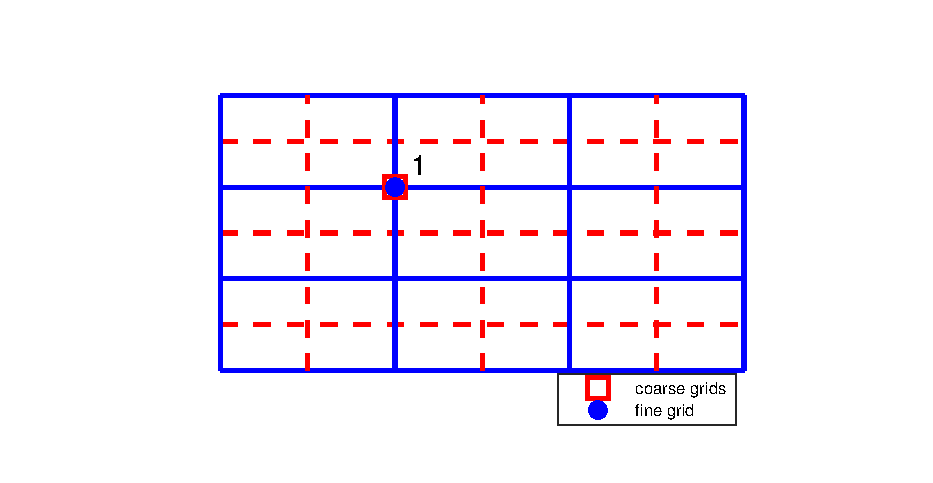
\includegraphics[width=0.45\textwidth]{interpolation1.eps}
	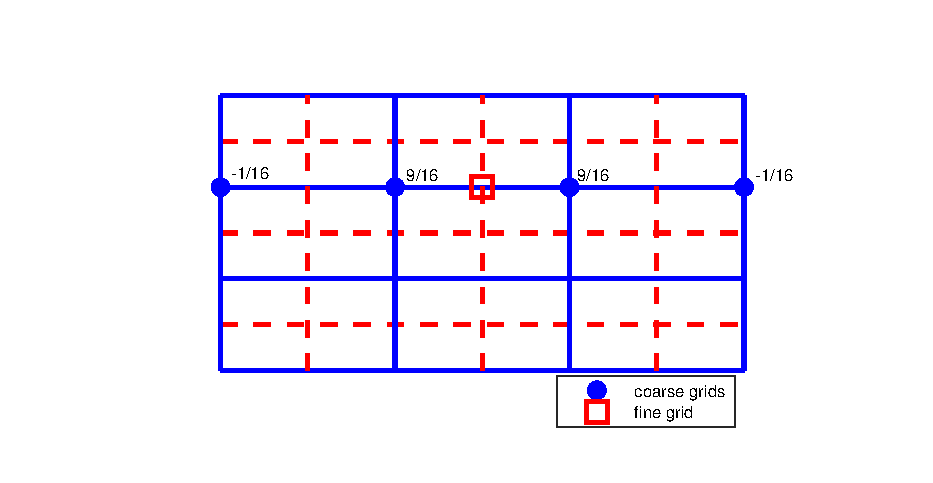
\includegraphics[width=0.45\textwidth]{interpolation2.eps}
	\caption{\scriptsize{From left to right, the sketch of interpolation stencil for $(i_1^f,i_2^f) =$ (odd, odd) and $(i_1^f,i_2^f) =$ (even, odd) respectively. The number at the right-top corner are the coefficients of the corresponding coarse grids.}}\label{interpolation_1_2}
\end{figure}
Figure \ref{interpolation_1_2} illustrates the interpolation coefficients when $(i_1^f,i_2^f) = $ (odd, odd) and  $(i_1^f,i_2^f) = $ (even, odd) respectively. While Figure \ref{interpolation_3_4} gives the interpolation coefficients when $(i_1^f,i_2^f) = $ (odd, even) and  $(i_1^f,i_2^f) = $ (even, even) respectively.
\begin{figure}[H]
	\centering
	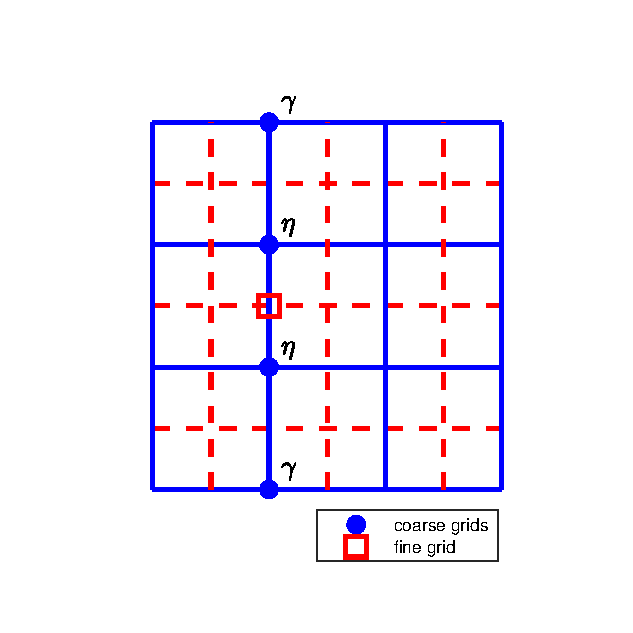
\includegraphics[width=0.45\textwidth]{interpolation3.eps}
	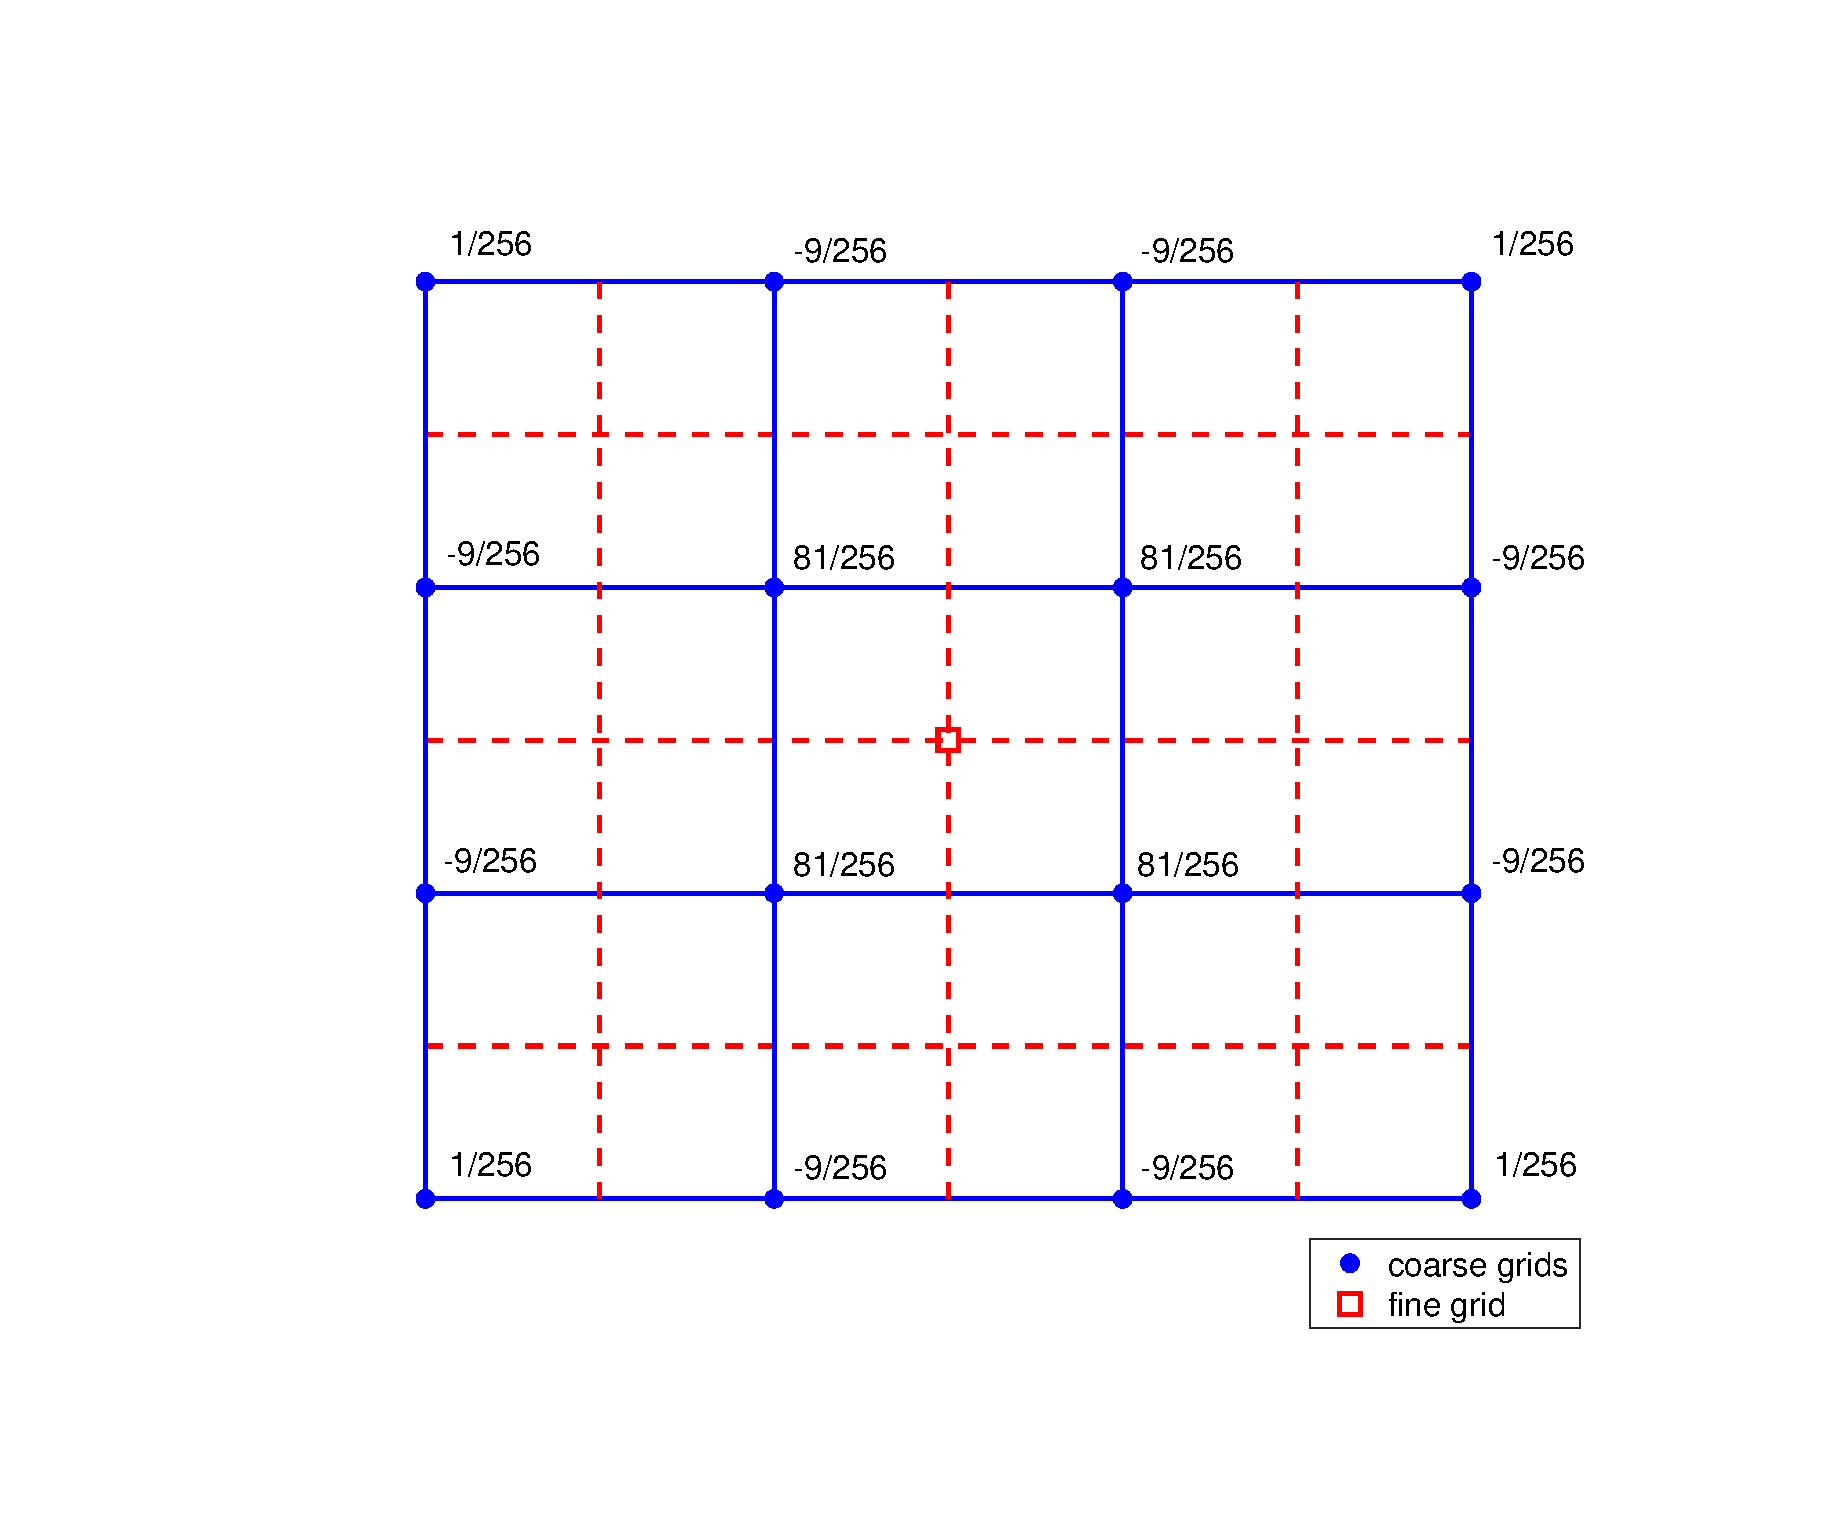
\includegraphics[width=0.45\textwidth]{interpolation4.eps}
	\caption{\scriptsize{From left to right, the sketch of interpolation stencil for $(i_1^f,i_2^f) =$ (odd, even) and $(i_1^f,i_2^f) =$ (even, even) respectively. The number at the right-top corner are the coefficients of the corresponding coarse grids.}}\label{interpolation_3_4}
\end{figure}

Furthermore, the compatibility condition of the intrpolation operator $\mathcal{P}$ and restriction operator $\mathcal{R}$, $\mathcal{P} = 4\mathcal{R}^T$ for $h_1^c = 2h_1^f$ in $2$D, determines the corresponding restriction operator $\mathcal{R}$ with
\begin{equation}\label{restriction}
({\bf u}^c|_{\Gamma})_{i^c,j^c} = (\mathcal{R}{\bf u}^f|_{\Gamma})_{i^c,j^c} = \mathcal{A}^2\mathcal{A}^1 ({\bf u}^f|_{\Gamma})_{2i^c-1,2j^c-1},
\end{equation}
where $\mathcal{A}^j, j = 1,2$ are the fourth order restriction operators in $1$D for the direction $j$. Figure \ref{extrapolation} shows the restriction coefficients for the coarse grids $(i_1^c,i_2^c)$.

\begin{figure}[H]
	\centering
	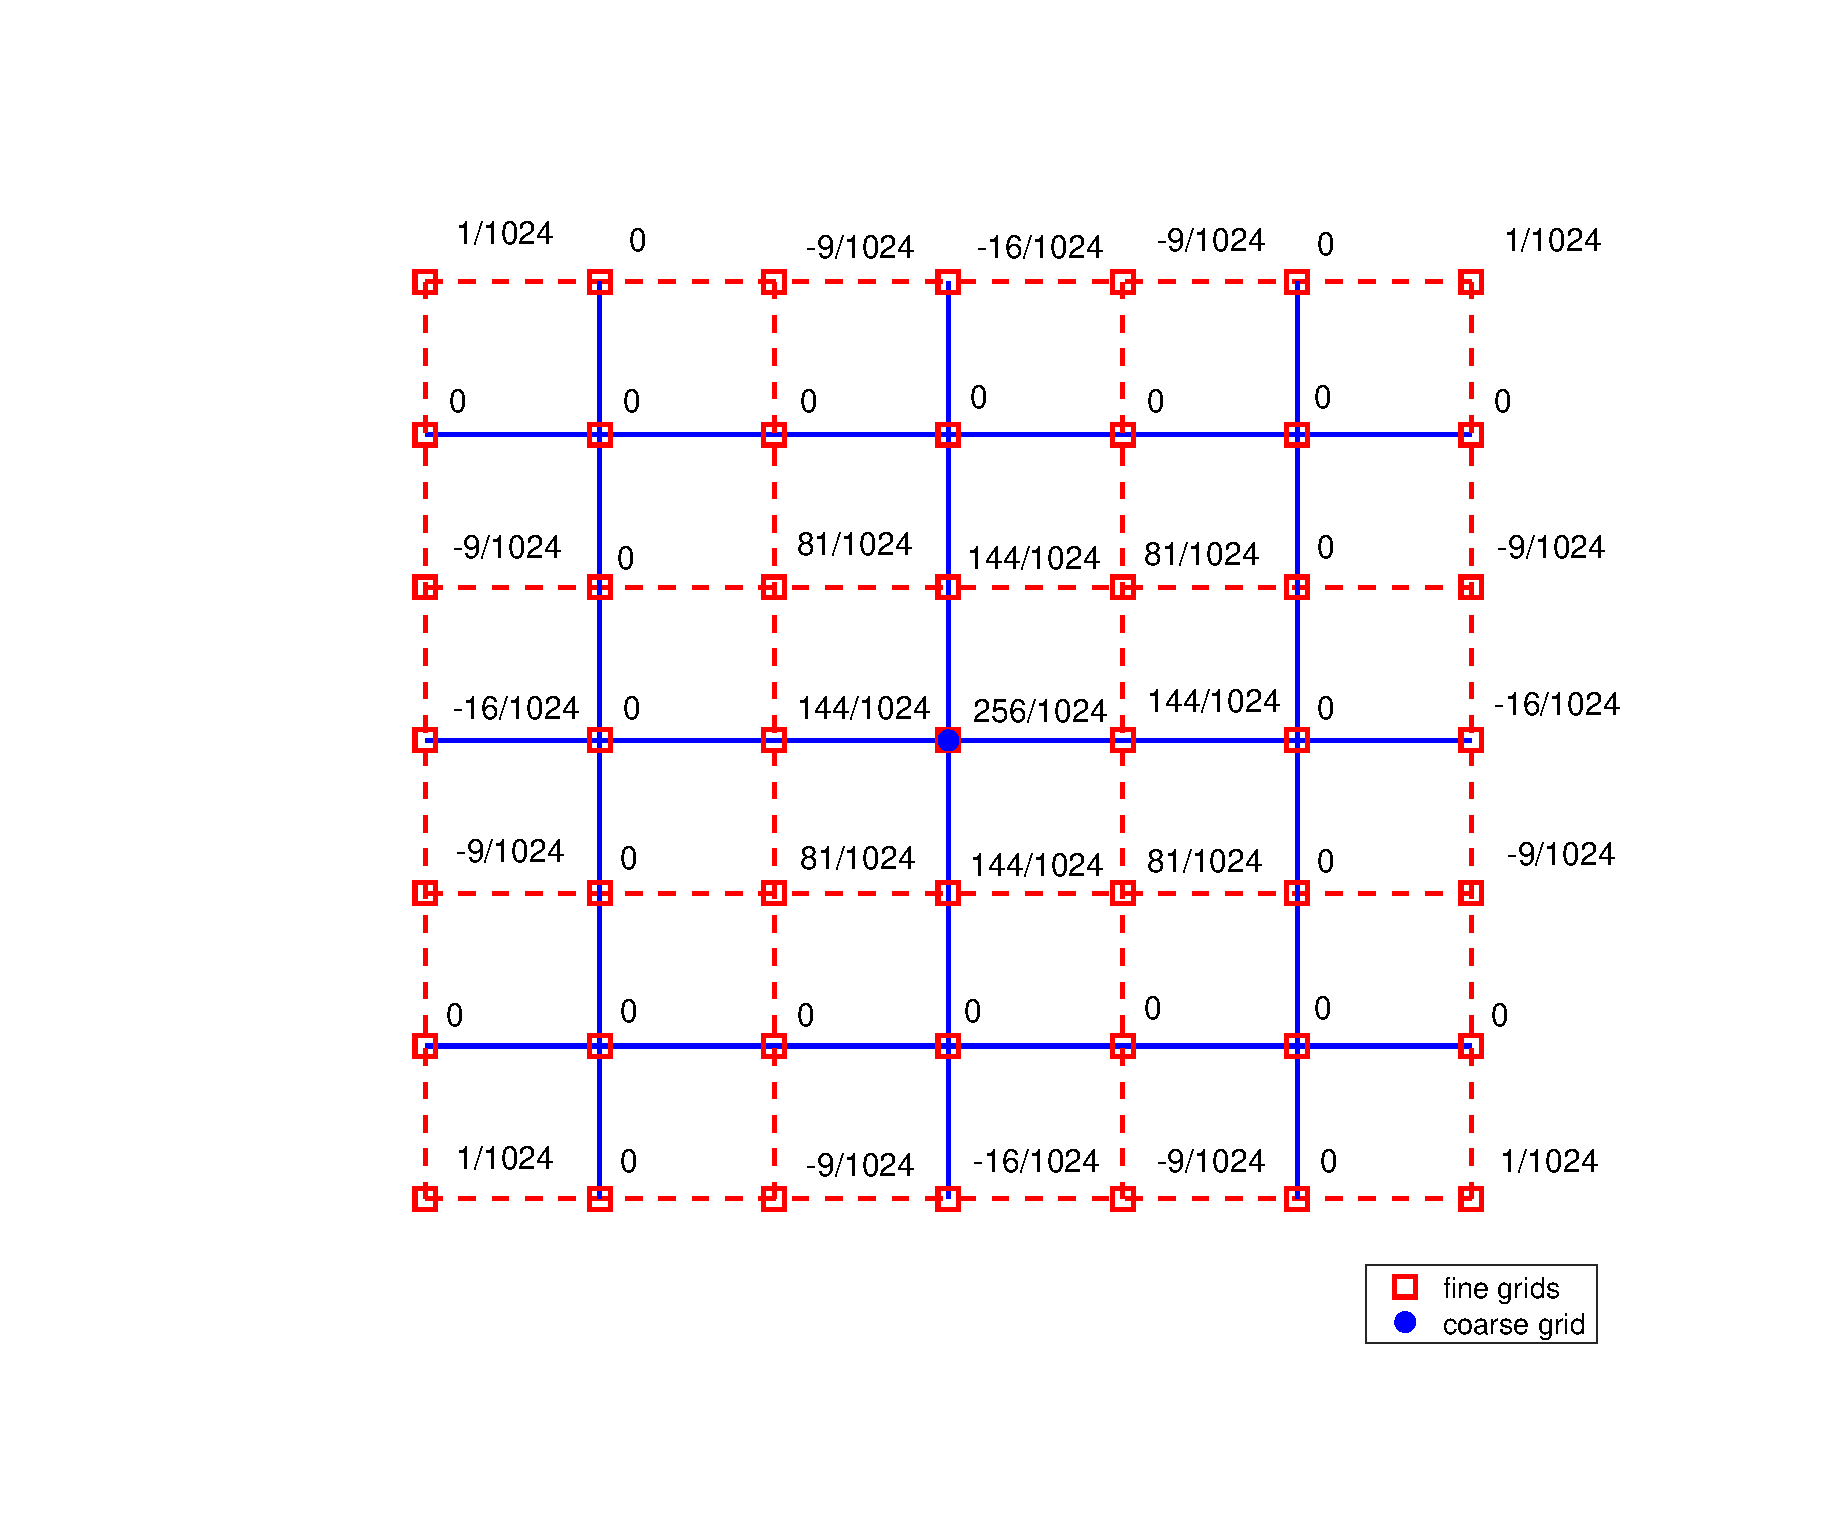
\includegraphics[width=0.8\textwidth]{extrapolation.eps}
	\caption{\scriptsize{The sketch of extrapolation stencil in $2$D. The number at the right-top corner are the coefficients of the corresponding fine grids.}}\label{extrapolation}
\end{figure}
 For the simplicity of analysis, we introduce a general notation for the schemes (\ref{fine_scheme_2}) and (\ref{fine_scheme_1}) in the fine domain $\Omega_f$,
\begin{align}\label{fine_scheme}
\rho^f_{{\bf i}^f} ({\bf u}_{tt}^f)_{{\bf i}^f} = \hat{L}_{h^f}{\bf u}^f_{{\bf i}^f} =  \left\{
\begin{aligned}
&\wt{L}_{h^f}{\bf{u}}^f_{{\bf i}^f}, \ \ i_3^f = 2,3,\cdots,n_3^f,\\
&L_{h^f}{\bf u}^f_{{\bf i}^f_{\Gamma}}+{\bm \eta}_{i^f,j^f}/J^f_{{\bf i}^f_{\Gamma}},
\end{aligned}
\right.
\end{align}
For the grids in the fine domain $\Omega^f$  that are lying on the interface $\Gamma$, we impose the continuity of the solution,
\begin{equation}\label{data_continuous_curvi}
{\bf u}^f\big|_{\Gamma} = \mathcal{P}\big({\bf u}^c\big|_{\Gamma}\big).
\end{equation}
As for the ghost points which are close to the top surface of the coarse domian, we impose the continuity of the traction force,
\begin{equation}\label{traction_continuous_curvi}
{\bf n}^c\cdot\mathcal{T}^c \big|_\Gamma = \mathcal{R}\left(-{\bf n}^f\cdot\mathcal{T}^f\big|_\Gamma - \frac{h_3^f\omega_1^{(3)}{\bm \eta}}{J^f\big|\nabla r_f^{(3)}\big|}\Bigg|_\Gamma\right).
\end{equation}

\subsection{Energy estimate}
%We derive an energy estimate, which tells us what interface conditions we shall impose. Also discuss boundary conditions. Be careful with the Jacobian.

%These two sections should not be too long. We shall cite previous works by Petersson and Sjögreen, and also Duru and Virta 2014. 

In this section, we investigate the energy estimate for the semi-discrete form of the SBP scheme in section \ref{sub_section_4_1}. Define the discrete scalar product on the interface surface $\Gamma$ by,
\begin{equation}\label{scalar_product_discrete_interface_c}
({\bf u}^c, {\bf v}^c)_{h^c,\Gamma} = h_1^ch_2^c\sum_{i_1^c=1}^{n_1^c}\sum_{i_2^c=1}^{n_2^c}\omega_{i_1^c}^{(1)}\omega_{i_2^c}^{(2)}\left(J^c\big|\nabla r^{3}\big|\right)_{{\bf i}^c_{\Gamma}}({\bf u}^c_{{\bf i}^c_{\Gamma}})^T{\bf v}_{{\bf i}^c_{\Gamma}}^c,
\end{equation}
for coarse domain $\Omega^c$ and
\begin{equation}\label{scalar_product_discrete_interface_f}
({\bf u}^f, {\bf v}^f)_{h^f,\Gamma} = h_1^fh_2^f\sum_{i_1^f=1}^{n_1^f}\sum_{i_2^f=1}^{n_2^f}\omega_{i_1^f}^{(1)}\omega_{i_2^f}^{(2)}\left(J^f\big|\nabla r^{3}\big|\right)_{{\bf i}^f_{\Gamma}}({\bf u}^f_{{\bf i}^f_{\Gamma}})^T{\bf v}_{{\bf i}^f_{\Gamma}}^f,
\end{equation}
for fine domain $\Omega^f$. Multiplying (\ref{coarse_scheme}) by $h_1^ch_2^ch_3^c\omega_{i_1^c}^{(1)}\omega_{i_2^c}^{(2)}\omega_{i_3^c}^{(3)}J_{{\bf i}^c}^c$ and summing over all grids, we have
\begin{equation}\label{coarse_simple}
({\bf u}_t^c, \rho^c{\bf u}_{tt}^c)_{h^c} = -S_{h^c}({\bf u}_t^c,{\bf u}^c) + B_{h^c}({\bf u}_t^c,{\bf u}^c),
\end{equation}
multiplying (\ref{fine_scheme_1}) by $h_1^fh_2^fh_3^f\omega_{i_1^f}^{(1)}\omega_{i_2^f}^{(2)}\omega_{i_3^f}^{(3)}J_{{\bf i}^f}^f$ and summing over all grids, we obtain
\begin{multline}\label{fine_simple}
({\bf u}_t^f, \rho^f{\bf u}_{tt}^f)_{h^f} = -S_{h^f}({\bf u}_t^f,{\bf u}^f) + B_{h^f}({\bf u}_t^f,{\bf u}^f) \\
+h_3^f\omega_1^{(3)}h_1^fh_2^f\sum_{i_1^f=1}^{n_1^f}\sum_{i_2^f=1}^{n_2^f}\omega_{i_1^f}^{(1)}\omega_{i_2^f}^{(2)}({\bf u}_t^f)_{{\bf i}^f_{\Gamma}}^{T}{\bm \eta}_{i_1^f,i_2^f},
\end{multline}
where  $S_{h^c}$ and $S_{h^f}$ can be found in Appendix ?, and 
\begin{equation}\label{boundary_f}
B_{h^f} ({\bf u}_t^f,{\bf u}^f) = -h_1^fh_2^f\sum_{i_1^f = 1}^{n_1^f}\sum_{i_2^f=1}^{n_2^f}\omega_{i_1^f}^{(1)}\omega_{i_2^f}^{(2)}({\bf u}_t^f)^T_{{\bf i}^f_{\Gamma}}\big(N_{31}^fD_1^f {\bf u}^f_{{\bf i}^f_{\Gamma}}+ N_{32}^fD_2^f{\bf u}^f_{{\bf i}^f_{\Gamma}}+N_{33}^fD_3^f{\bf u}^f_{{\bf i}^f_{\Gamma}}\big),
\end{equation}
and
\begin{equation}\label{bounary_c}
B_{h^c} ({\bf u}_t^c,{\bf u}^c) = h_1^ch_2^c\sum_{i_1^c = 1}^{ n_1^c}\sum_{i_2^c=1}^{n_2^c}\omega_{i_1^c}^{(1)}\omega_{i_2^c}^{(2)}({\bf u}_t^f)^T_{{\bf i}^c_{\Gamma}}\big(N_{31}^cD_1^c {\bf u}^c_{{\bf i}^c_{\Gamma}}+ N_{32}^cD_2^c{\bf u}^c_{{\bf i}^c_{\Gamma}}+N_{33}^c\wt{D}_3^c{\bf u}^c_{{\bf i}^c_{\Gamma}}\big),
\end{equation}
provided periodic boundary conditions in the directions $1$ and $2$, a homogeneous Dirichlet boundary condition on the bottom surface and a free surface boundary condition on the top surface. Finally, we conclude a time derivative of the semi-discrete energy
\begin{multline}\label{semi_energy_1}
\frac{d}{dt}\big[({\bf u}_t^f,\rho^f {\bf u}_t^f)_{h^f} + S_{h^f}({\bf u}^f,{\bf u}^f_t) + ({\bf u}_t^c,\rho^c {\bf u}_t^c)_{h^c} + S_{h^c}({\bf u}^c,{\bf u}^c_t) \big]  = \\
2B_{h^f}({\bf u}_t^f,{\bf u}^f) + 2B_{h^c}({\bf u}_t^c,{\bf u}^c) + 2h_3^f\omega_1^{(3)}h_1^f h_2^f\sum_{i_1^f=1}^{n_1^f}\sum_{i_2^f=1}^{n_2^f}\omega_{i_1^f}^{(1)}\omega_{i_2^f}^{(2)}({\bf u}_t^f)^T_{{\bf i}^f_{\Gamma}}{\bm \eta}_{i_1^f,i_2^f},
\end{multline}
plugging (\ref{boundary_f}) and (\ref{bounary_c}) into (\ref{semi_energy_1}) and combining the definition of the scalar product on the interface $\Gamma$ (\ref{scalar_product_discrete_interface_c}) and (\ref{scalar_product_discrete_interface_f}), we have
\begin{multline}\label{semi_energy_2}
\frac{d}{dt}\left[({\bf u}_t^f,\rho^f {\bf u}_t^f)_{h^f} + S_{h^f}({\bf u}^f,{\bf u}^f_t) + ({\bf u}_t^c,\rho^c {\bf u}_t^c)_{h^c} + S_{h^c}({\bf u}^c,{\bf u}^c_t) \right]  = \\
2\left(-{\bf u}_t^f,\frac{\hat{A}_3^f{\bf u}^f}{J^f|\nabla r_f^{(3)}|}\right)_{h_f,\Gamma} + 2\left({\bf u}_t^c,\frac{\hat{A}_3^c{\bf u}^c}{J^c|\nabla r_c^{(3)}|}\right)_{h_c,\Gamma} + 2\left({\bf u}_t^f,\frac{h_3^f\omega_1^{(3)}{\bm \eta}}{J^f|\nabla r_f^{(3)}|}\right)_{h_f,\Gamma} = \\
2\left({\bf u}_t^f,-\frac{\hat{A}_3^f{\bf u}^f}{J^f|\nabla r_f^{(3)}|} + \frac{h_3^f\omega_1^{(3)}{\bm \eta}}{J^f|\nabla r_f^{(3)}|}\right)_{h_f,\Gamma} +  2\left({\bf u}_t^c,\frac{\hat{A}_3^c{\bf u}^c}{J^c|\nabla r_c^{(3)}|}\right)_{h_c,\Gamma} = \\
2\left(\mathcal{P}{\bf u}^c_t,-\frac{\hat{A}_3^f{\bf u}^f}{J^f|\nabla r_f^{(3)}|} + \frac{h_3^f\omega_1^{(3)}{\bm \eta}}{J^f|\nabla r_f^{(3)}|}\right)_{h_f,\Gamma} + 2\left({\bf u}_t^c,\frac{\hat{A}_3^c{\bf u}^c}{J^c|\nabla r_c^{(3)}|}\right)_{h_c,\Gamma} = \\
2\left({\bf u}_t^c,\mathcal{R}\Big(-\frac{\hat{A}_3^f{\bf u}^f}{J^f|\nabla r_f^{(3)}|} + \frac{h_3^f\omega_1^{(3)}{\bm \eta}}{J^f|\nabla r_f^{(3)}|}\Big)\right)_{h_c,\Gamma} + 2\left({\bf u}_t^c,\frac{\hat{A}_3^c{\bf u}^c}{J^c|\nabla r_c^{(3)}|}\right)_{h_c,\Gamma}.
\end{multline}
Here, to simplify the formula,  we have used the notations
\begin{equation}\label{hatAf}
\hat{A}_3^f{\bf u}^f_{{\bf i}^f} = N^f_{31}D^f_1{\bf u}^f_{{\bf i}^f} + N^f_{32}D^f_2{\bf u}^f_{{\bf i}^f} + N^f_{33}D^f_3{\bf u}^f_{{\bf i}^f},
\end{equation}
and
\begin{equation}\label{hatAc}
\hat{A}_3^c{\bf u}^c_{{\bf i}^c} = N^c_{31}D^c_1{\bf u}^c_{{\bf i}^c} + N^c_{32}D^c_2{\bf u}^c_{{\bf i}^c} + N^c_{33}\wt{D}^c_3{\bf u}^c_{{\bf i}^c}.
\end{equation}
Sine we have the fact (\ref{traction_continuous_curvi}) in the cuvilinear coordinates, then combine with (\ref{bdry3_curvi}) arrives at
\begin{equation*}
\frac{\hat{A}_3^c{\bf u}^c}{J^c|\nabla r_c^{(3)}|}\Bigg|_{\Gamma} = \mathcal{R}\left(\frac{\hat{A}_3^f{\bf u}^f}{J^f|\nabla r_f^{(3)}|}\Bigg|_{\Gamma} - \frac{h_3^f\omega_1^{(3)}{\bm \eta}}{J^f|\nabla r_f^{(3)}|}\Bigg|_{\Gamma}\right),
\end{equation*}
finally, we conclude that
\begin{equation*}
\frac{d}{dt}\left[({\bf u}_t^f,\rho^f {\bf u}_t^f)_{h^f} + S_{h^f}({\bf u}^f,{\bf u}^f_t) + ({\bf u}_t^c,\rho^c {\bf u}_t^c)_{h^c} + S_{h^c}({\bf u}^c,{\bf u}^c_t) \right]  = 0
\end{equation*}
without external force.

\section{The temporal discretization}
%We present the predictor-corrector discretization in time, and explain how the ghost points are updated. In addtion, we describle the iterative methods. Perhaps we shall also talk about CFL and the time steps. Maybe no fully-discrete energy analysis? That would be very messy. 
The equations are advanced in time with an explicit fourth order accurate predictor-corrector time integration method. Like all explicit time stepping methods, there is a maximum time step not exceed CFL stabilitity limit.

In \cite{?}, it is proved that the time step constraint by CFL condition for the Newmark scheme 
\begin{equation*}
\frac{{\bf u}^{n+1}-2{\bf u}^n + {\bf u}^{n-1}}{\Delta_t^2} = {\bf L}_h{\bf u}^n + {\bf F}^n, \ \ \ n = 0,1,\cdots
\end{equation*}
 which is second order if
\begin{equation*}
\frac{\Delta_t^2}{h^2}\kappa_{\text{max}}\leq C_{\text{cfl}}^2.
\end{equation*}
Here, 
$\kappa_{\text{max}}$ is the maximum of the eigenvalue of the matrix 
\[T = \frac{1}{\rho}\left(\begin{array}{ccc}
Tr(N_{11}) &  Tr(N_{12})& Tr(N_{13})\\
Tr(N_{21}) & Tr(N_{22}) & Tr(N_{23})\\
Tr(N_{31}) & Tr(N_{32}) & Tr(N_{33})\end{array}\right). \]
Here, $Tr(N_{ij})$ represents the trace of the matrix $N_{ij},i,j = 1,2,3$. In this paper, we use the predictor-corrector strategy to obtain a fourth order time integrator. In \cite{?}, it shows that the fourth order scheme has a somewhat larger stability limit for the time step, but the way used to approximate eigenvalue is same. We use $C_{\text{cfl}} = 1.9$ in the numrical experiments in this paper.

\subsection{Time discretization with SBP scheme}
In the following, we give the detailed procedures about how we apply the fourth order time integrator to the problem (\ref{coarse_scheme}) -- (\ref{traction_continuous_curvi}). 

Let ${\bf u}^{n,c}$ and ${\bf u}^{n,f}$ denote the numerical approximations of ${\bf u}({\bf x},t_n), {\bf x}\in\Omega_c$ and ${\bf u}({\bf x},t_n), {\bf x}\in\Omega_f$ respectively. Here, $t_n = n\Delta t, n = 0,1,\cdots$ and $\Delta_t > 0$ is a constant time step. We present the fourth order time integrator with predictor and corrector in the Algorithm \ref{first_alg}.

\begin{breakablealgorithm}
	\caption{Fourth order accurate time steping for the elastic wave equation with SBP discretization in space}\label{first_alg}
	Given initial conditions $\uline{\wt{{\bf u}}}^{0,c}, \uline{\wt{{\bf u}}}^{-1,c}$ and $\wt{{\bf u}}^{0,f}, \wt{{\bf u}}^{-1,f}$ that satisfies the discretized boundary conditions.
	
	\begin{itemize}
	\item  {Compute the predictor at the interior grid points for both fine and coarse domains {\color{red}(We use L instead of E, right?)}
		\begin{equation*}
		   {\bf u}^{c,*,n+1}_{{\bf i}^c} = 2{\bf u}^{c,n}_{{\bf i}^c} - {\bf u}^{c,n-1}_{{\bf i}^c} + \Delta_t^2(\rho^c_{{\bf i}^c})^{-1}\uline{\wt{E}}_c(\mu_{{\bf i}^c},\lambda_{{\bf i}^c}) {\bf{u}}^{c,n}_{{\bf i}^c}
		\end{equation*}
		\begin{equation*}
		{\bf u}^{f,*,n+1}_{{\bf i}^f} = 2{\bf u}^{f,n}_{{\bf i}^f} - {\bf u}^{f,n-1}_{{\bf i}^f} + \Delta_t^2(\rho^f_{{\bf i}^f})^{-1}{\wt{E}}_f(\mu_{{\bf i}^f},\lambda_{{\bf i}^f}) {\bf{u}}^{f,n}_{{\bf i}^f}
		\end{equation*}
	   }
   \item {For the boundary forcing condition, assign the ghost point value ${\bf u}^{f,*,n+1}_{i_1^f,i_2^f,n^f_3+1}$ to satisfy
   	\begin{equation*}
   	N_{31}^fD_1{\bf u}^{f,*,n+1}_{{\bf i}^f_{\Omega^f_t}} + N_{32}^fD_2{\bf u}^{f,*,n+1}_{{\bf i}^f_{\Omega^f_t}} + N_{33}^fD_3{\bf u}^{f,*,n+1}_{{\bf i}^f_{\Omega^f_t}} = {\bf g}_{i_1^f,i_2^f}(t_{n+1})(J^f|\nabla r^{(3)}|)_{{\bf i}^f_{\Omega^f_t}}
   	\end{equation*}
   }
   \item {For the Dirichlet boundary condition, assign the ghost point value ${\bf u}^{c,*,n+1}_{i_1^c,i_2^c,0}$ to satisfy
   	\begin{equation*}
   	\uline{\wt{M}}_c(\mu_{{\bf i}^c_{\Omega^c_b}},\lambda_{{\bf i}^c_{\Omega^c_b}}) {\bf{u}}^{c,*,n+1}_{{\bf i}^c_{\Omega^c_b}} = 2\uline{\wt{M}}_c(\mu_{{\bf i}^c_{\Omega^c_b}},\lambda_{{\bf i}^c_{\Omega^c_b}}) {\bf{u}}^{c,*,n}_{{\bf i}^c_{\Omega^c_b}} - 	\uline{\wt{M}}_c(\mu_{{\bf i}^c_{\Omega^c_b}},\lambda_{{\bf i}^c_{\Omega^c_b}}) {\bf{u}}^{c,*,n-1}_{{\bf i}^c_{\Omega^c_b}}
   	\end{equation*}
   }
  \item{For the continuity of solution on the interface $\Gamma$, assign the value ${\bf u}^{f,*,n+1}_{i_1^f,i_2^f,0}$ to satisfy
  	\begin{equation*}
  	{\bf u}^{f,*,n+1}\big|_{\Gamma} = \mathcal{P}\big({\bf u}^{c,*,n+1}\big|_{\Gamma}\big)
  	\end{equation*}
  }
  \item{For the continuity of traction force on the interface $\Gamma$, assign the ghost point value ${\bf u}^{c,*,n+1}_{i_1^c,i_2^c,n_3^c+1}$ to satisfy
  	\begin{equation}\label{traction_gamma_pre}
  	\frac{\hat{A}_3^c{\bf u}^{c,*,n+1}}{J^c|\nabla r_c^{(3)}|}\Bigg|_{\Gamma} = \mathcal{R}\left(\frac{\hat{A}_3^f{\bf u}^{f,*,n+1}}{J^f|\nabla r_f^{(3)}|}\Bigg|_{\Gamma} - \frac{h_3^f\omega_1^{(3)}{\bm \eta}^*}{J^f|\nabla r_f^{(3)}|}\Bigg|_{\Gamma}\right)
  	\end{equation}
  	with the definition of $\hat{A}^c_3$ in (\ref{hatAc}), $\hat{A}^f_3$ in (\ref{hatAf}) and ${\bm \eta}^*$ has a similar definition as in (\ref{eta}) with ${\bf u}$ substituted by ${\bf u}^*$
  }
  \item{Evaluate the acceleration at all grids 
  	\begin{equation*}
  	\uline{\wt{\bf v}}^{c,n} = \frac{\uline{\wt{\bf u}}^{c,*,n+1}-2\uline{\wt{\bf u}}^{c,n}+\uline{\wt{\bf u}}^{c,n-1}}{\Delta^2_t}
  	\end{equation*}
  	\begin{equation*}
  	\wt{\bf v}^{f,n} = \frac{\wt{\bf u}^{f,*,n+1}-2\wt{\bf u}^{f,n}+\wt{\bf u}^{f,n-1}}{\Delta^2_t}
  	\end{equation*}
  }
  \item{Compute the corrector at the interior grid points
  	\begin{equation*}
  	{\bf u}^{c,n+1}_{{\bf i}^c} = {\bf u}^{c,*,n+1}_{{\bf i}^c} + \frac{\Delta_t^4}{12}(\rho^c_{{\bf i}^c})^{-1}\uline{\wt{E}}_c(\mu_{{\bf i}^c},\lambda_{{\bf i}^c}) {\bf{u}}^{c,*,n}_{{\bf i}^c}
  	\end{equation*}
  	\begin{equation*}
  		{\bf u}^{f,n+1}_{{\bf i}^f} = {\bf u}^{f,*,n+1}_{{\bf i}^f} + \frac{\Delta_t^4}{12}(\rho^f_{{\bf i}^f})^{-1}\wt{E}_f(\mu_{{\bf i}^f},\lambda_{{\bf i}^f}) {\bf{u}}^{f,*,n}_{{\bf i}^f}
  	\end{equation*}
  }
 \item {For the boundary forcing condition, assign the ghost point value ${\bf u}^{f,n+1}_{i^f_1,i^f_2,n_3^f+1}$ to satisfy
 		\begin{equation*}
 	N_{31}^fD_1{\bf u}^{f,n+1}_{{\bf i}^f_{\Omega^f_t}} + N_{32}^fD_2{\bf u}^{f,n+1}_{{\bf i}^f_{\Omega^f_t}} + N_{33}^fD_3{\bf u}^{f,n+1}_{{\bf i}^f_{\Omega^f_t}} = {\bf g}_{i^c_1,i^c_2}(t_{n+1})(J^f|\nabla r^{(3)}|)_{{\bf i}^f_{\Omega^f_t}}
 	\end{equation*}	
 }
 \item {For the Dirichlet boundary condition, assign the ghost point value ${\bf u}^{c,n+1}_{i^c_1,i^c_2,0}$ to satify
 	\begin{equation*}
 	\uline{\wt{M}}(\mu_{{\bf i}^c_{\Omega^c_b}},\lambda_{{\bf i}^c_{\Omega^c_b}}){\bf u}_{{\bf i}^c_{\Omega^c_b}}^{c,n+1} = \frac{\rho^c_{{\bf i}^c_{\Omega^c_b}}}{\Delta_t^2}\Big({\bf f} _{i^c_1,i^c_2}(t_{n+2})-2{\bf u}_{{\bf i}^c_{\Omega^c_b}}^{c,n+1}+{\bf u}_{{\bf i}^c_{\Omega^c_b}}^{c,n}\Big)
 	\end{equation*}
 }
 \item{For continuity of solution on the interface $\Gamma$, assign the value ${\bf u}^{f,n+1}_{i^c_1,i^c_2,0}$ to satisfy
	\begin{equation*}
	{\bf u}^{f,n+1}\big|_{\Gamma} = \mathcal{P}\big({\bf u}^{c,n+1}\big|_{\Gamma}\big)
	\end{equation*}
}
\item{For the continuity of traction force on the interface $\Gamma$, assign the ghost point value ${\bf u}^{c,n+1}_{i,j,n_3^c+1}$ to satisfy
	\begin{equation}\label{traction_gamma_corr}
	\frac{\hat{A}_3^c{\bf u}^{c,n+1}}{J^c|\nabla r_c^{(3)}|}\Bigg|_{\Gamma} = \mathcal{R}\left(\frac{\hat{A}_3^f{\bf u}^{f,n+1}}{J^f|\nabla r_f^{(3)}|}\Bigg|_{\Gamma} - \frac{h_3^f\omega_1^{(3)}{\bm \eta}}{J^f|\nabla r_f^{(3)}|}\Bigg|_{\Gamma}\right)
	\end{equation}
	with the definition of $\hat{A}^c_3$ in (\ref{hatAc}), $\hat{A}^f_3$ in (\ref{hatAf}) and ${\bm \eta}$ in (\ref{eta})
}
	\end{itemize}
\end{breakablealgorithm}
Here, we only give the steps to evolve the elatic wave equation with suitable initial and boundary condiitons and skip the detailed derivations of the fourth order predictor corrector time integator. One can refer to \cite{?} to get more details.

In the Algorithm \ref{first_alg}, we need to solve the equations come from the continuity of the traction force for the interface $\Gamma$ in both preditor step (\ref{traction_gamma_pre}) and corrector step (
\ref{traction_gamma_corr}). The structure of (\ref{traction_gamma_pre}) and (\ref{traction_gamma_corr}) are same, for simplicity, we only clarify how we solve (\ref{traction_gamma_pre}) in the predictor step.

Note that there are $3n_1^cn_2^c$ unknowns in (\ref{traction_gamma_pre}) and $3n_1^cn_2^c$ linear equations in (\ref{traction_gamma_pre}). Since it is very expensive to calculate the LU-factorization for a large problem in $3$D and there is no efficient ways to calculate the LU-factorization in a parallel machine, we instead using iterative methods to solve the linear system (\ref{traction_gamma_pre}). Specificly, we use three different iterative methods: block Jacobian iterative method, conjugate gradient iterative method, pre-conditioned conjugate gradient iterative method, to solve (\ref{traction_gamma_pre}). The details are given in Section \ref{iterative_section}.

\section{Numerical Experiments}
In this section, we conduct several numerical experiments. In Section \ref{manufactured_sol}, we compare the efficiency of iterative methods which are used to solve the interface condition system (\ref{traction_gamma_pre}) and (\ref{traction_gamma_corr}), note that the coefficient matrices in (\ref{traction_gamma_pre}) and (\ref{traction_gamma_corr}) are same, verify the order of the convergence of the proposed scheme (\ref{coarse_scheme})--(\ref{traction_continuous_curvi}). In Section \ref{gaussian_source}, we show that there is no reflection at the mesh refinment interfaces for the proposed scheme (\ref{coarse_scheme})--(\ref{traction_continuous_curvi}) with only a traction force on the top surface. Finally, the energy conservation property is shown in Section \ref{conserved_energy}.
\subsection{Method of manufactured solutions}\label{manufactured_sol}
We take the computation domain to be 
\begin{equation}\label{coarse_domain_manufactured}
 \left\{
\begin{aligned}
& x^{c,(1)} = 2\pi r^{(1)}\\
& x^{c,(2)} = 2\pi r^{(2)}\\
& x^{c,(3)} = r^{(3)}\theta_i\big(r^{(1)},r^{(2)}\big) + (1-r^{(3)})\theta_b\big(r^{(1)},r^{(2)}\big)
\end{aligned}
\right.
\end{equation}
for coarse domain $\Omega_c$. Here, $0\leq r^{(1)}, r^{(2)}, r^{(3)}\leq 1$, $f_i$ is the interface surface geometry,
\begin{equation}\label{iterface_geometry}
\theta_i\big(r^{(1)},r^{(2)}\big) = \pi+0.2\sin(4\pi r^{(1)})+0.2\cos(4\pi r^{(2)}),
\end{equation}
and 
$\theta_b$ is the bottom surface geometry,
\begin{equation}\label{bottom_geometry}
\theta_b\big(r^{(1)},r^{(2)}\big) = 0.2\exp\left(-\frac{(r^{(1)}-0.6)^2}{0.04}\right)+0.2\exp\left(-\frac{(r^{(2)}-0.6)^2}{0.04}\right).
\end{equation}
As for the fine domian $\Omega_f$, it is choose to be
\begin{equation}\label{fine_domain_manufactured}
\left\{
\begin{aligned}
& x^{f,(1)} = 2\pi r^{(1)}\\
& x^{f,(2)} = 2\pi r^{(2)}\\
& x^{f,(3)} = r^{(3)}\theta_t\big(r^{(1)},r^{(2)}\big) + (1-r^{(3)})\theta_i\big(r^{(1)},r^{(2)}\big),
\end{aligned}
\right.
\end{equation}
where $0\leq r^{(1)}, r^{(2)}, r^{(3)}\leq 1$, $\theta_t$ is the top surface geometry,
\begin{equation}\label{top_geometry}
\theta_t\big(r^{(1)},r^{(2)}\big) = 0.2\exp\left(-\frac{(r^{(1)}-0.5)^2}{0.04}\right)+0.2\exp\left(-\frac{(r^{(2)}-0.5)^2}{0.04}\right),
\end{equation}
and $\theta_i$ is the interface geometry which is given in (\ref{iterface_geometry}). Note that the subdomian 
$\Omega_f$ is on the top of the subdomain $\Omega_c$. For both fine and coarse domians, let the density vary according to
\begin{equation}\label{density_function}
\rho(x^{(1)},x^{(2)},x^{(3)}) = 2 + \sin(x^{(1)}+0.3)\sin(x^{(2)}+0.3)\sin(x^{(3)}-0.2),
\end{equation}
and material parameters $\mu, \lambda$ satisfy
\begin{equation}\label{mu_function}
\mu(x^{(1)},x^{(2)},x^{(3)}) = 3 + \sin(3x^{(1)}+0.1)\sin(3x^{(2)}+0.1)\sin(x^{(3)}),
\end{equation}
and 
\begin{equation}\label{lambda_function}
\lambda(x^{(1)},x^{(2)},x^{(3)})  = 21+ \cos(x^{(1)}+0.1)\cos(x^{(2)}+0.1)\sin^2(3x^{(3)}),
\end{equation}
respectively. Besides, we impose a boundary forcing on the top surface and Dirichlet boundary conditions for the other boundaries. The internal forcing ${\bf F}$, top boundary forcing ${\bf g}$ and initial conditions are chosen such that ${\bf u} = (u_1,u_2,u_3)^T$ with
\begin{align*}
u_1 &= \cos(x^{(1)}+0.3)\sin(x^{(2)}+0.3)\sin(x^{(3)}+0.2)\cos(t^2),\\
u_2 &= \sin(x^{(1)}+0.3)\cos(x^{(2)}+0.3)\sin(x^{(3)}+0.2)\cos(t^2),\\
u_3 &= \sin(x^{(1)}+0.2)\sin(x^{(2)}+0.2)\cos(x^{(3)}+0.2)\sin(t).
\end{align*}
For example, for the boundary forcing on the top surface, we impose 
\begin{equation}\label{traction_force}
{\bf g} = (g_1,g_2,g_3)^T = \sum_{i=1}^3\left(\sum_{j = 1}^3 M_{ij}\frac{\partial{\bf u}}{\partial x^{(j)}}\right) n^{(i)},
\end{equation}
where, $n^{(i)}$ is the element of the unit outward normal ${\bf n} = (n^{(1)},n^{(2)},n^{(3)})$ for the top surface. 

\subsubsection{Iterative methods}\label{iterative_section}
In the proposed scheme (\ref{coarse_scheme})--(\ref{traction_continuous_curvi}), we need to solve a $3n_1^cn_2^c\times 3n_1^cn_2^c$ linear system at each time step twice for the continutiy of the traction force along the interface (\ref{traction_gamma_pre}) and (\ref{traction_gamma_corr}). Even ethough we can do LU factorization one time before the time loop start and reuse it at each time step, it is vergy expensive to do LU factorization for a large problem. Besides, consider solving real problems which are usually in large scale, we want to perform the computation on many processors on a parallel distributed memory machine, but it is not clear how to calculate the LU factorization of a matrix on many processors. 

In this paper, we propose three iterative methods: block Jacobian method, conjugate gradient method, preconditioned conjugate gradient method. We find that preconditioned conjugate gradient method is the most efficient one and conjugate gradient method needs most iteration numbers.

For the problem proposed in Section \ref{manufactured_sol}, the structure of the coefficient matrix of the linear system (\ref{traction_continuous_curvi}) is shown in Figure \ref{Mass_matrix} which is determined by the interplation operator $\mathcal{P}$ and restriction operator $\mathcal{R}$. We choose the red circles in the purple circles in Figure \ref{Mass_matrix} to be the block Jacobian matrix in block Jacobian iterative method and pre-conditioning matrix in conjugate gradient iterative method. We also set a absolute error tolerance $1e-7$ for each iterative method.

\begin{table}[htb]
	\begin{center}
		\begin{tabular}{|c|c c c|}
			\hline
			$h^c_k = 2h^f_k$   & ~~~~ CG ~~~~& Block Jacobian & Preconditioned CG  \\
			\hline
			$2\pi/24$ &37.76& 24.96& 4.07\\
			\hline
			$2\pi/48$ &38.61 & 25.38 & 2.88\\
			\hline 
			$2\pi/96$ &39.14 &25.43 & 2.55\\
			\hline
		\end{tabular}
	\end{center}
\caption{condition number of matrices in conjugate gradient method, block Jacobian method, preconditioned conjugate gradient method}\label{condition_number}
\end{table} 
Table \ref{condition_number} shows the condition number of the original coefficient matrix, the block Jacobian matrix and the coefficient matrix after applying pre-conditioner respectively. We observe that the condition number for preconditioned conjugate gradient method is smallest which is consistent with the results for iteration number of different iterative methods : there is around $44$ iterations for conjugate gradient method, $13$ iterations for block Jacobian method and $9$ iterations for preconditioned conjugate method.

\begin{figure}[H]
	\centering
	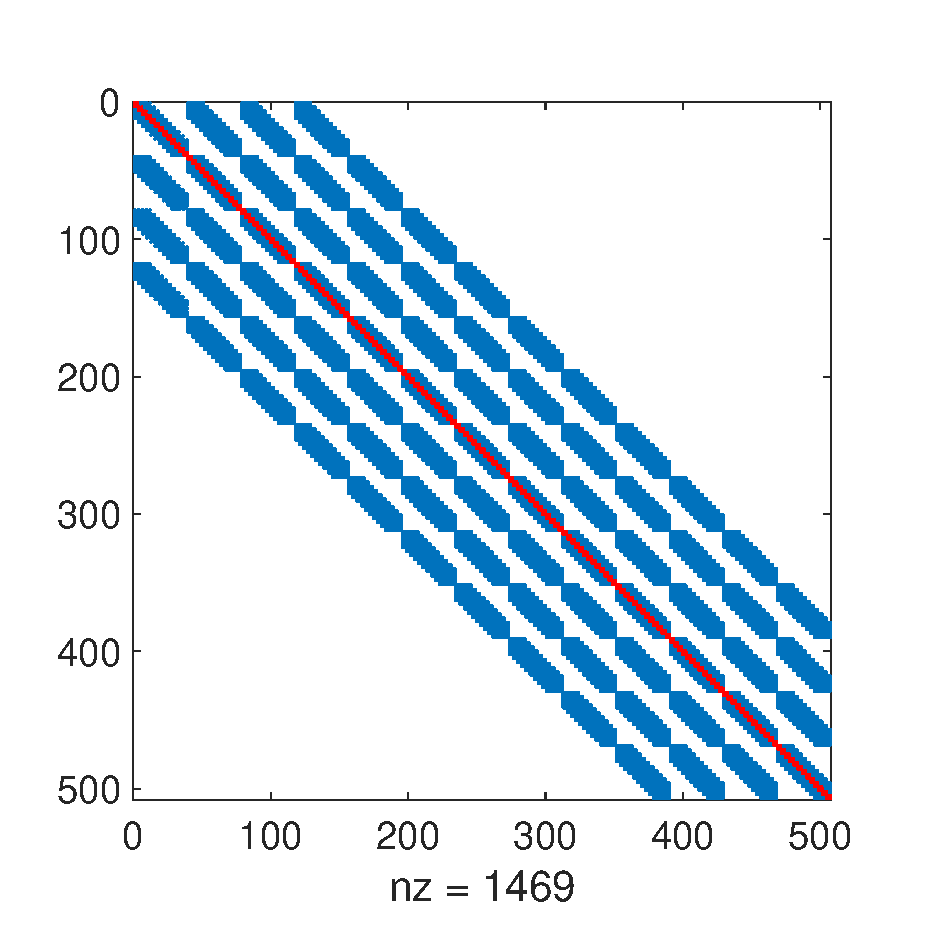
\includegraphics[width=0.45\textwidth]{Mass_matrix.eps}
	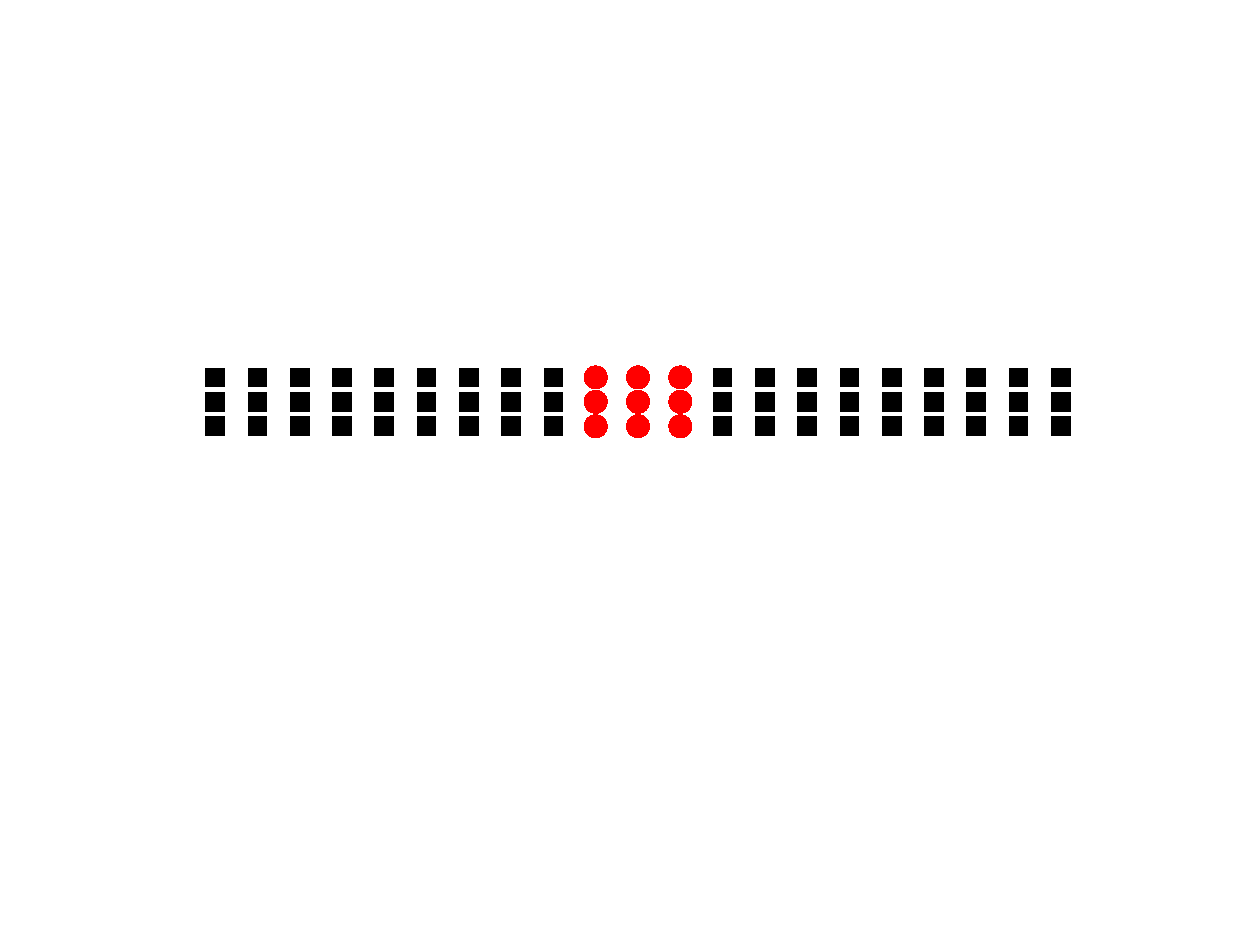
\includegraphics[width=0.45\textwidth]{Mass_block_diagonal.eps}
	\caption{\scriptsize{The left are the structure of the coefficient matrix of the linear system (\ref{traction_continuous_curvi}). For each triangle and circle in the left, it has the structure as in the right.}}\label{Mass_matrix}
\end{figure}

\subsubsection{Verification of convergence rate}\label{convergence_study}
We now perform a convergence study for the proposed scheme (\ref{coarse_scheme})--(\ref{traction_continuous_curvi}). The convergence rate is computed by
\[log\left(\frac{e_h}{e_{2h}}\right)\Bigg/log\left(\frac{1}{2}\right),\]
here, $e_h$ is the corresponding $L^2$ error.  The $L^2$ error for the numerical solutions in the whole domain, $L^{f,2}$ error for the numerical solutions in the fine domain $\Omega^f$ and$L^{c,2}$ error for the numerical solutions in the coarse domain $\Omega^c$ are presented in Table \ref{convergence_rate}. We observe that the convergence rate is fourth order for all cases, thought the theoretical convergence rate is second for the points near boundaries. Note that we use a block Jacobian iterative method for the experiments here.

\begin{table}[htb]
	\begin{center}
		\begin{tabular}{|c|c c c|}
			\hline
		    $h^c = 2h^f$   & $L^2$ & $L^{f,2}$ & $L^{c,2}$  \\
			\hline
			$2\pi/24$ &1.7740e-03 ~~~~~~~~ & 8.8534e-04 ~~~~~~~~ & 1.5373e-03 ~~~~~~~~\\
			\hline
			$2\pi/48$ &1.0658e-04 (4.06) & 5.5352e-05 (4.00) & 9.1084e-05 (4.08)\\
			\hline 
			$2\pi/96$ &6.3379e-06 (4.07) & 3.2694e-06 (4.08) & 5.4296e-06 (4.07)\\
			\hline
		\end{tabular}
	\end{center}
  \caption{Convergence rate of the fourth order SBP method}\label{convergence_rate}
\end{table} 

\subsection{Gaussian source}\label{gaussian_source}
%Show that no reflection at the mesh refinement interfaces. 
%If the code is incorporated into SW4, it would be nice to solve a practical problem. 
In this section, we present the numerical experiments to illustrate that there is no obvious artifacts are generated by the curvilinear interface. Specifically, we test the problem on the computation domain
\begin{equation}
\left\{
\begin{aligned}
& x^{c,(1)} = 2000 r^{(1)}\\
& x^{c,(2)} = 2000 r^{(2)}\\
& x^{c,(3)} = r^{(3)} \theta_i\big(r^{(1)},r^{(2)}\big) + (1-r^{(3)}) \theta_b\big(r^{(1)},r^{(2)}\big)
\end{aligned}
\right.
\end{equation}
for coarse domain $\Omega_c$. Here, $0\leq r^{(1)}, r^{(2)}, r^{(3)}\leq 1$, $\theta_i$ is the interface surface geometry,
\begin{equation}
\theta_i\big(r^{(1)},r^{(2)}\big) = 800+20\sin(4\pi r^{(1)})+20\cos(4\pi r^{(2)}),
\end{equation}
and 
$\theta_b$ is the bottom surface geometry,
\begin{equation}
\theta_b\big(r^{(1)},r^{(2)}\big) = 0.
\end{equation}
As for the fine domian $\Omega_f$, it is choose to be
\begin{equation}
\left\{
\begin{aligned}
& x^{f,(1)} = 2000 r^{(1)}\\
& x^{f,(2)} = 2000 r^{(2)}\\
& x^{f,(3)} = r^{(3)}\theta_t\big(r^{(1)},r^{(2)}\big) + (1-r^{(3)})\theta_i\big(r^{(1)},r^{(2)}\big),
\end{aligned}
\right.
\end{equation}
where $0\leq r^{(1)}, r^{(2)}, r^{(3)}\leq 1$, $\theta_t$ is the top surface geometry,
\begin{equation}
\theta_t\big(r^{(1)},r^{(2)}\big) = 1000,
\end{equation}
and $\theta_i$ is the interface geometry which is given in (\ref{iterface_geometry}). Note that the subdomian 
$\Omega_f$ is on the top of $\Omega_c$. For both fine and coarse domians, let the density vary according to
\begin{equation}
\rho(x^{(1)},x^{(2)},x^{(3)}) = 1.5\times 10^3,
\end{equation}
and material parameters $\mu, \lambda$ satisfy
\begin{equation}
\mu(x^{(1)},x^{(2)},x^{(3)}) = 1.5\times 10^9,\ \ 
\lambda(x^{(1)},x^{(2)},x^{(3)})  = 3\times 10^9,
\end{equation}
respectively. Besides, we impose a Gaussian source on the top surface
\[{\bf g} = (g_1,g_2,g_3)^T ,\]
where, $g_1 = g_2 = 0$, and 
\[g_3 = 10^9 \text{exp}\left(-\left(\frac{t-4/44.2}{1/44.2}\right)^2\right)\text{exp}\left(-\left(\frac{x^{(1)}-1000}{12.5}\right)^2-\left(\frac{x^{(2)}-1000}{12.5}\right)^2\right).\]
Homogenerous Dirichlet boundary conditions are imposed to the other boundaries. The internal forcing ${\bf F}$ is choosen to be zeros everywhere and the initial condition is also setted to be zero everywhere, ${\bf u} = {\bf 0}$ at $t = 0$.

To compare the results, we use the solutions from a flat interface surface, $\theta_i(r^{(1)},r^{(2)}) = 0$, with only Cartesian grids and no mesh refinement. Specifically, denote $(n_1^c,n_2^c,n_3^c)$ to be the number of grid points in the coarse domian $\Omega_c$, $(n_1^f,n_2^f,n_3^f)$ to be the number of grid points in the fine domian $\Omega_f$, $(n_1,n_2,n_3)$ to be the number of grid points for the reference solution.

In the simulation of the reference solution, we choose $n_1 = n_2 = 201, n_3 = 101$. And in the experiments for the curvilinear interface with mesh refinement, we have $n_1^c = n_2^c = 101, n_3^c = 41$ and $n_1^f = n_2^f = 201, n_3^f = 21$. The numerical simulations are conducted until $T = 0.4$.

\begin{figure}[H]
	\centering
	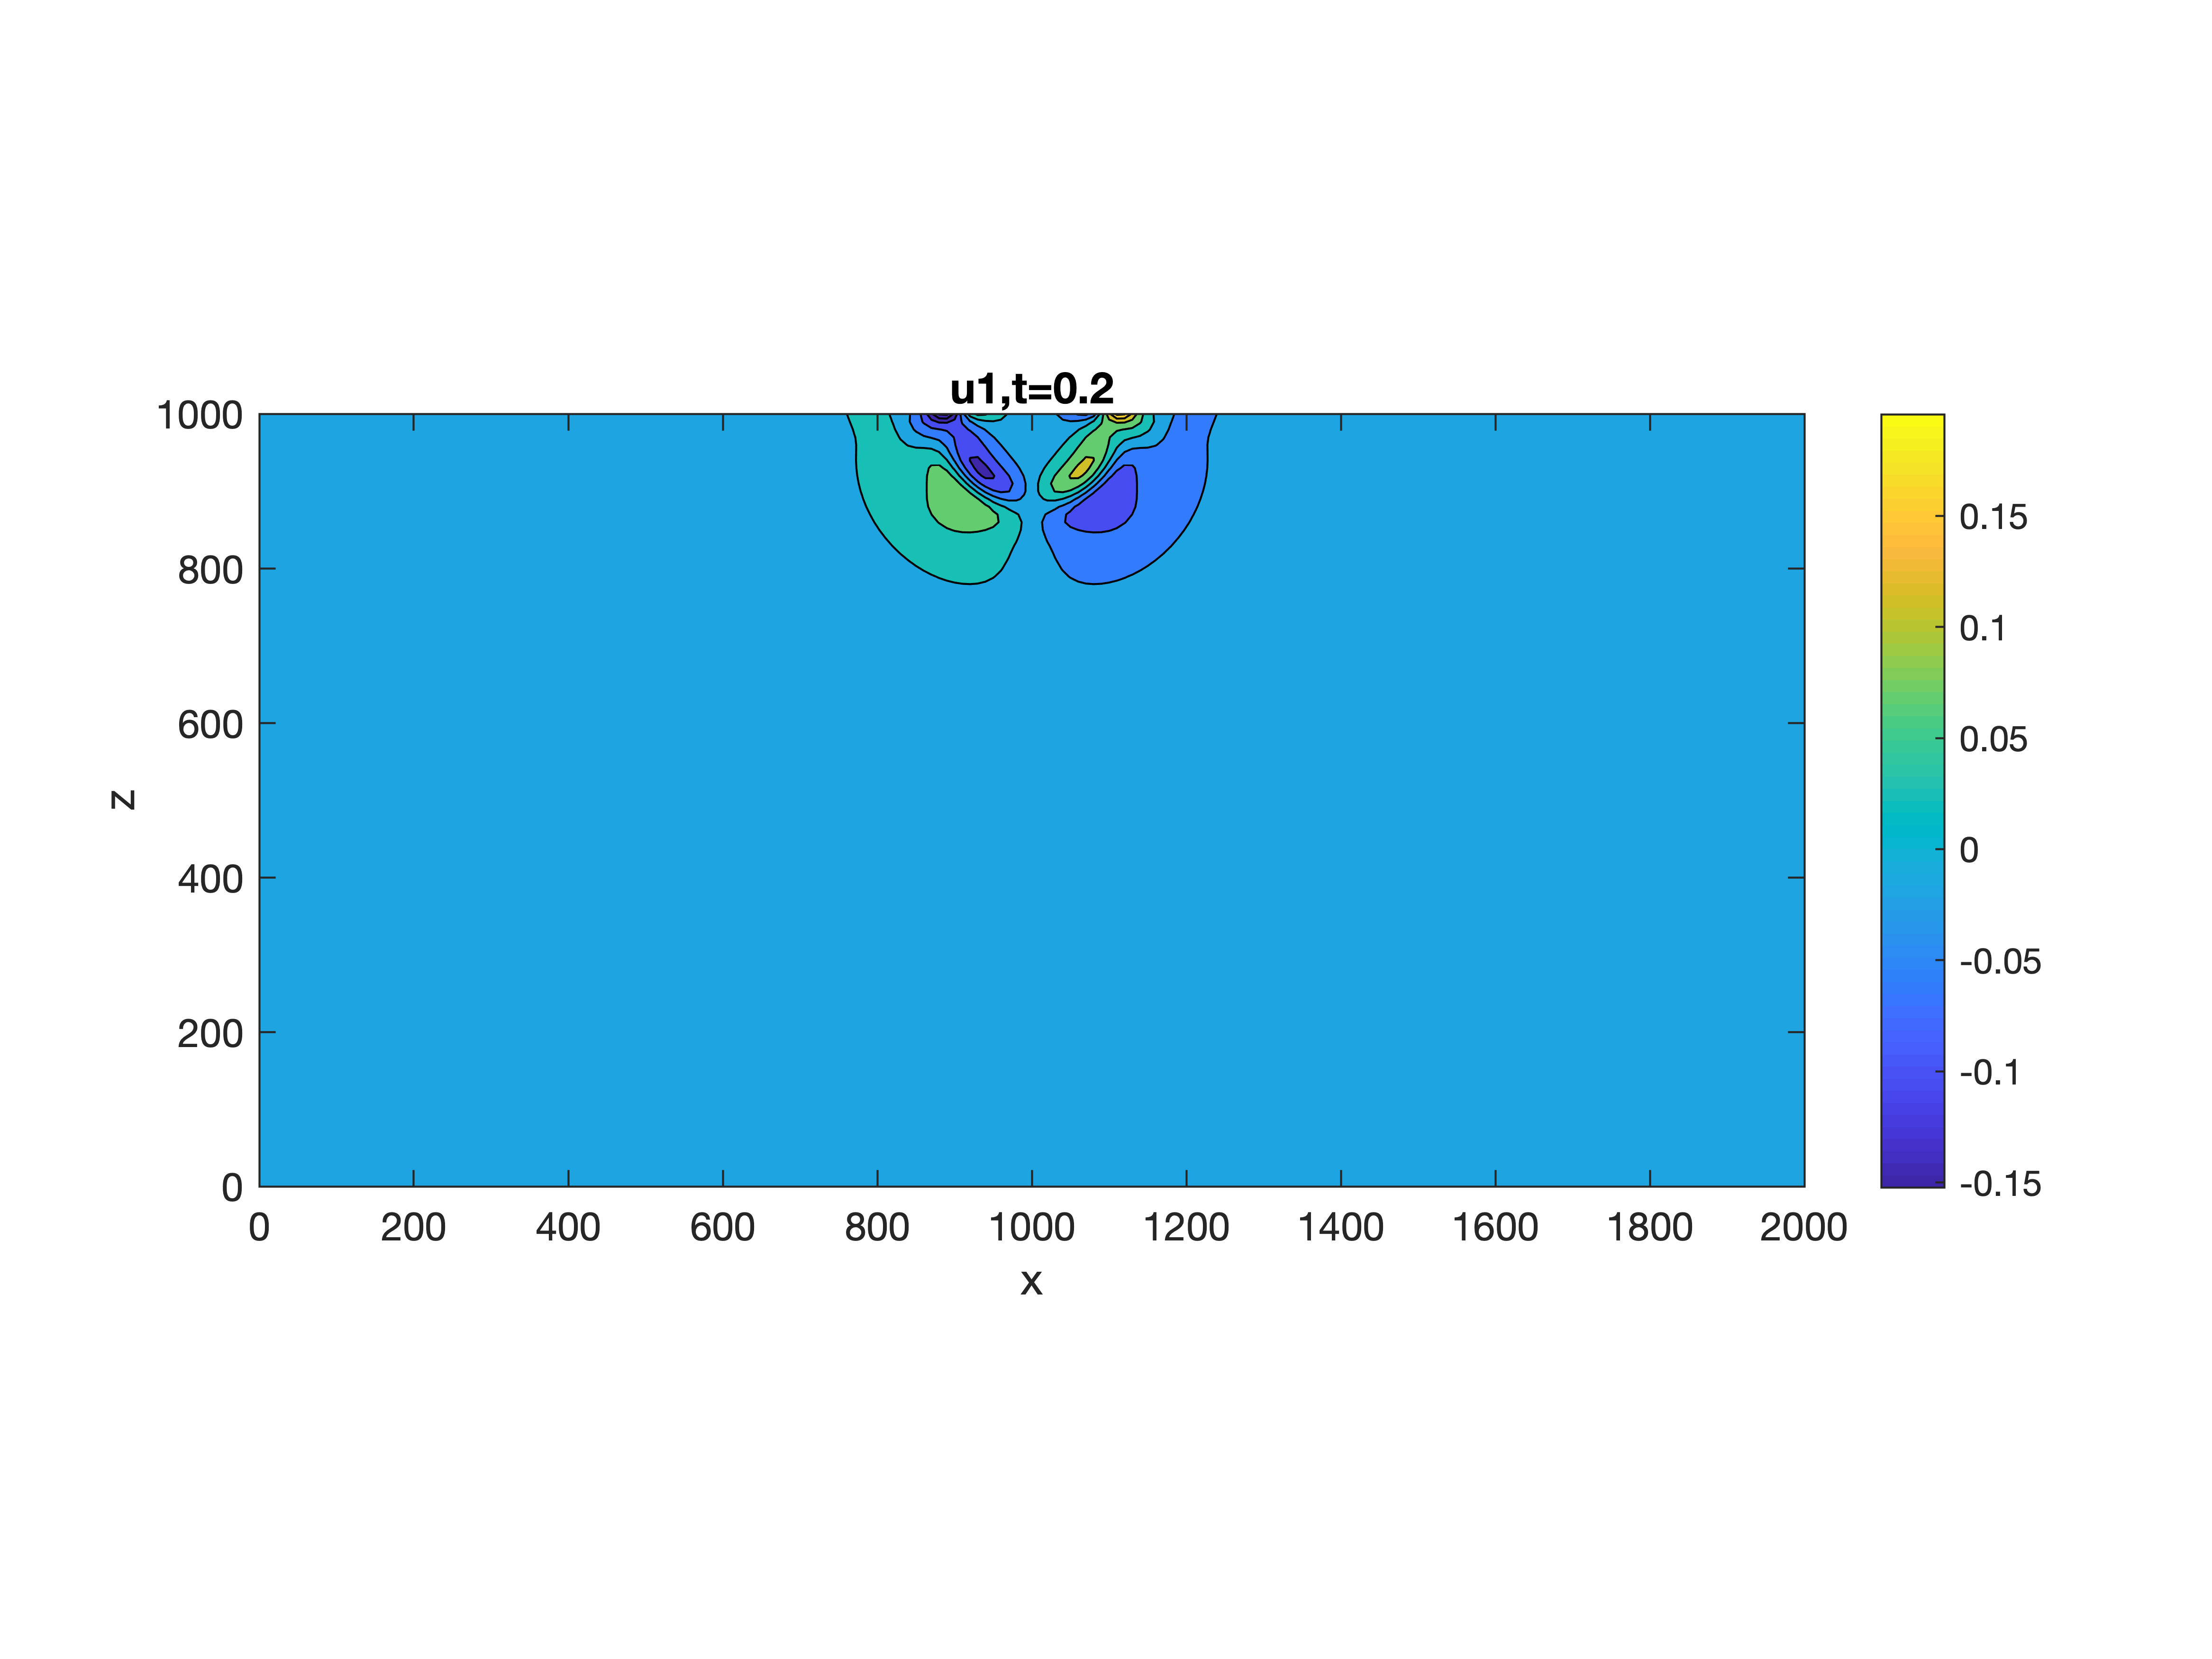
\includegraphics[width=0.45\textwidth]{u1_t02_cartesian.png}
	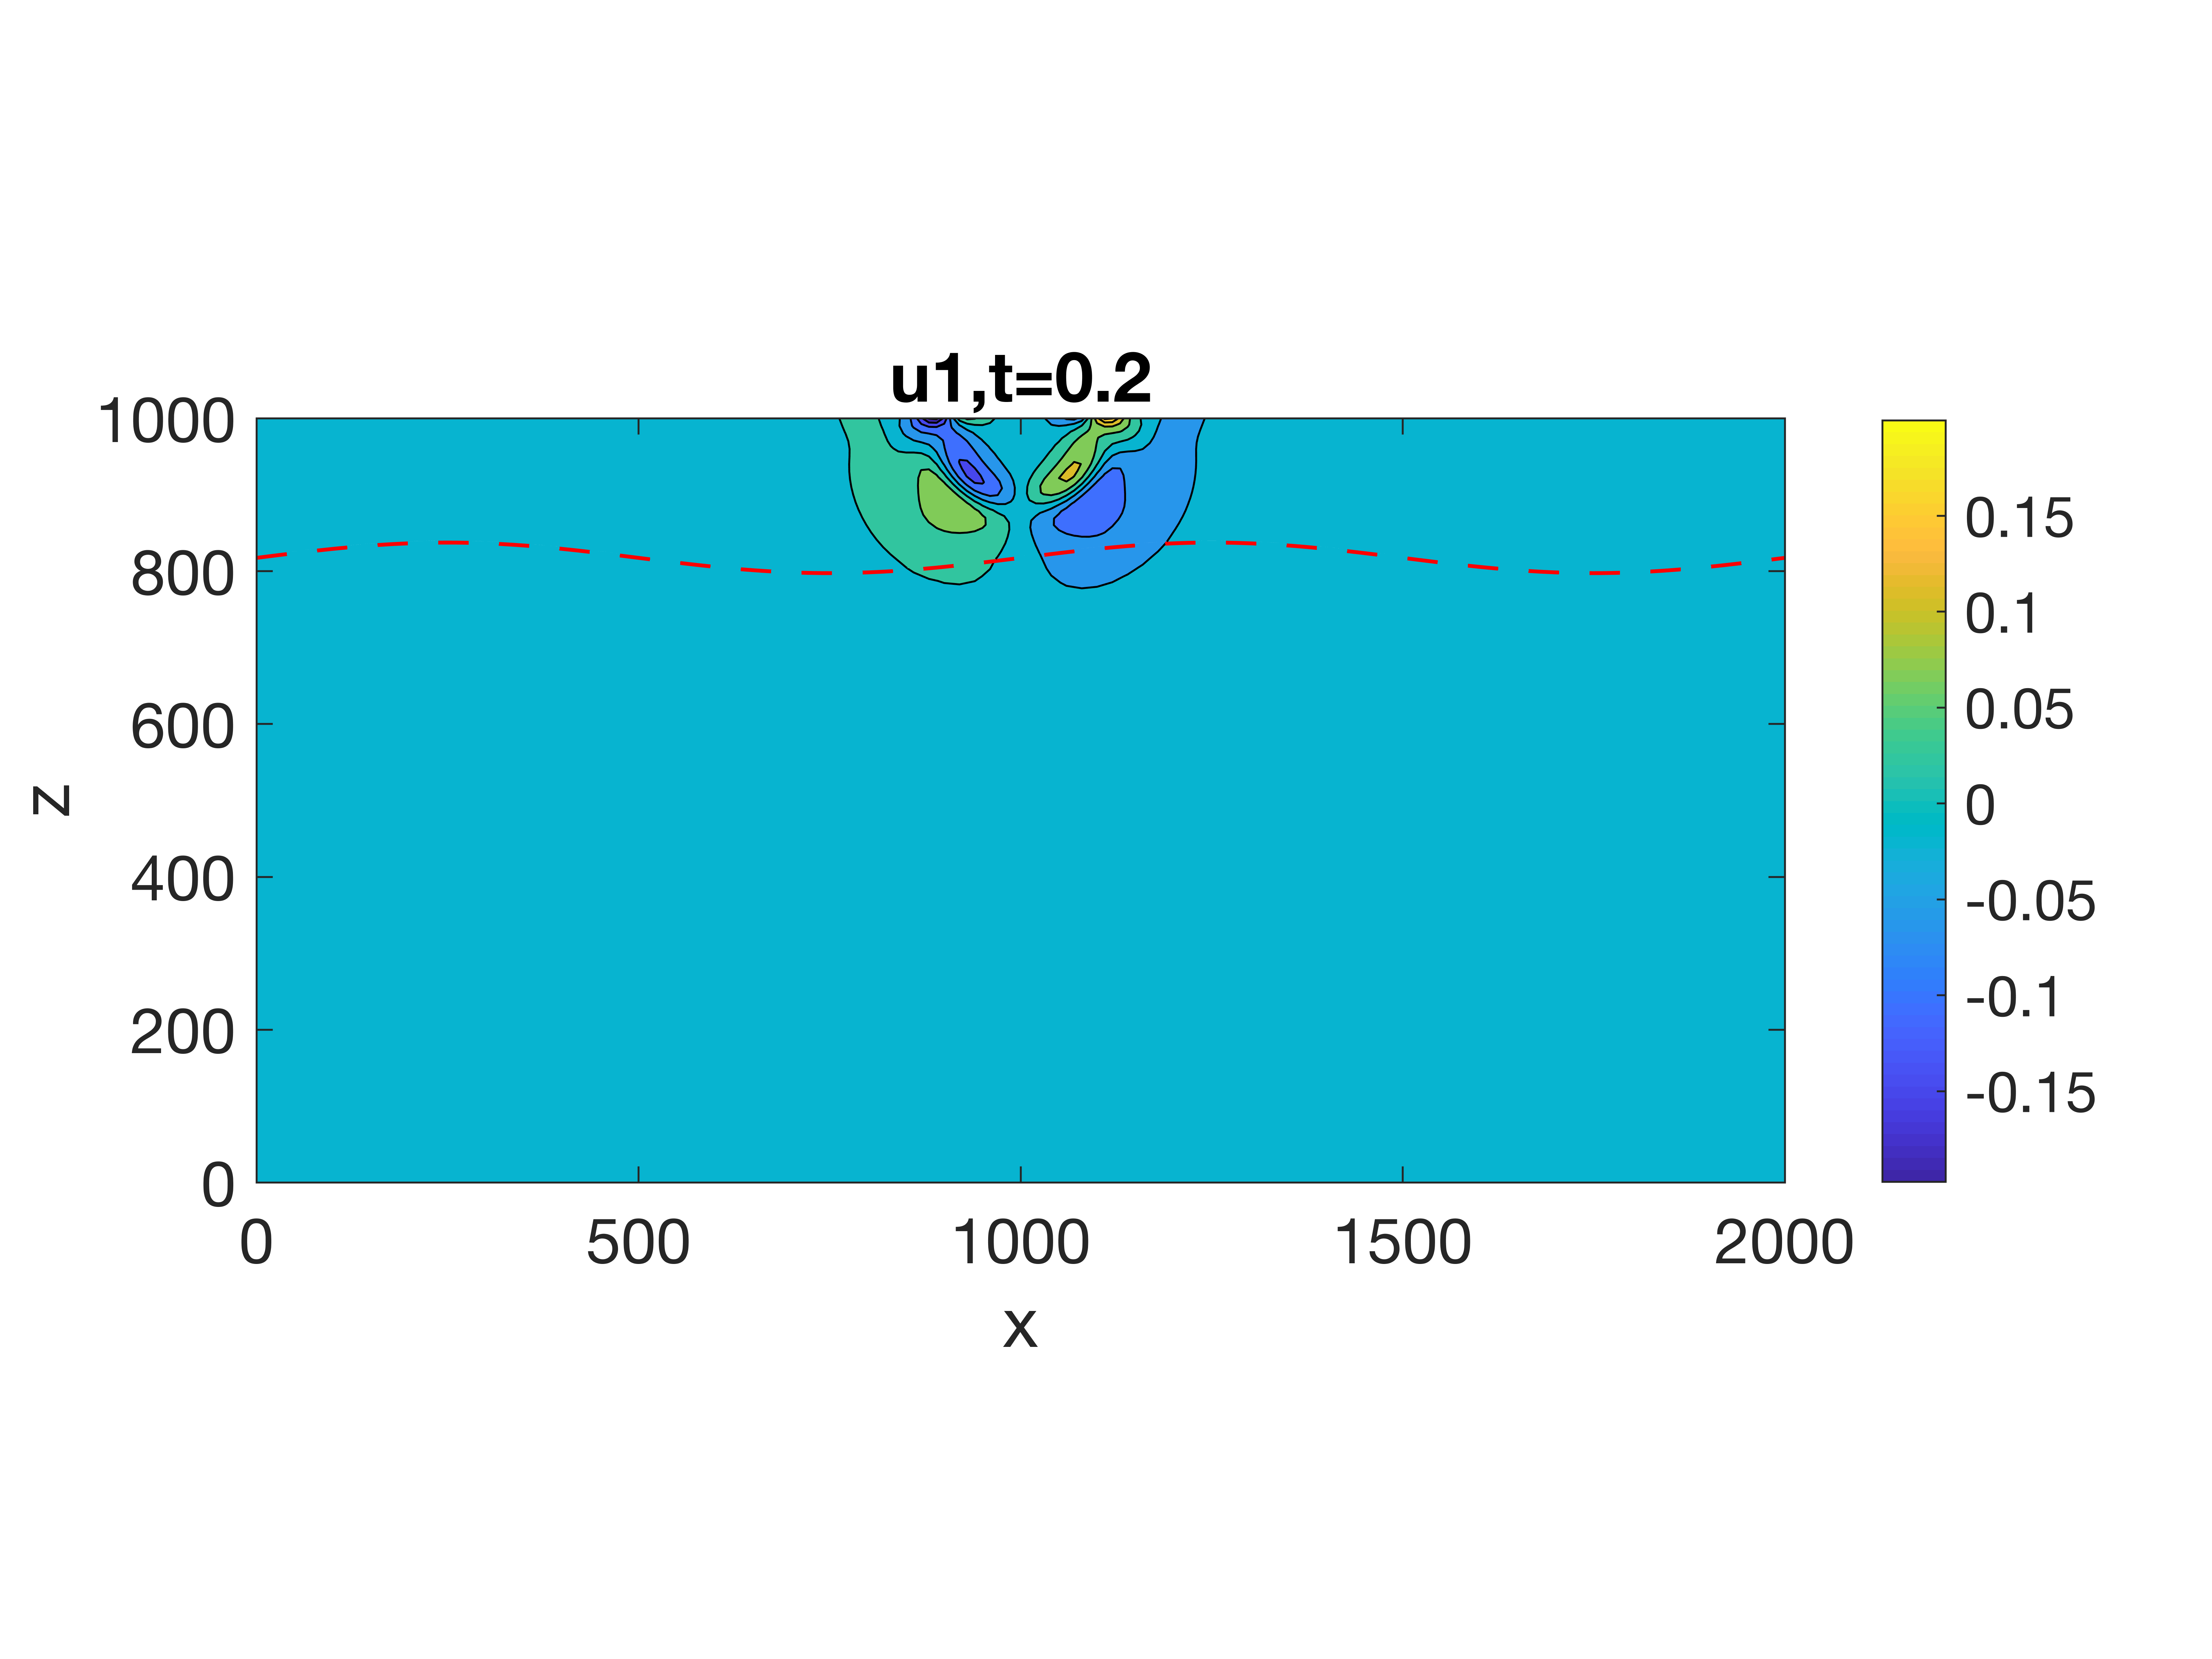
\includegraphics[width=0.45\textwidth]{u1_t02_curvi_mr.png}\\
	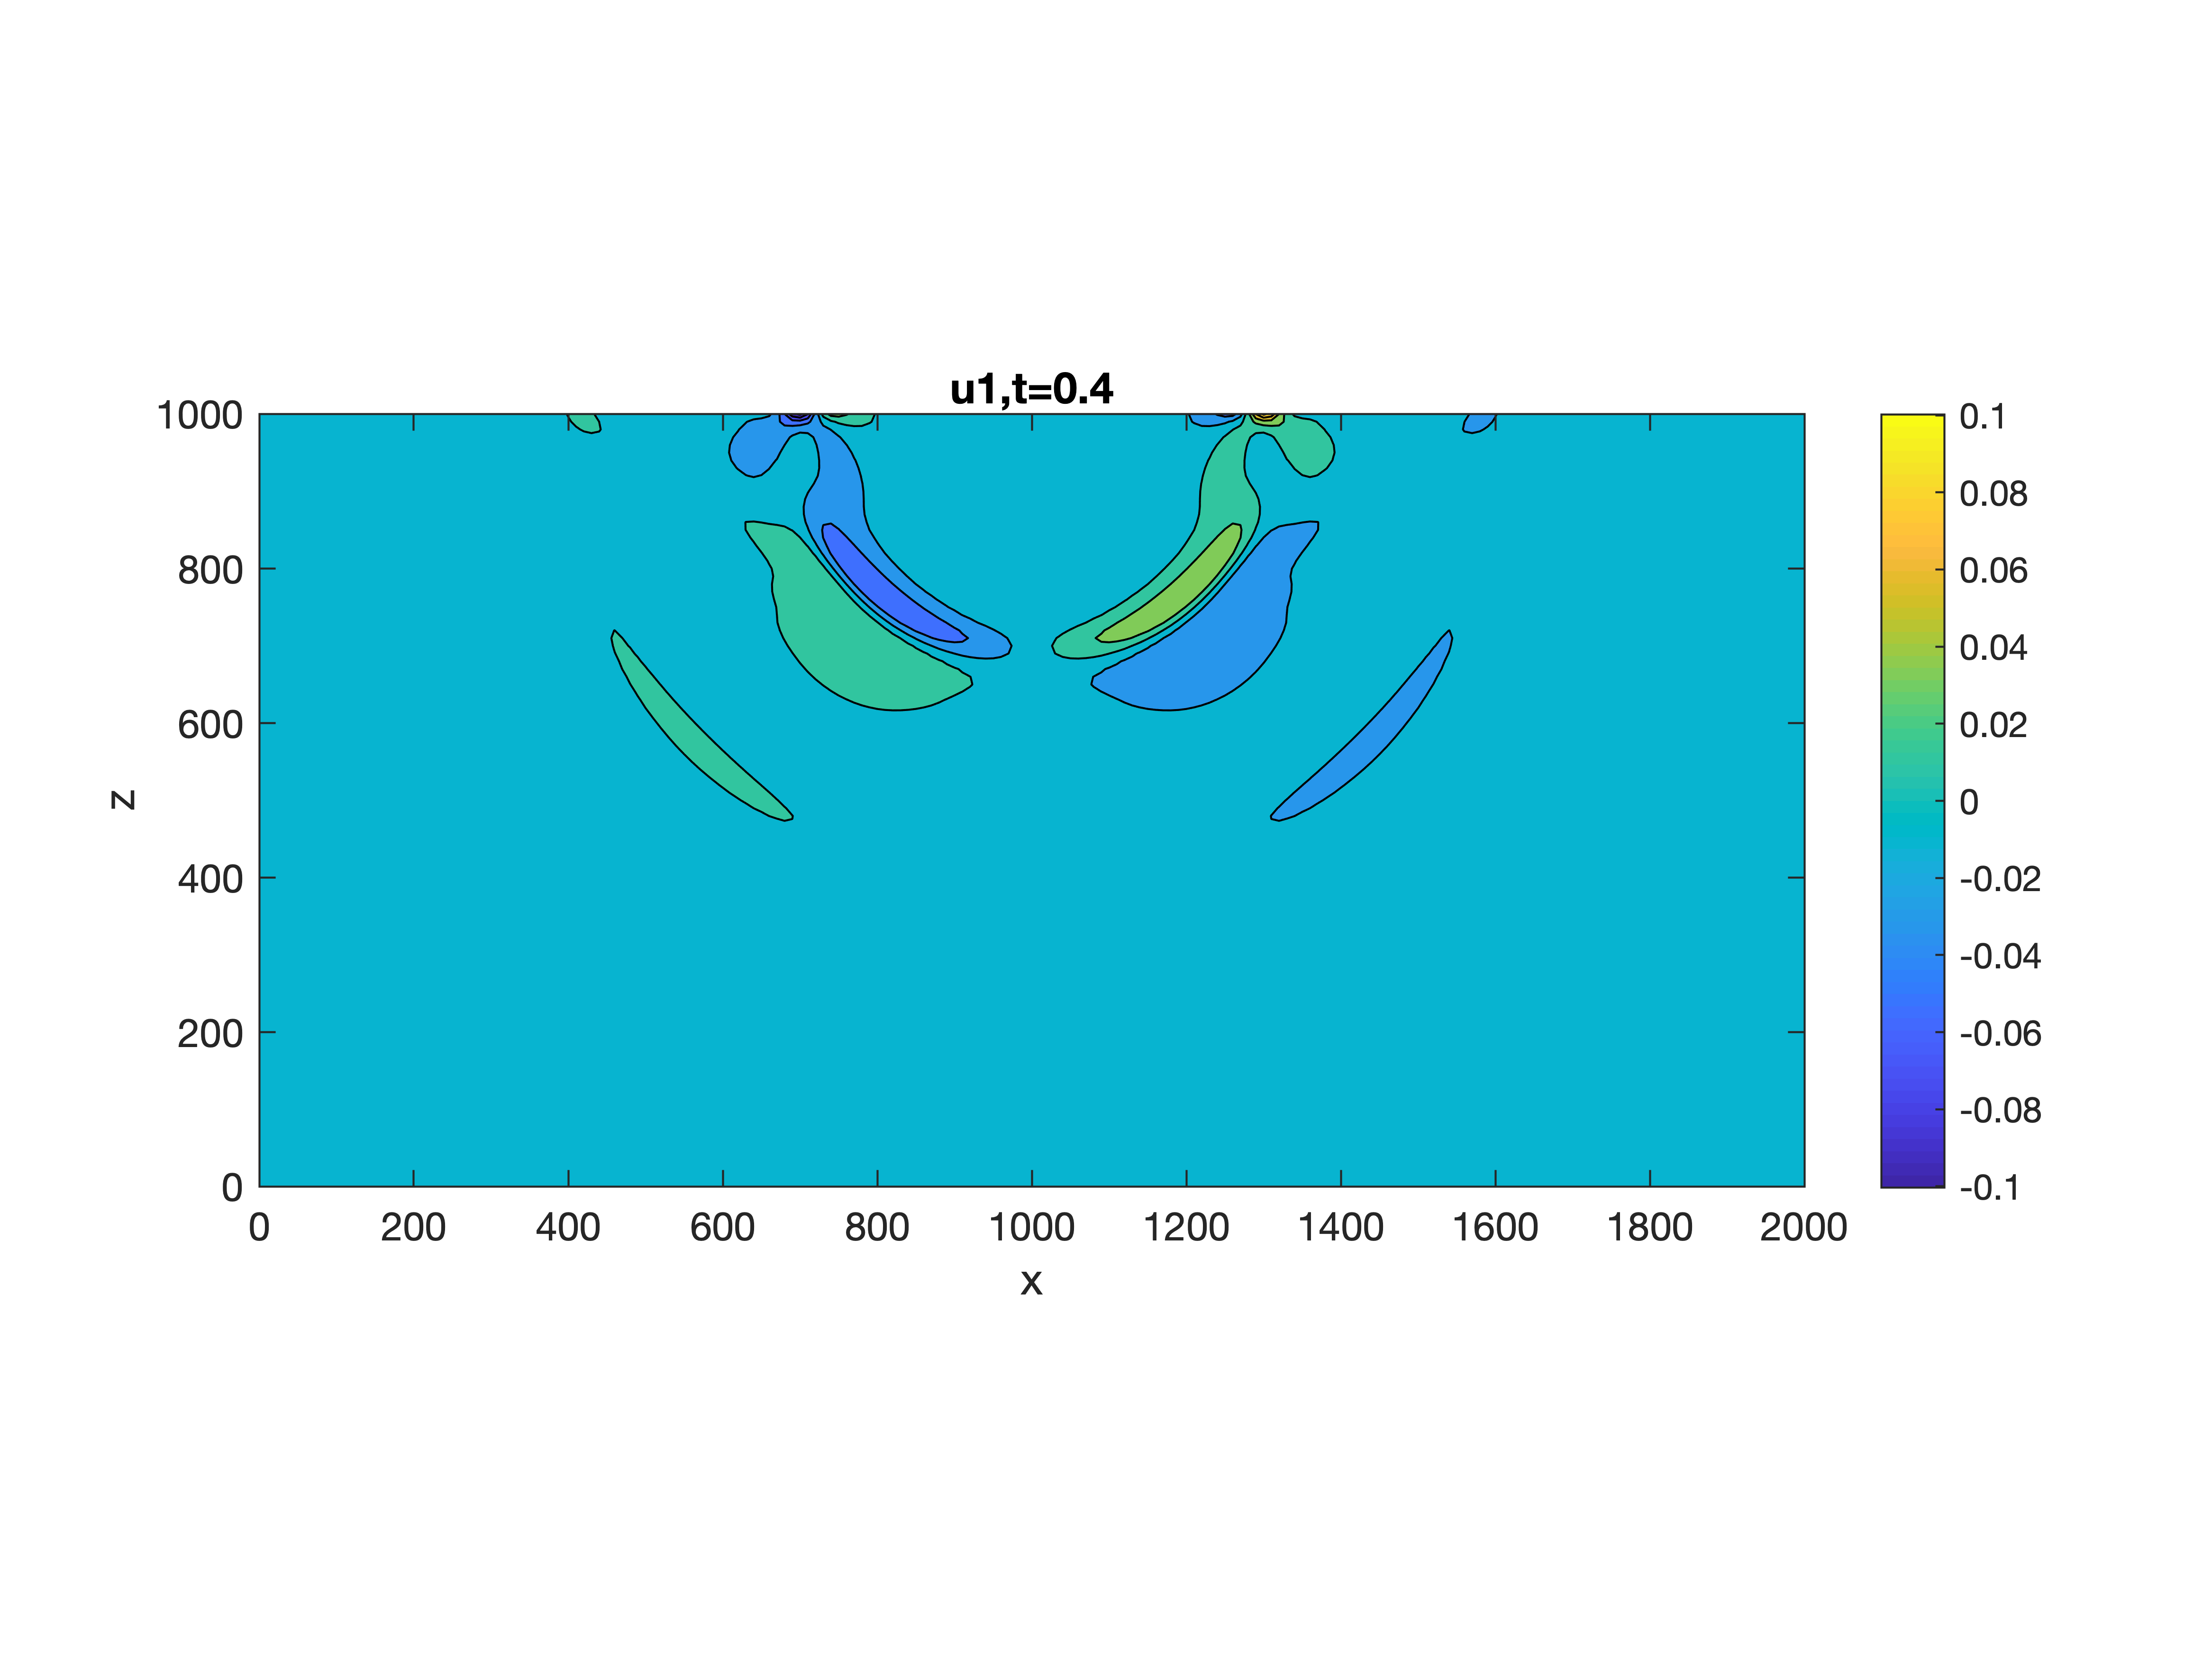
\includegraphics[width=0.45\textwidth]{u1_t04_cartesian.png}
	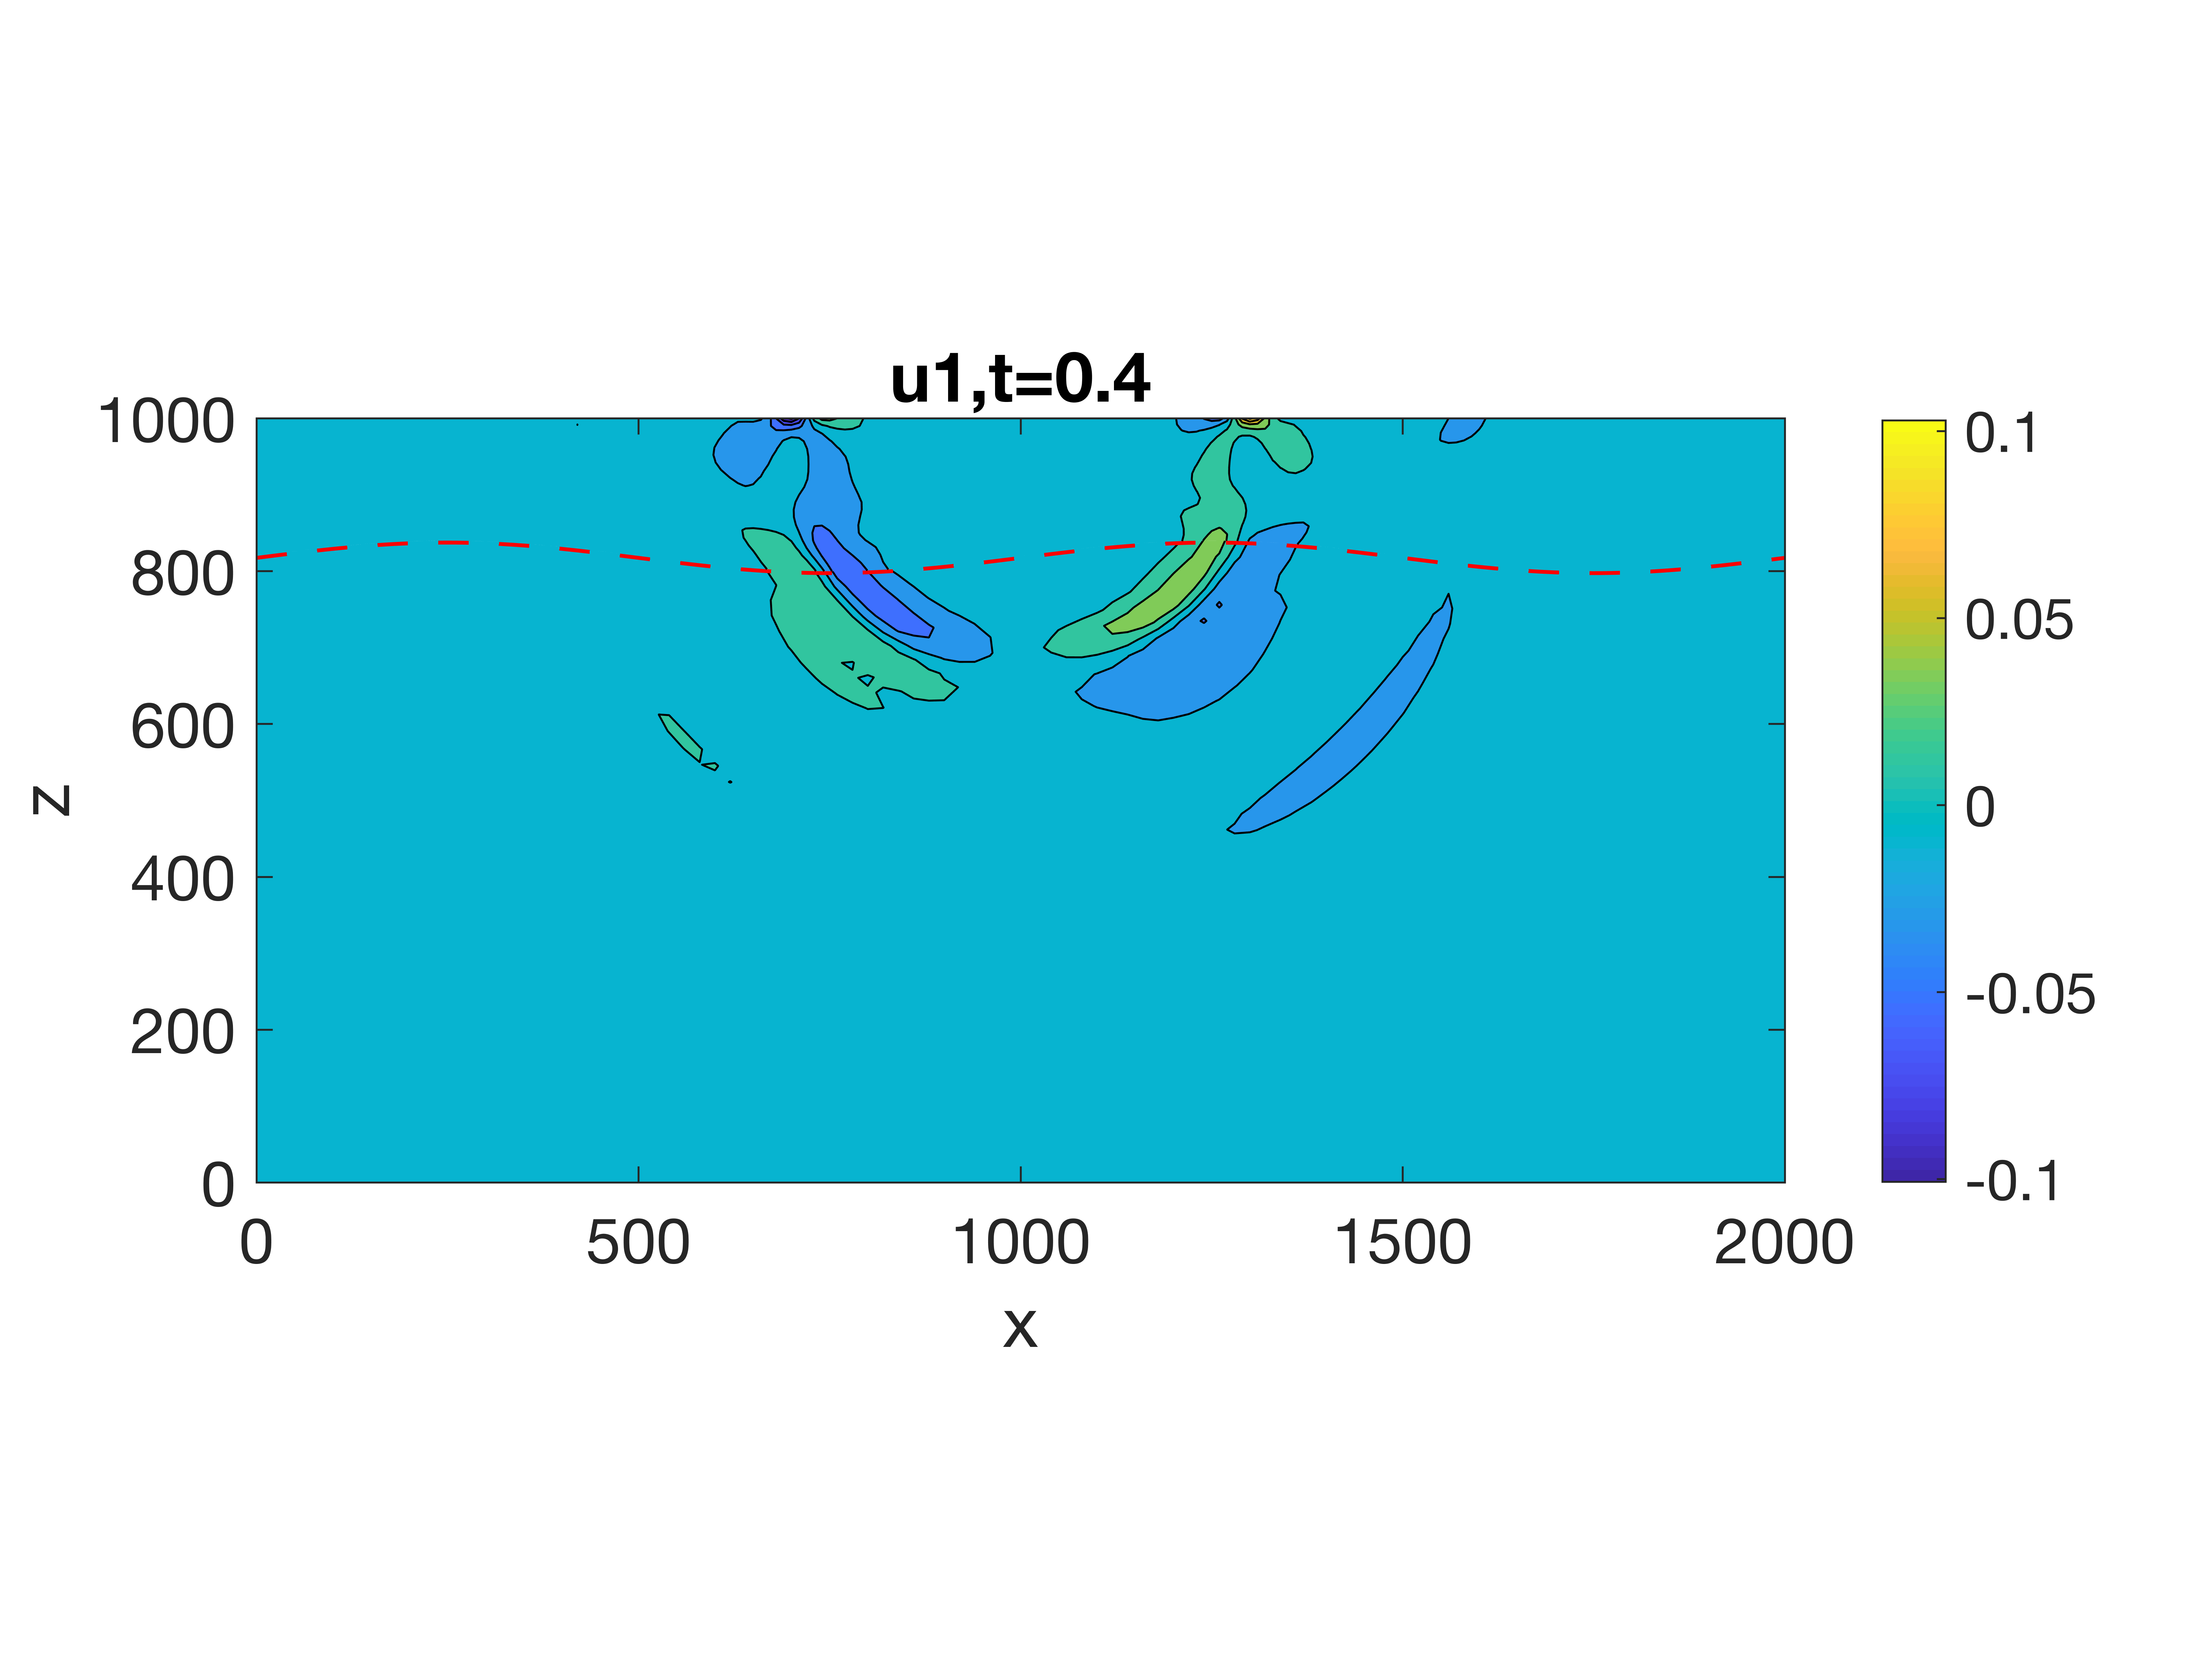
\includegraphics[width=0.45\textwidth]{u1_t04_curvi_mr.png}
	\caption{\scriptsize{The graph for $u_1$. From left to right are for Cartesian mesh without mesh refinement and curvi-linear mesh with mesh refinement respectively. From top to bottom are for $t = 0.2$ and $t = 0.4$ respectively.}}\label{u1}
\end{figure}

\begin{figure}[H]
	\centering
	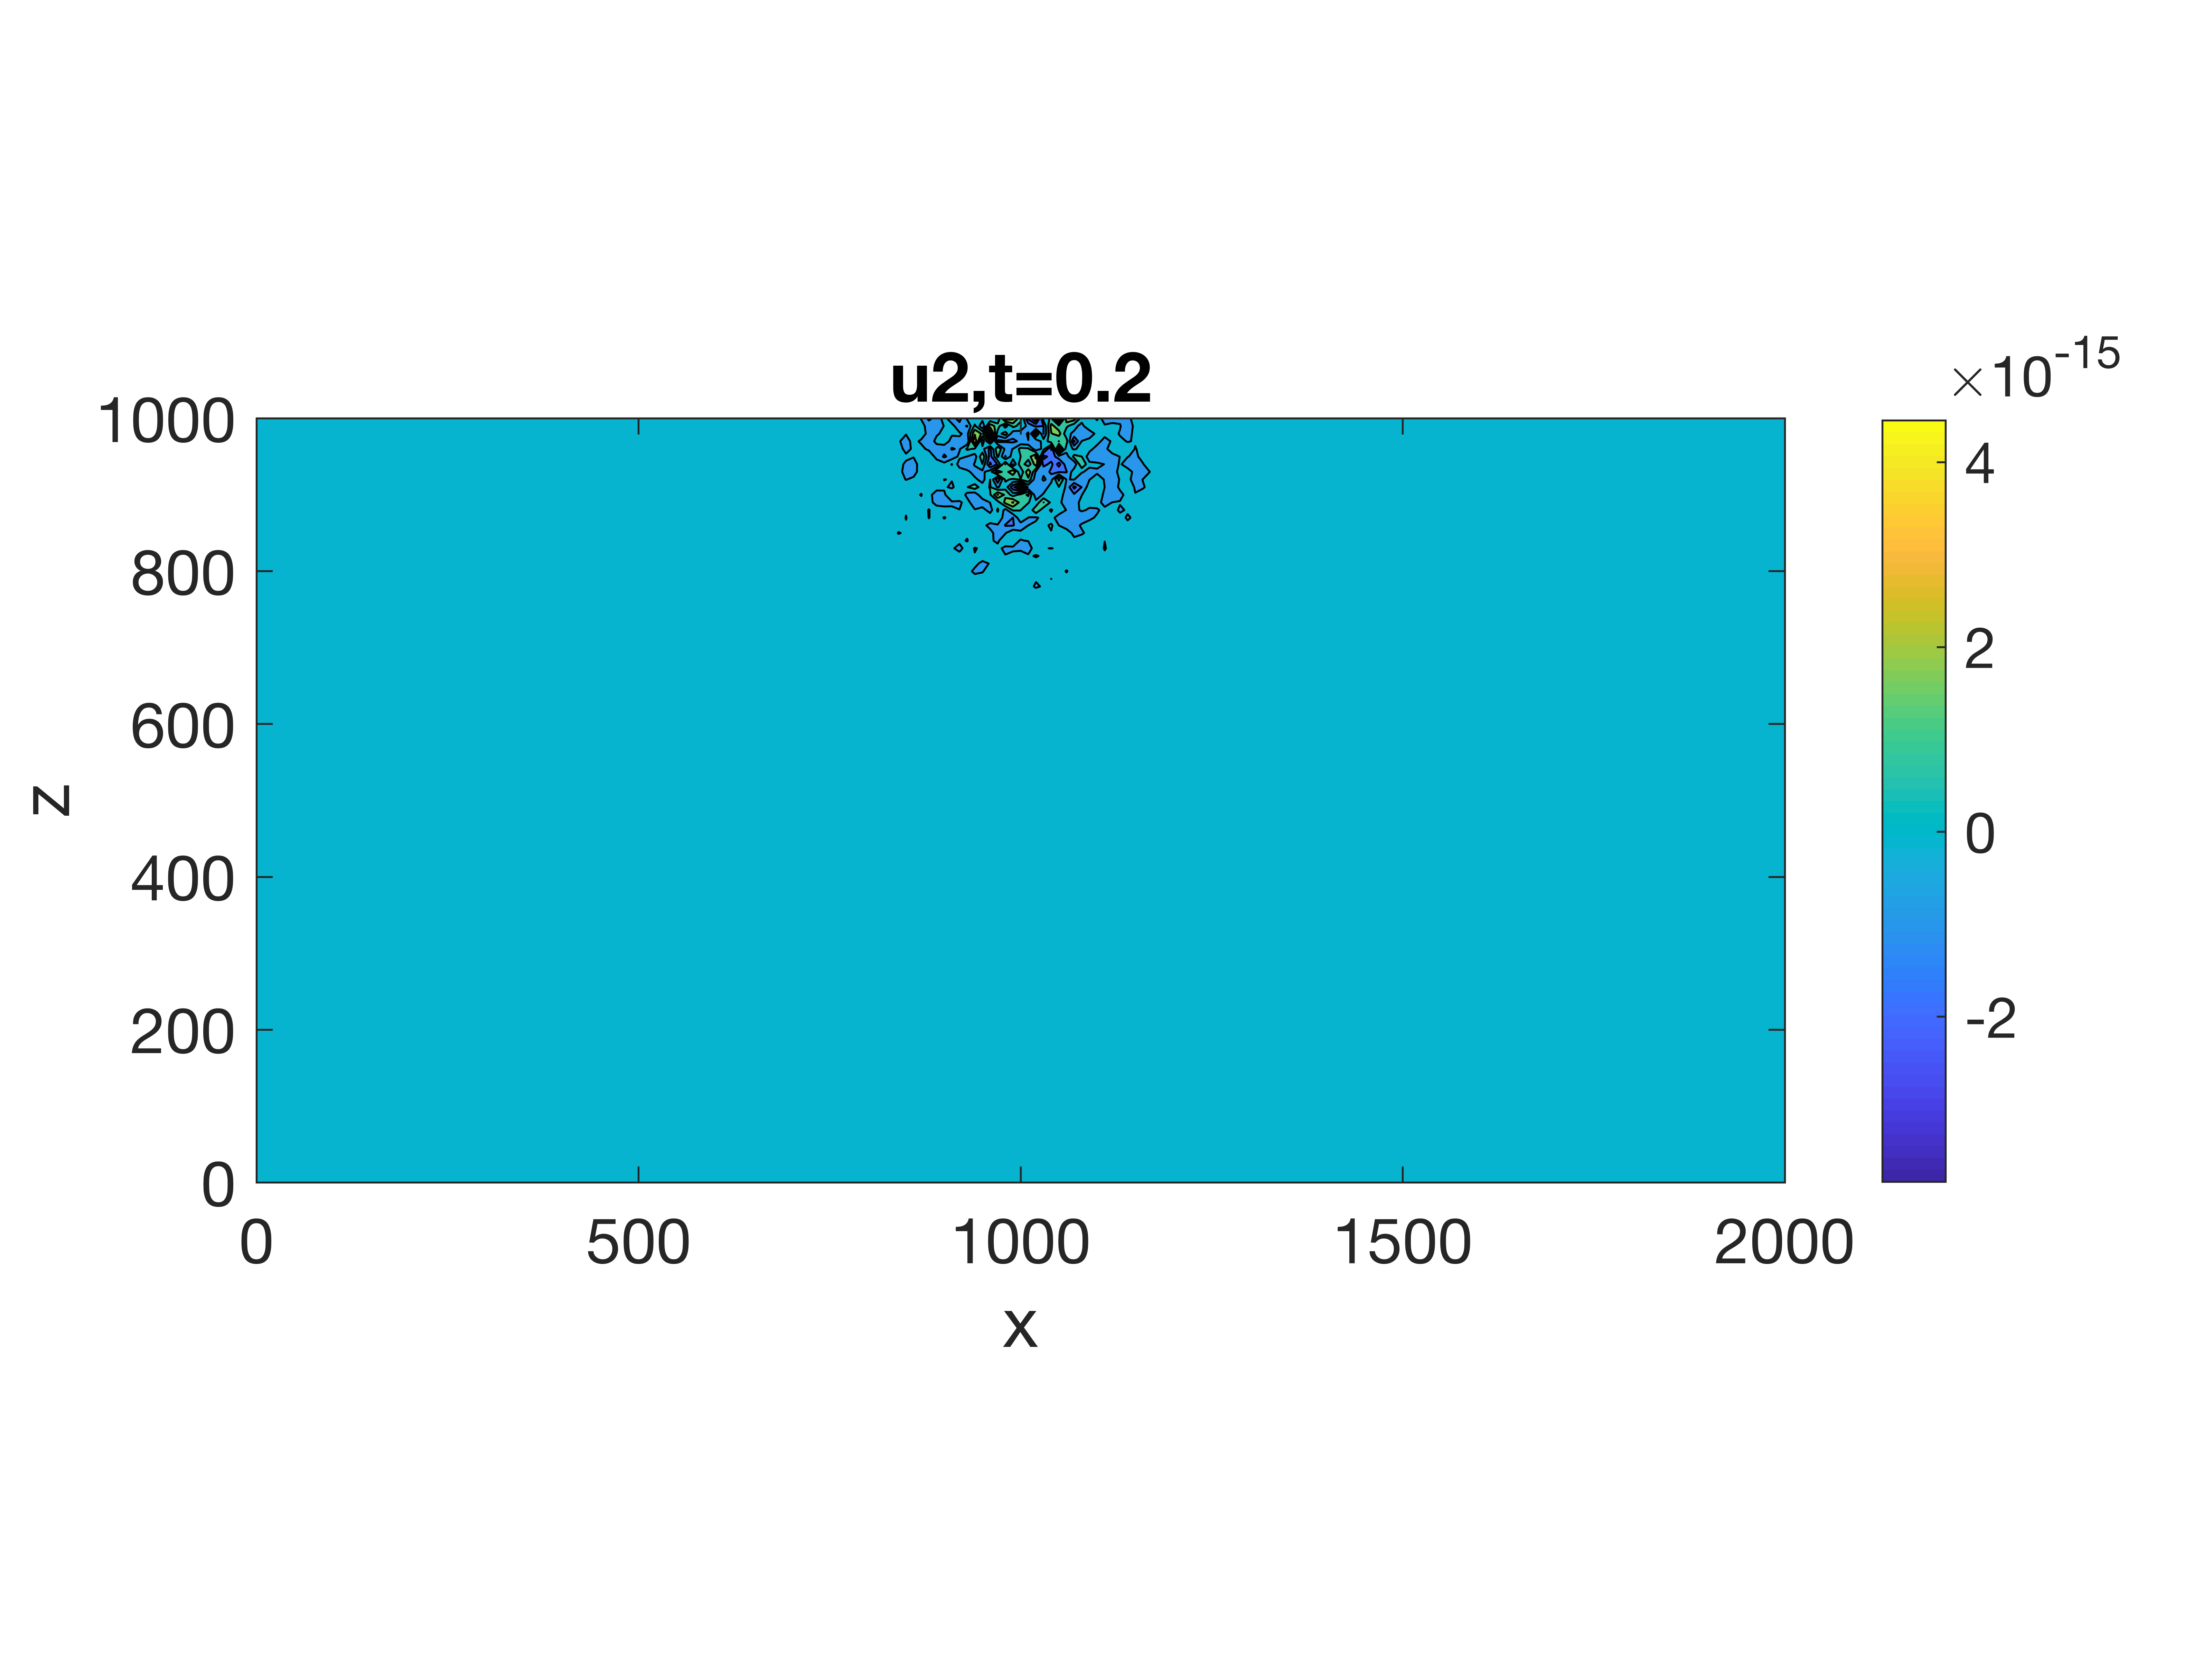
\includegraphics[width=0.45\textwidth]{u2_t02_cartesian.png}
	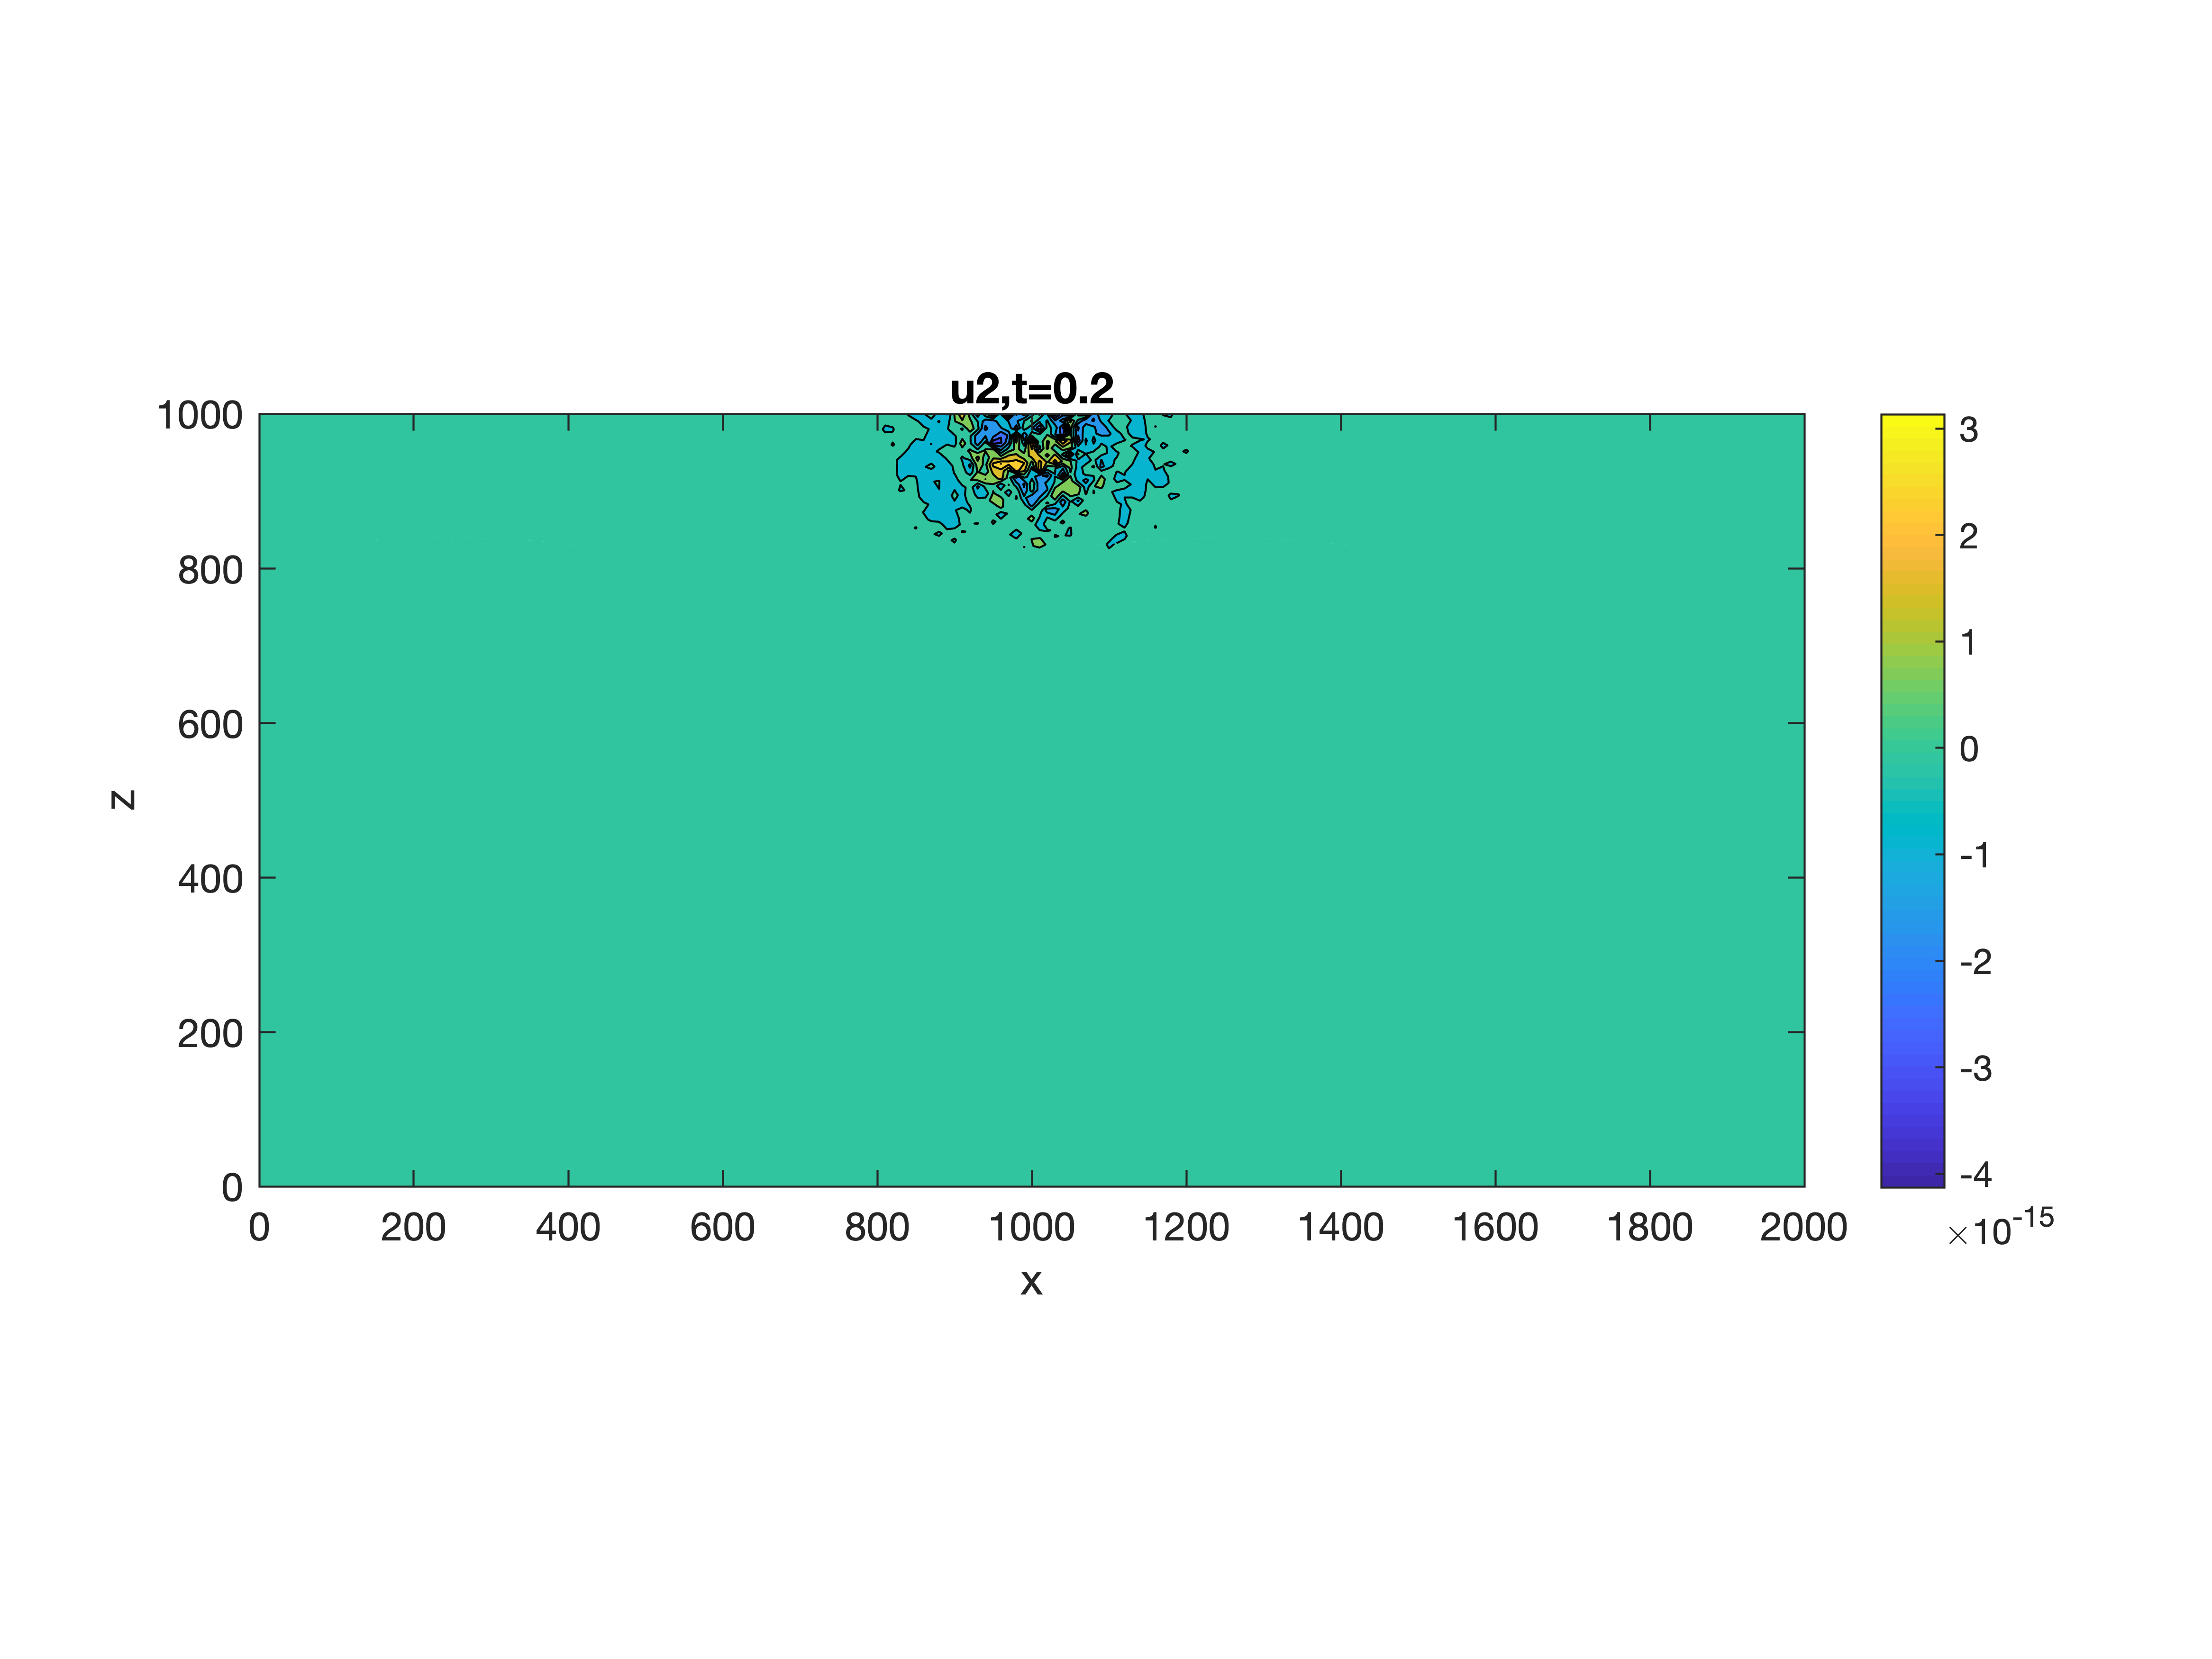
\includegraphics[width=0.45\textwidth]{u2_t02_curvi_mr.png}\\
	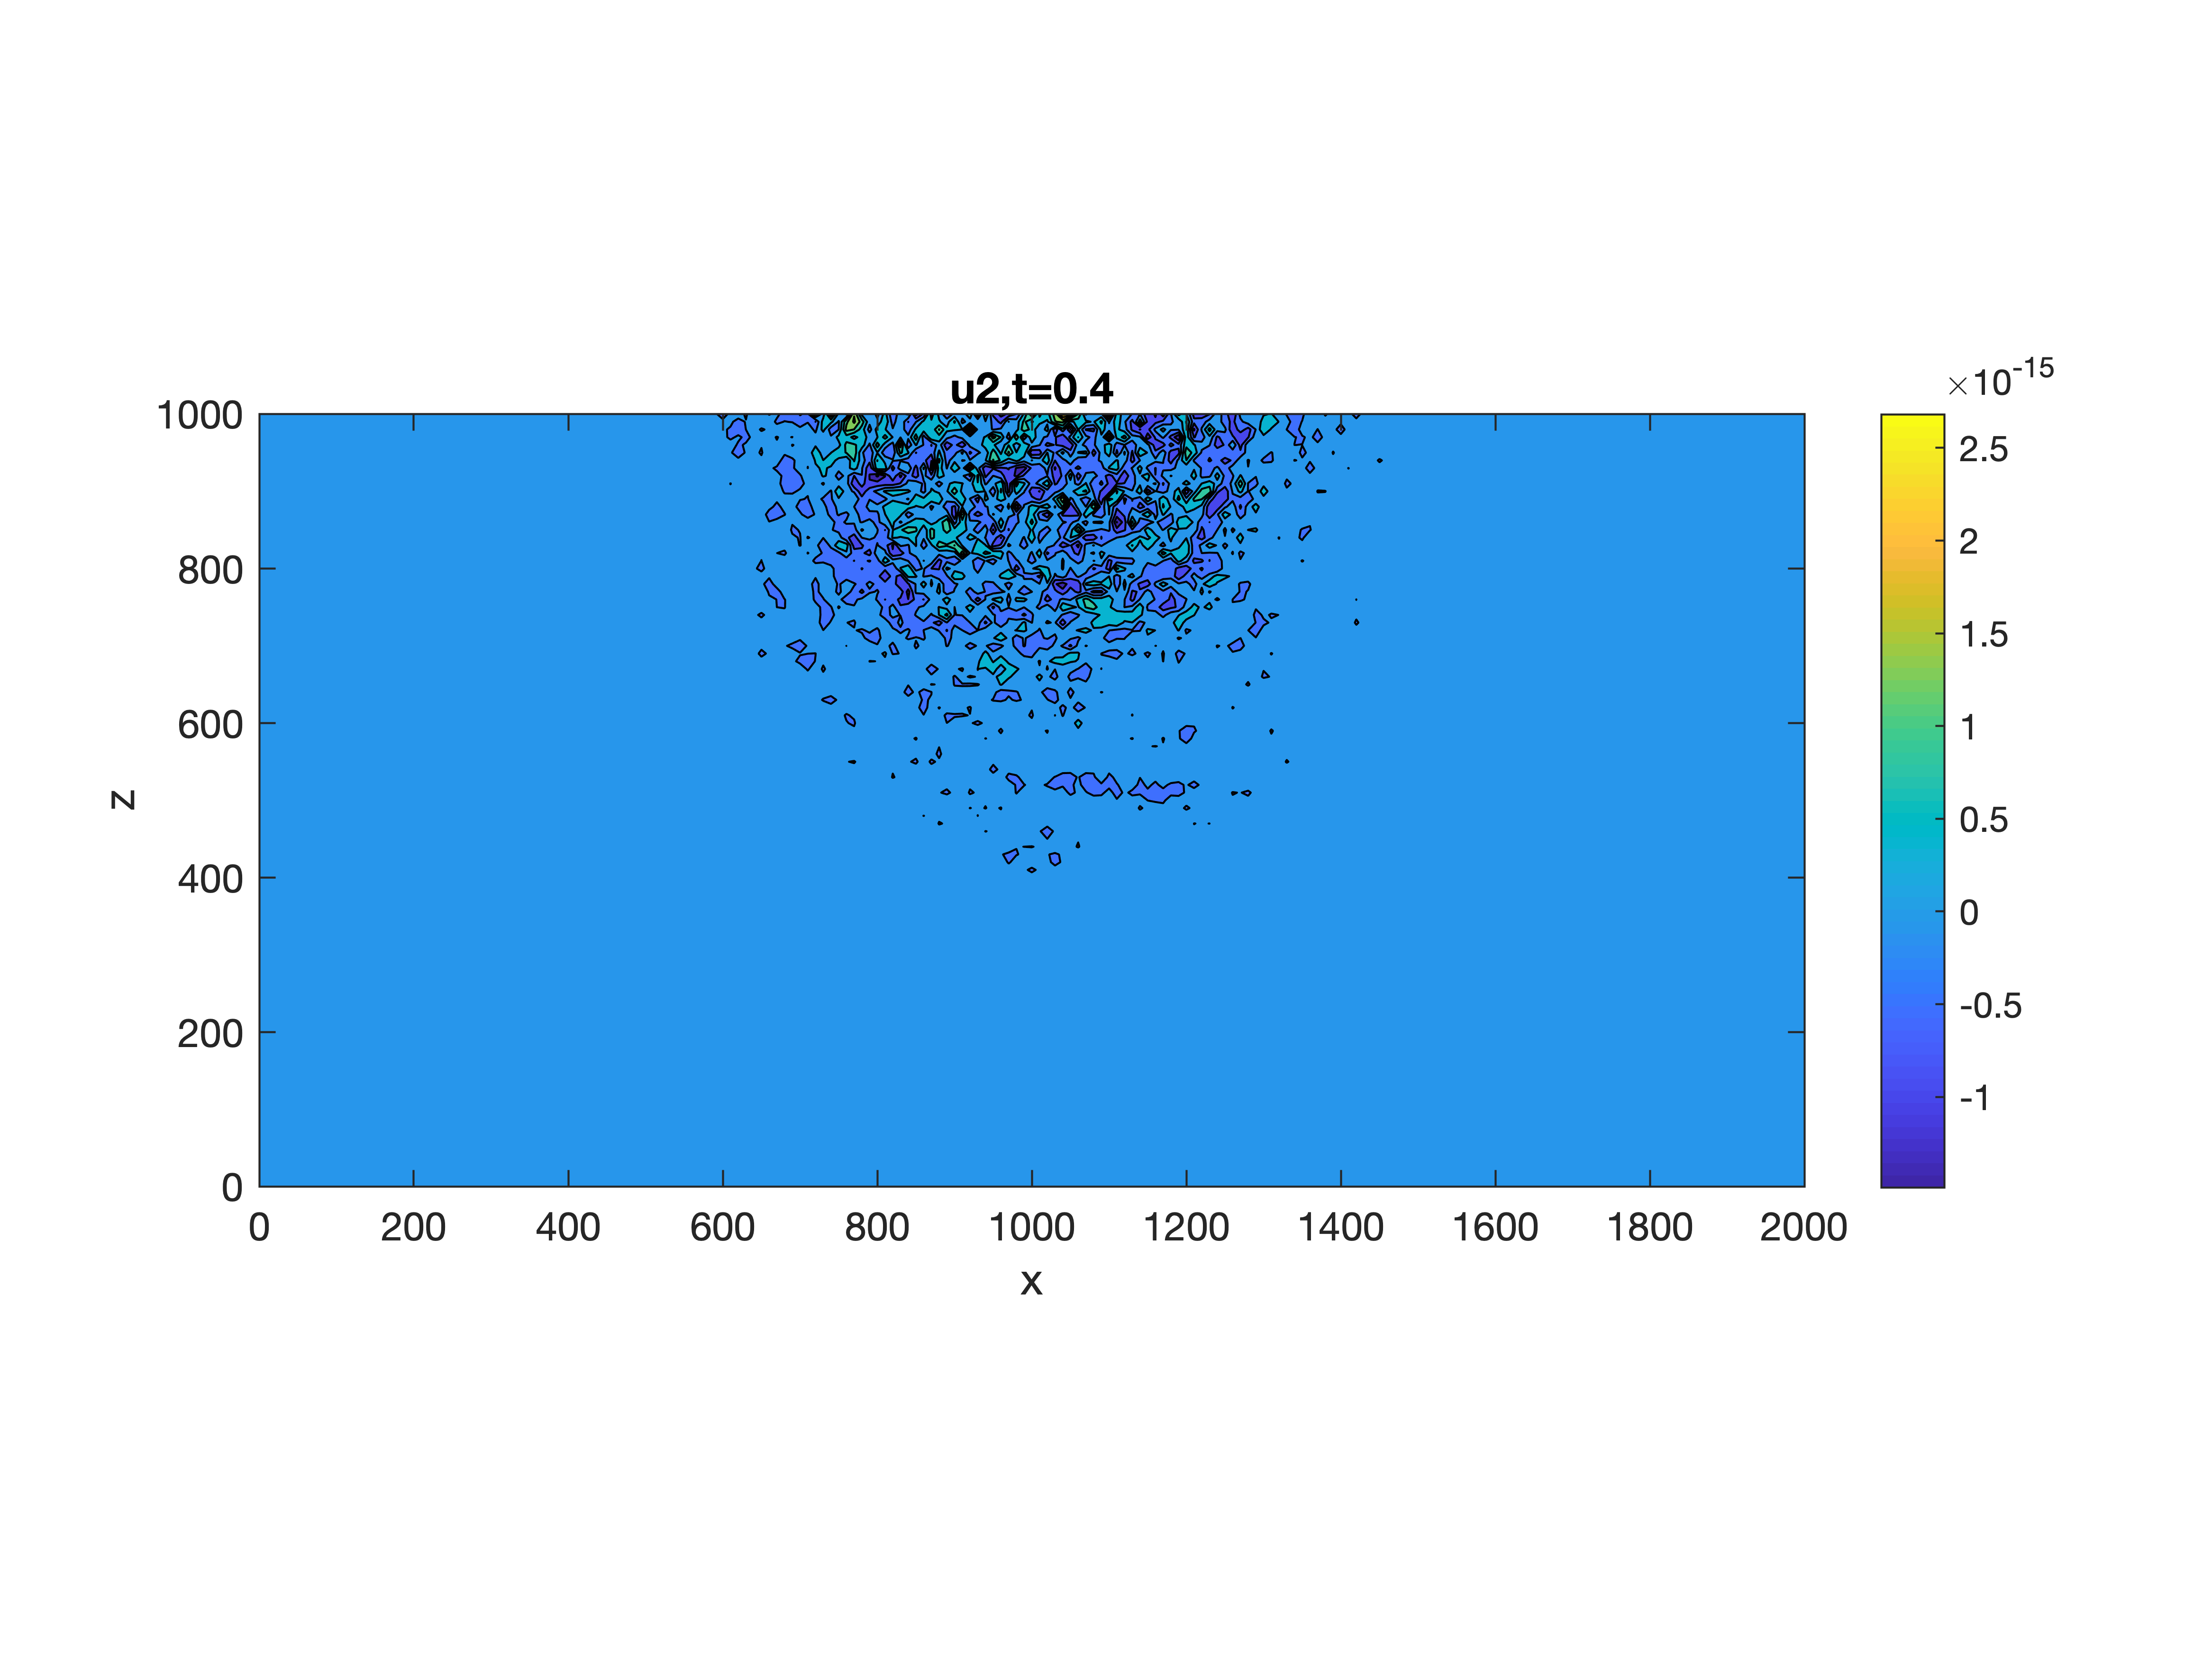
\includegraphics[width=0.45\textwidth]{u2_t04_cartesian.png}
	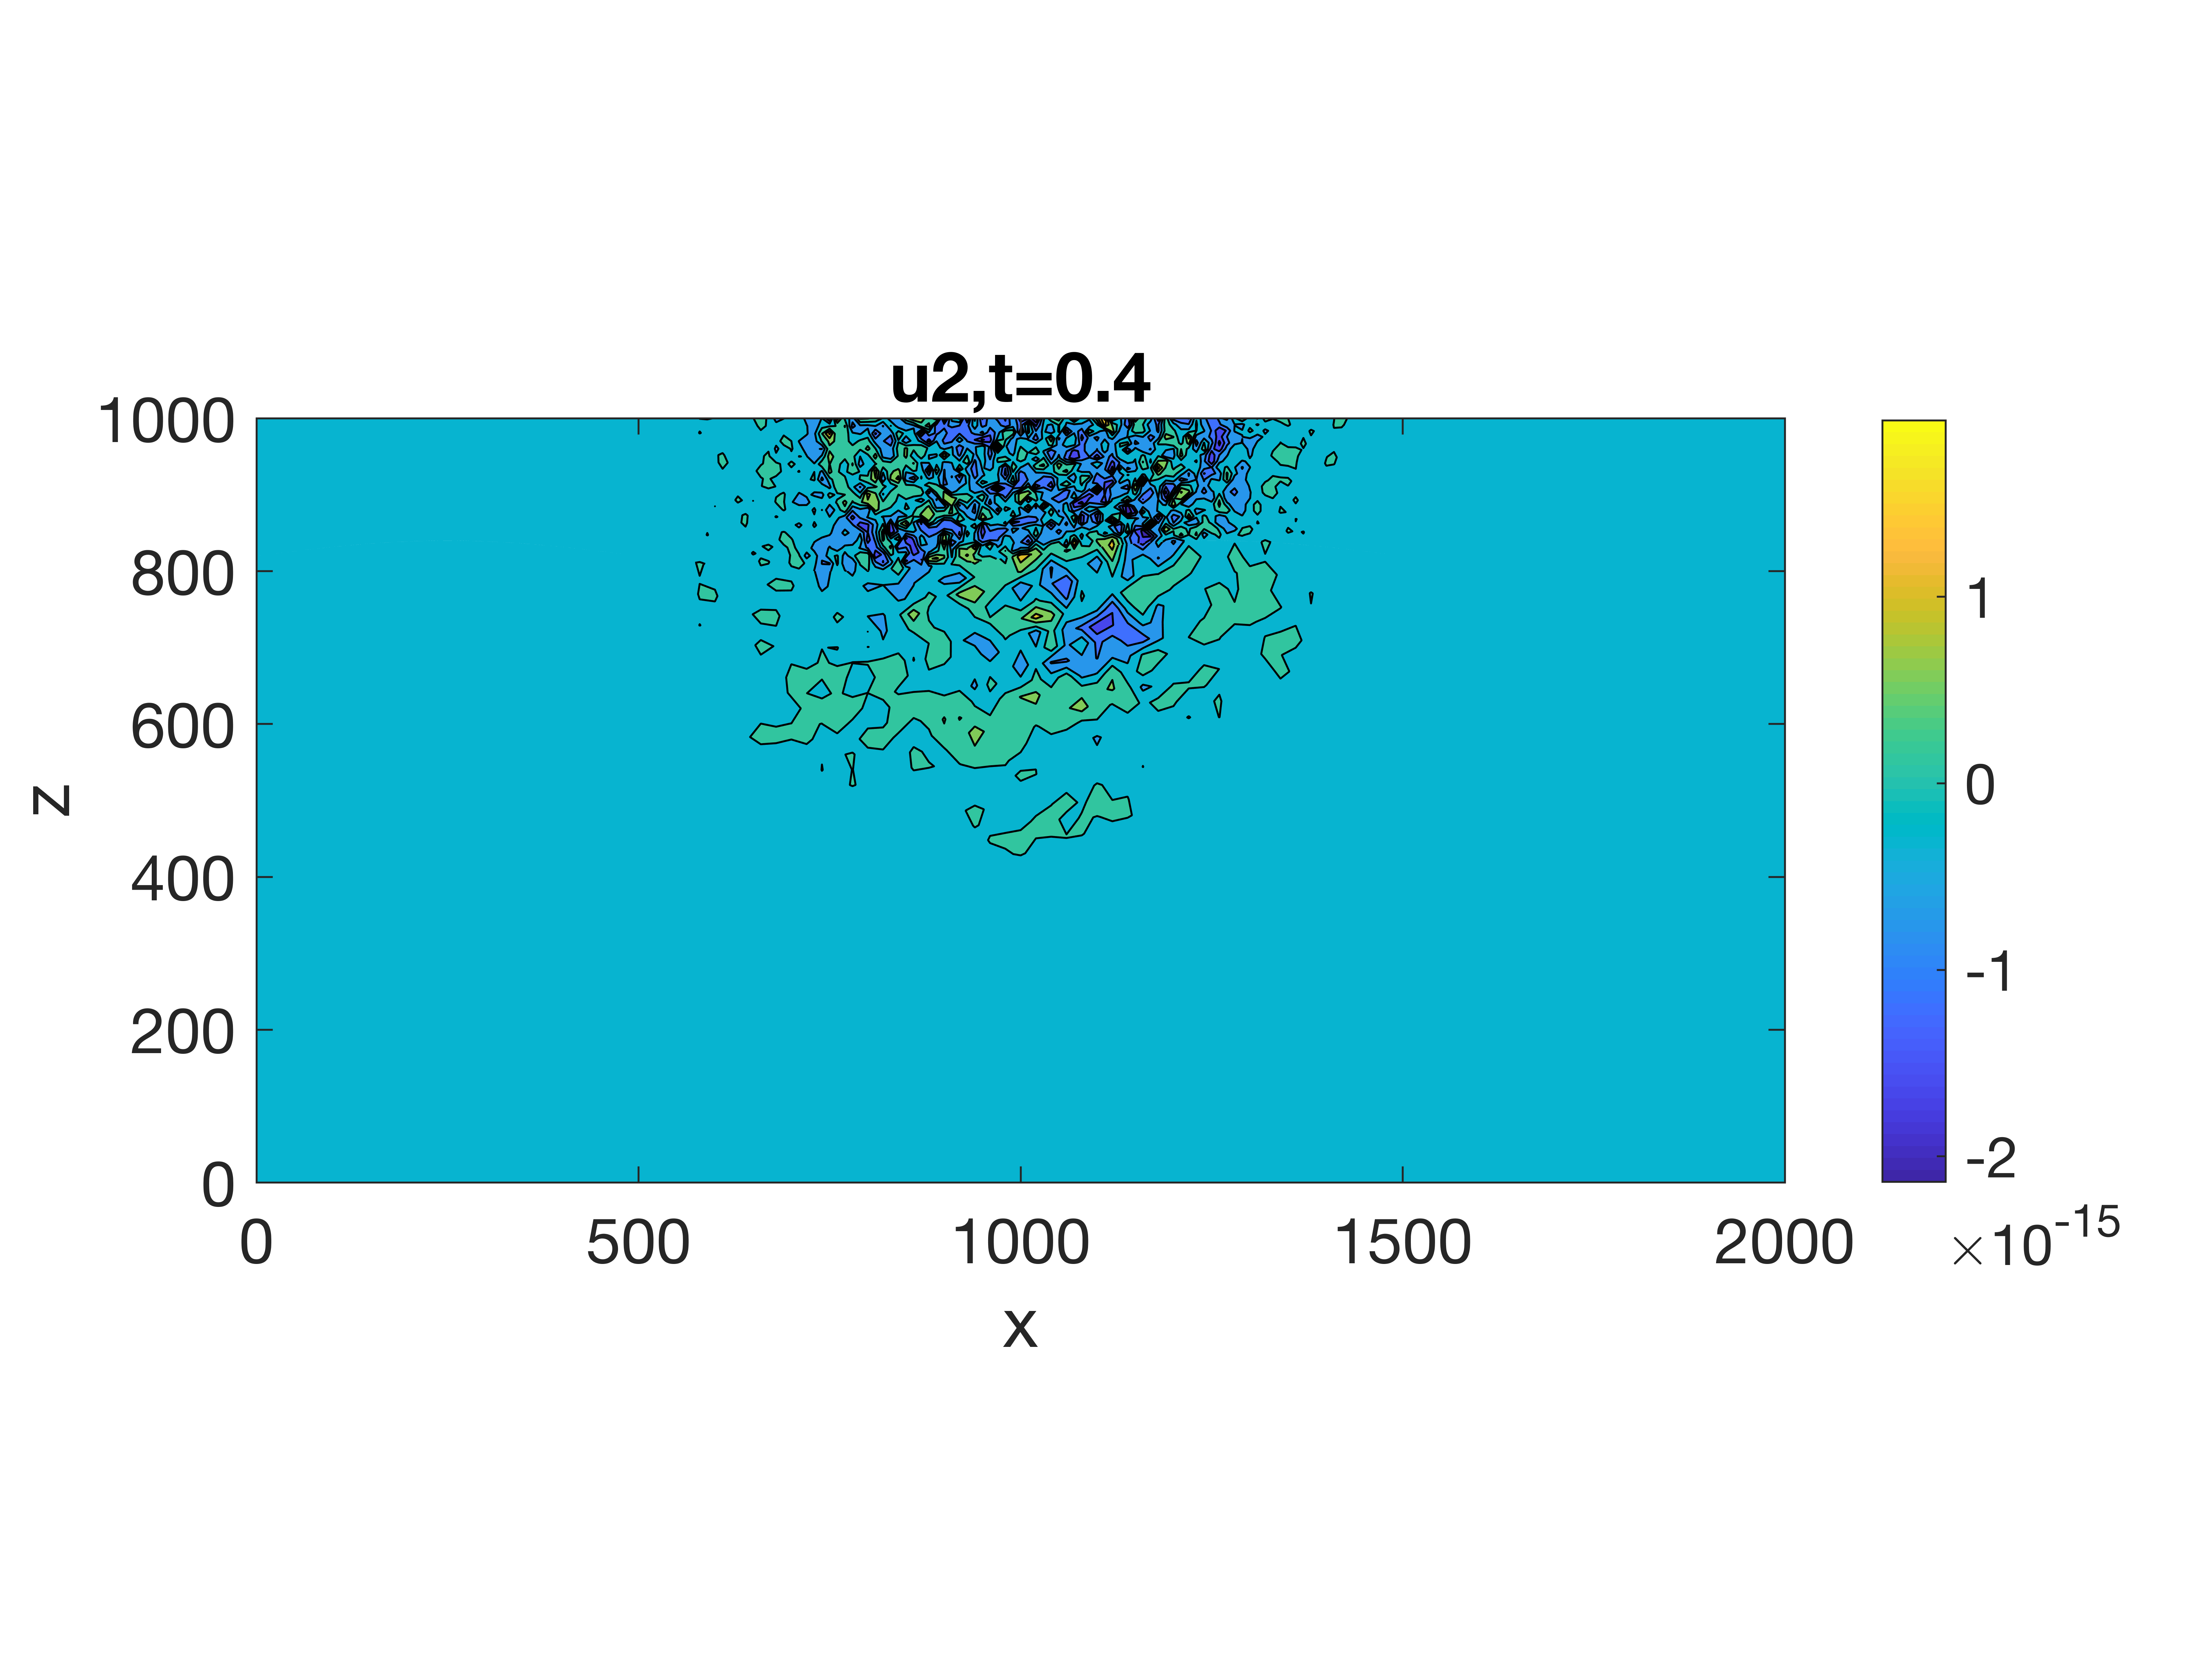
\includegraphics[width=0.45\textwidth]{u2_t04_curvi_mr.png}
	\caption{\scriptsize{The graph for $u_2$. From left to right are for Cartesian mesh without mesh refinement and curvi-linear mesh with mesh refinement respectively. From top to bottom are for $t = 0.2$ and $t = 0.4$ respectively.}}\label{u2}
\end{figure}

\begin{figure}[H]
	\centering
	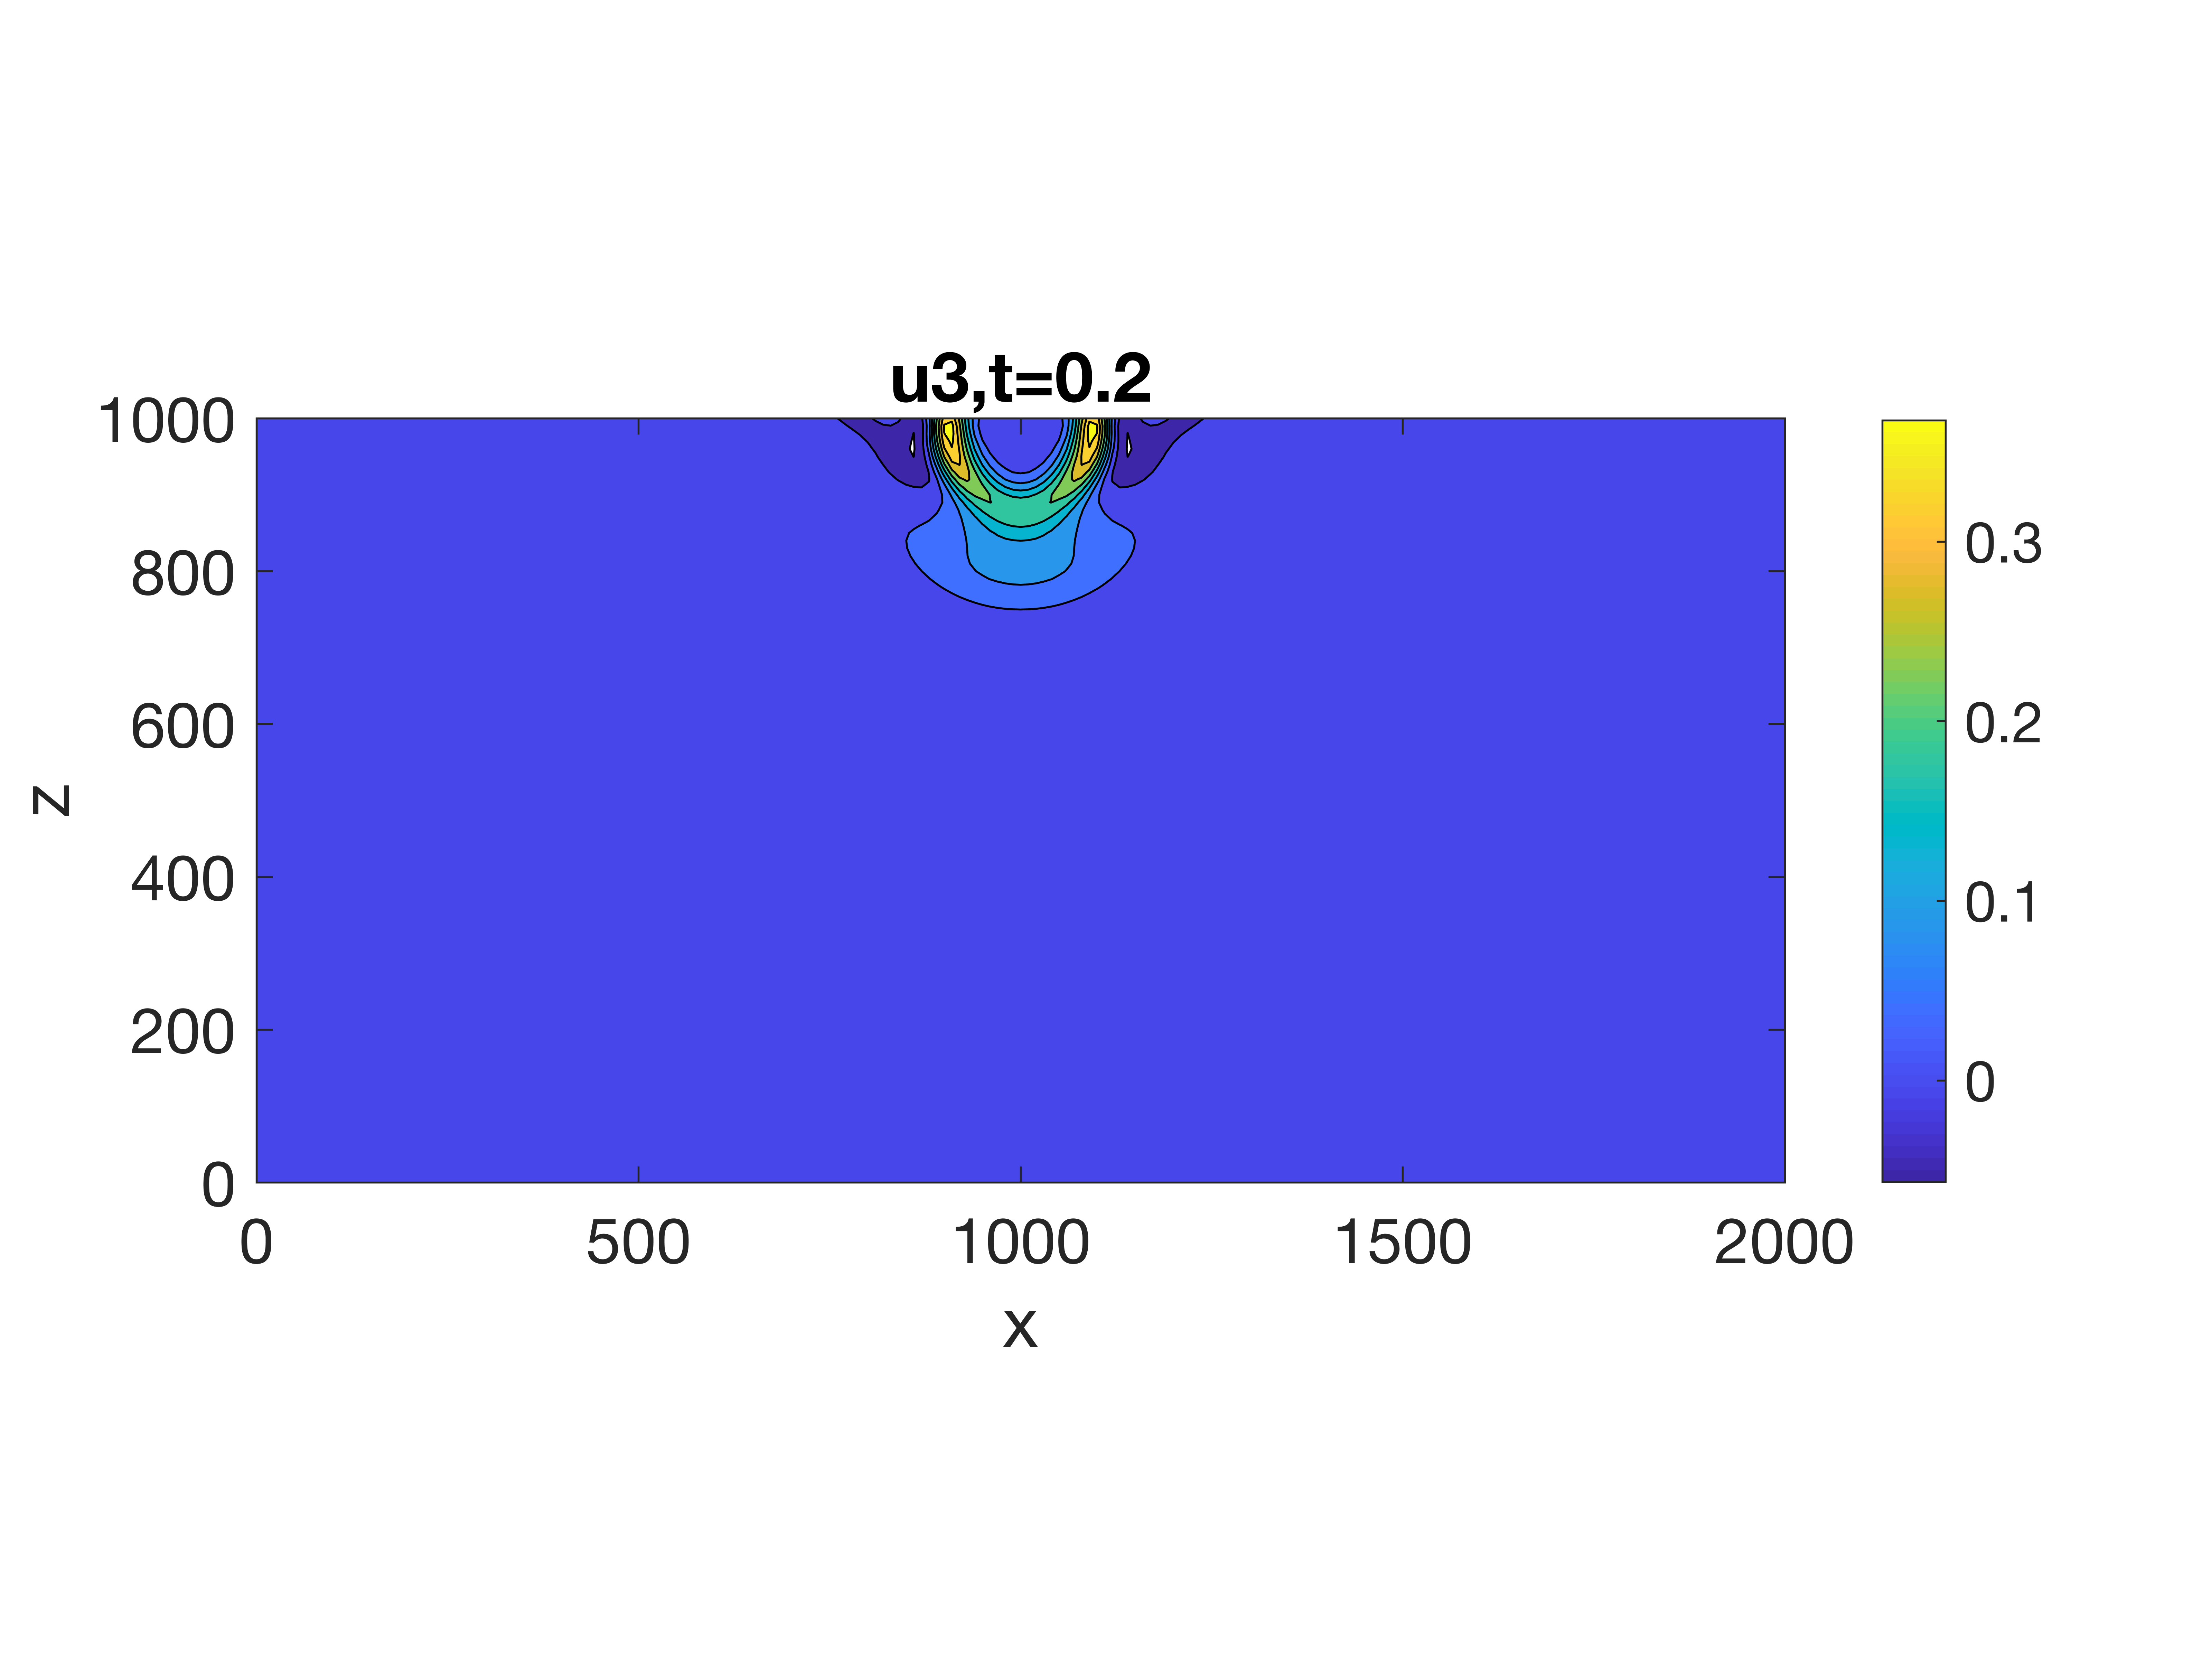
\includegraphics[width=0.45\textwidth]{u3_t02_cartesian.png}
	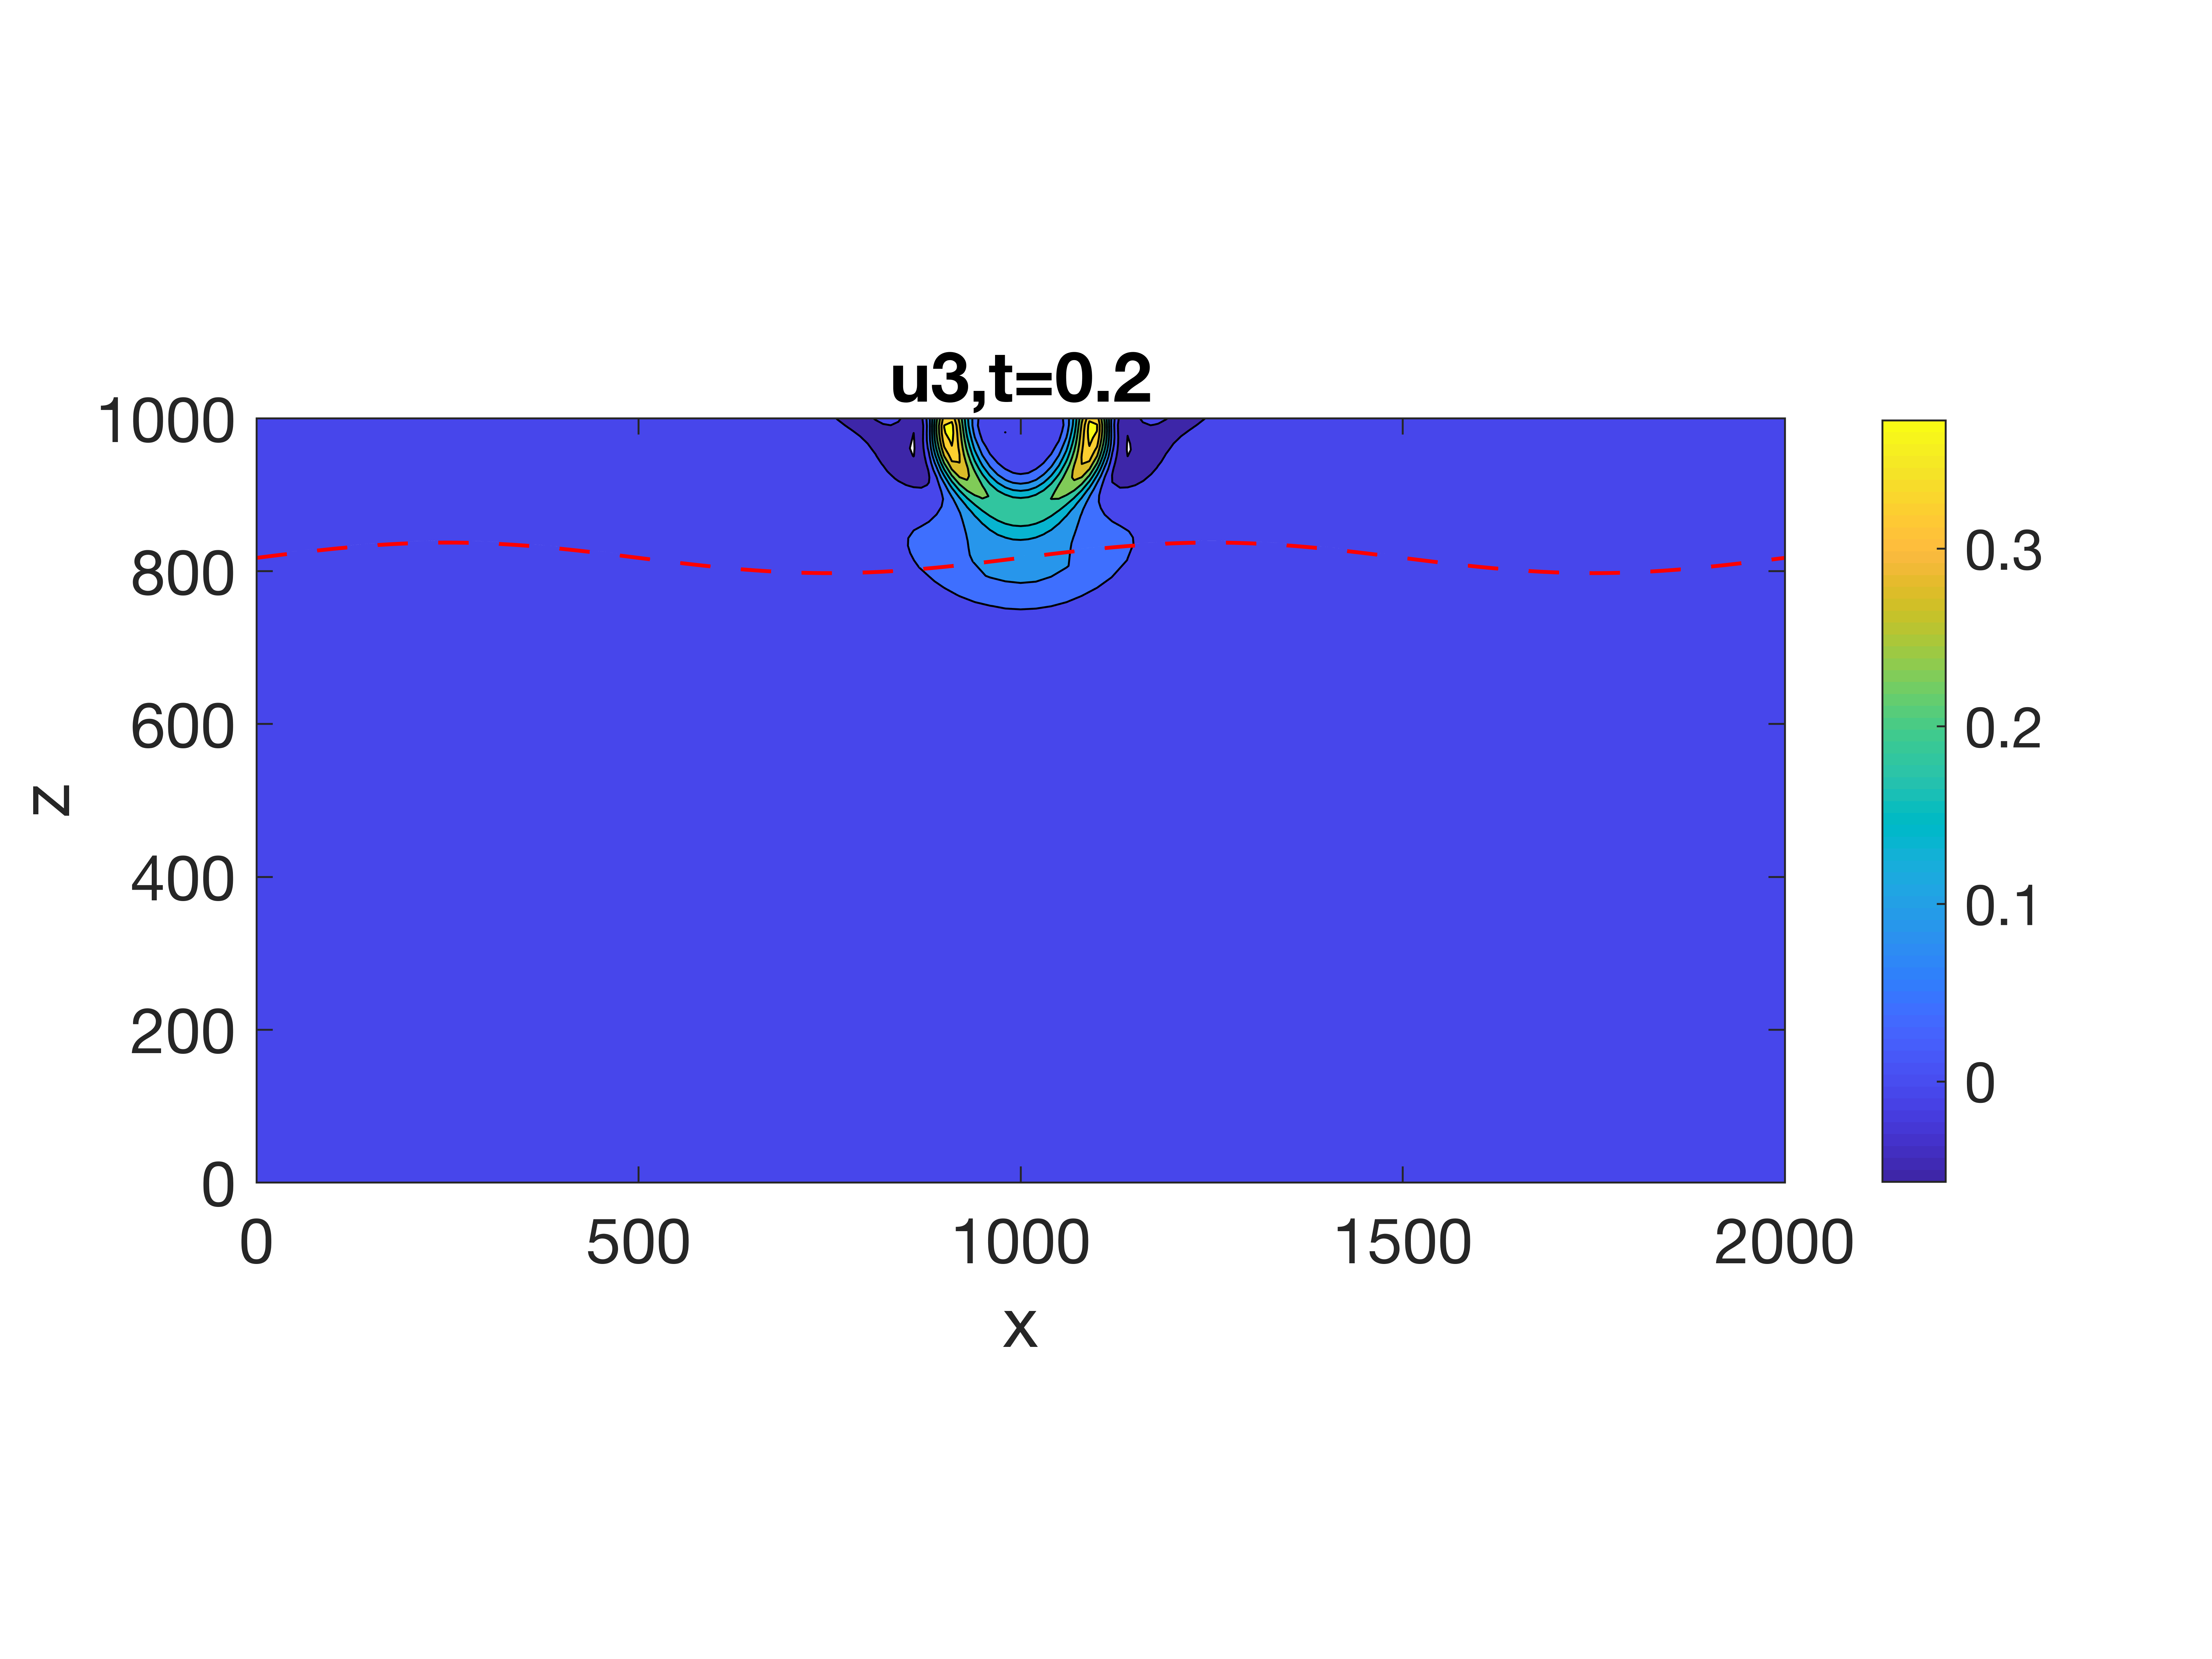
\includegraphics[width=0.45\textwidth]{u3_t02_curvi_mr.png}\\
	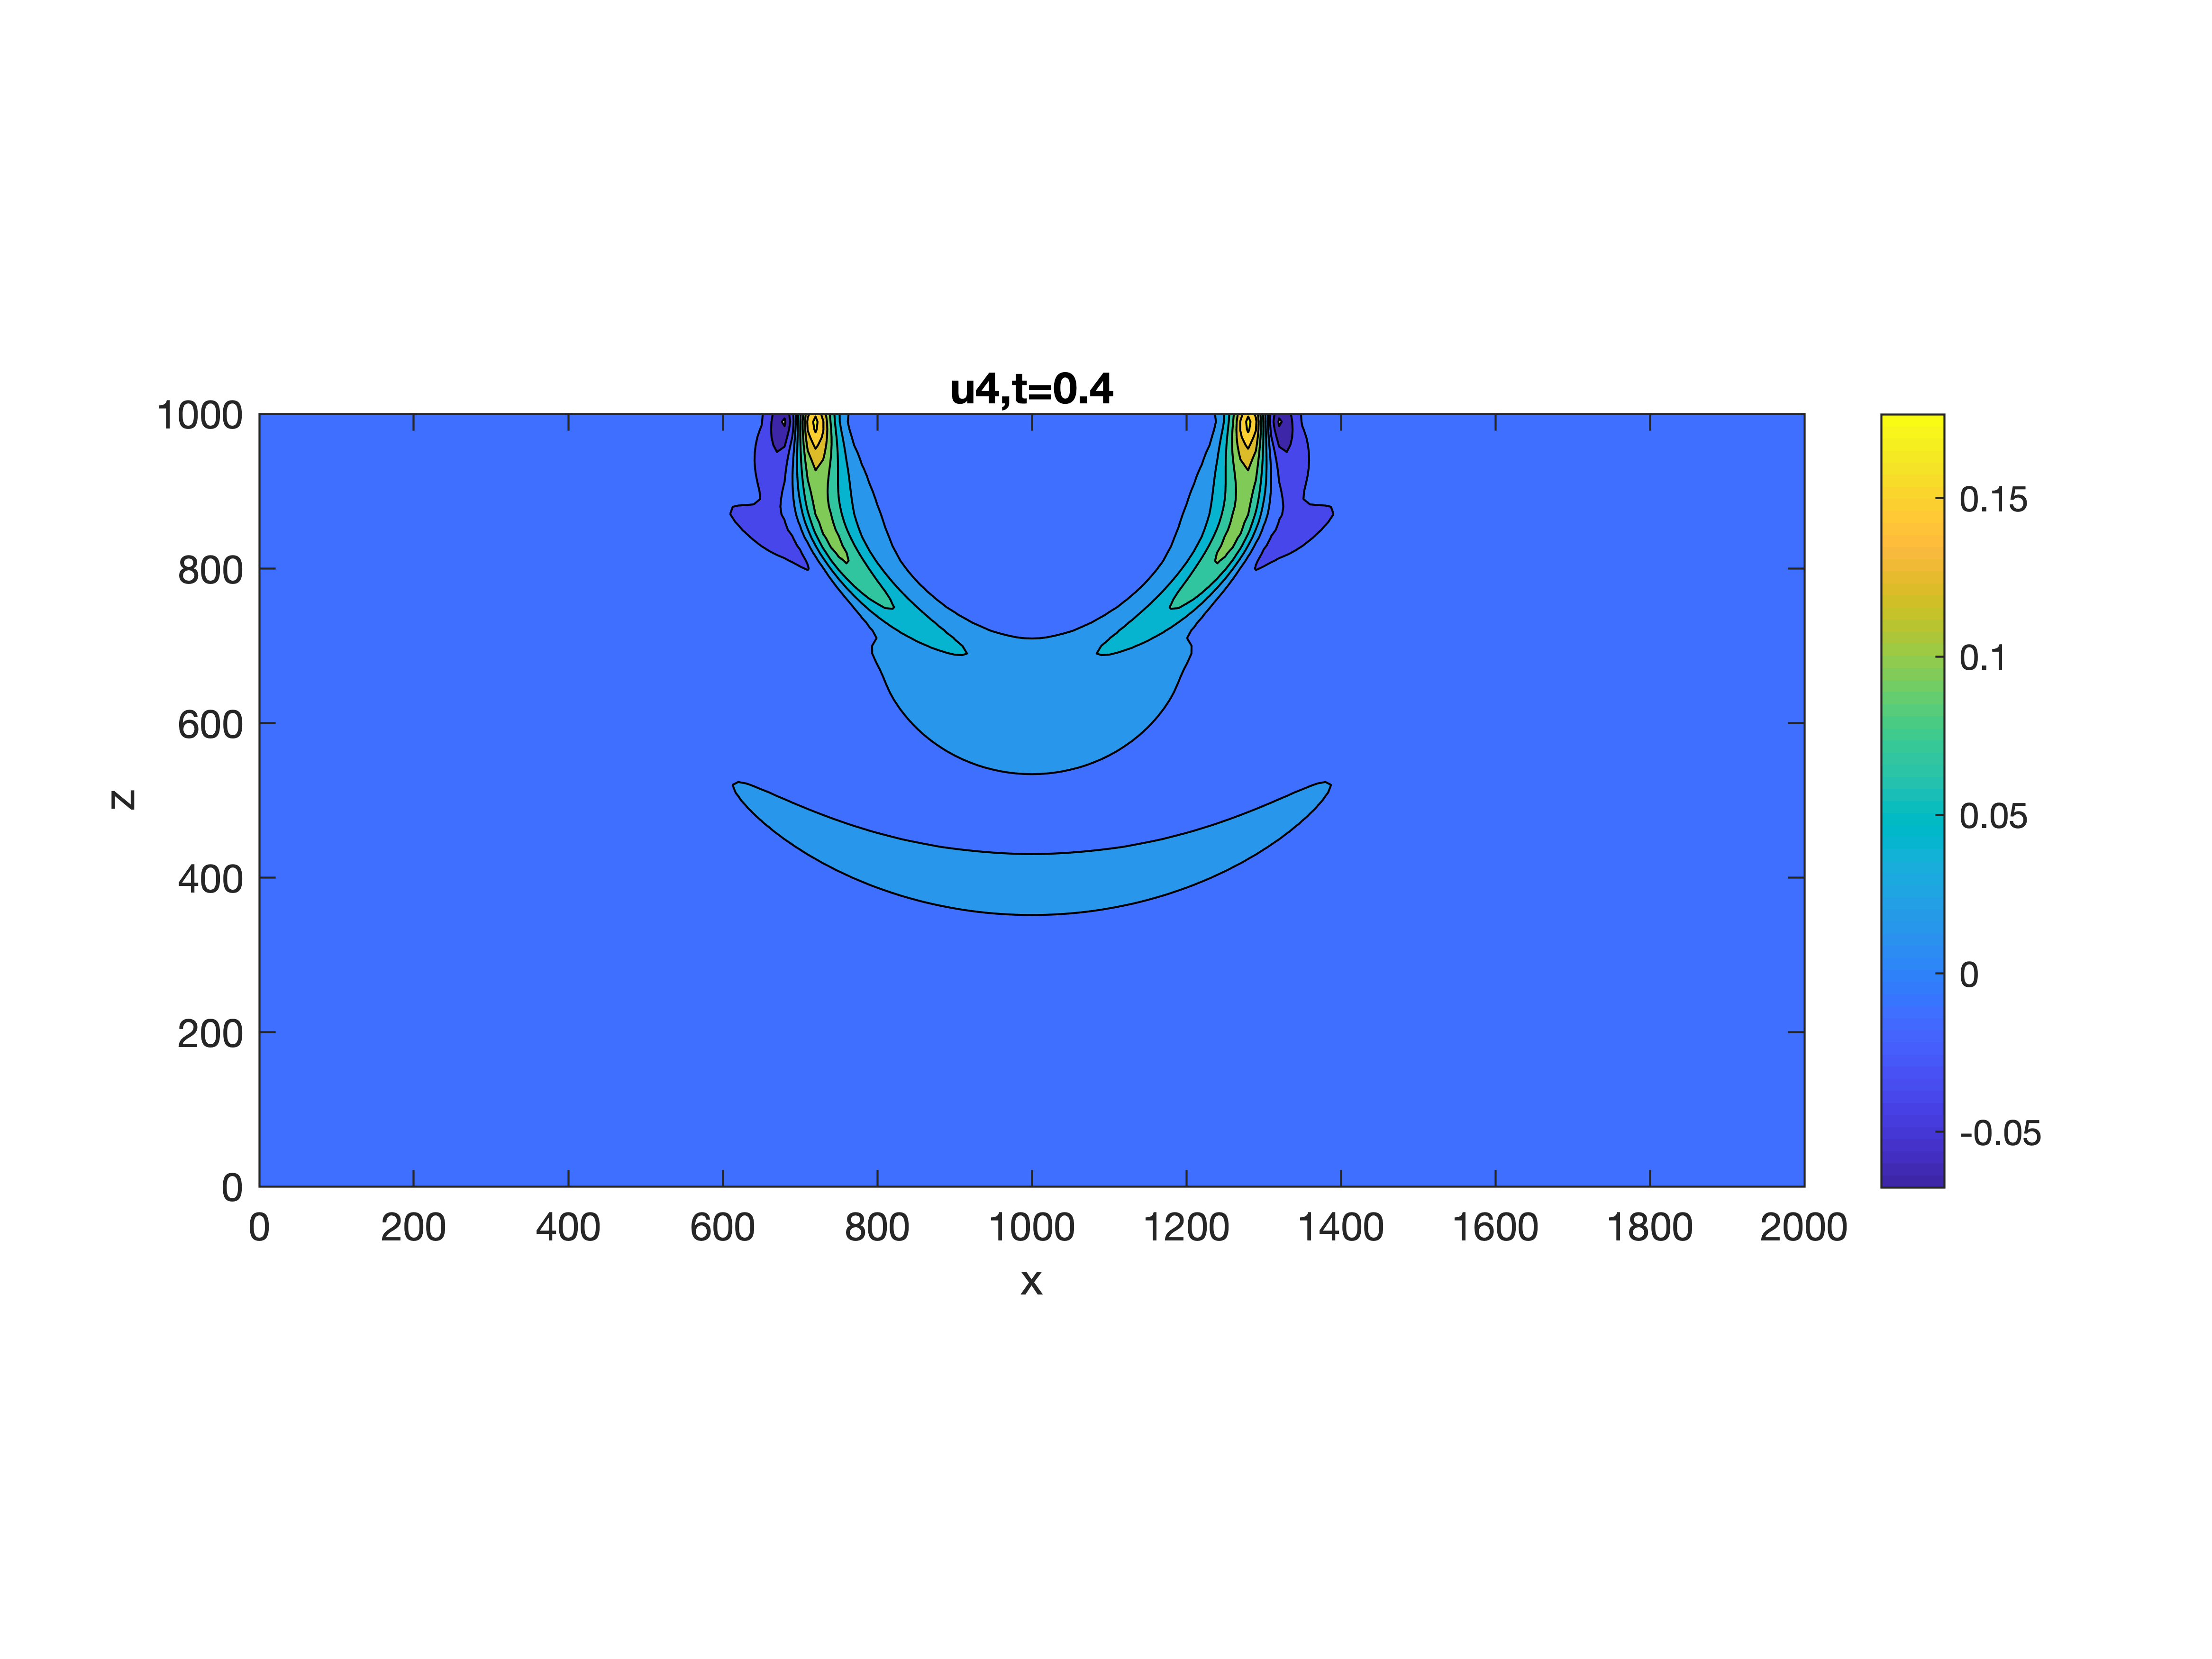
\includegraphics[width=0.45\textwidth]{u3_t04_cartesian.png}
	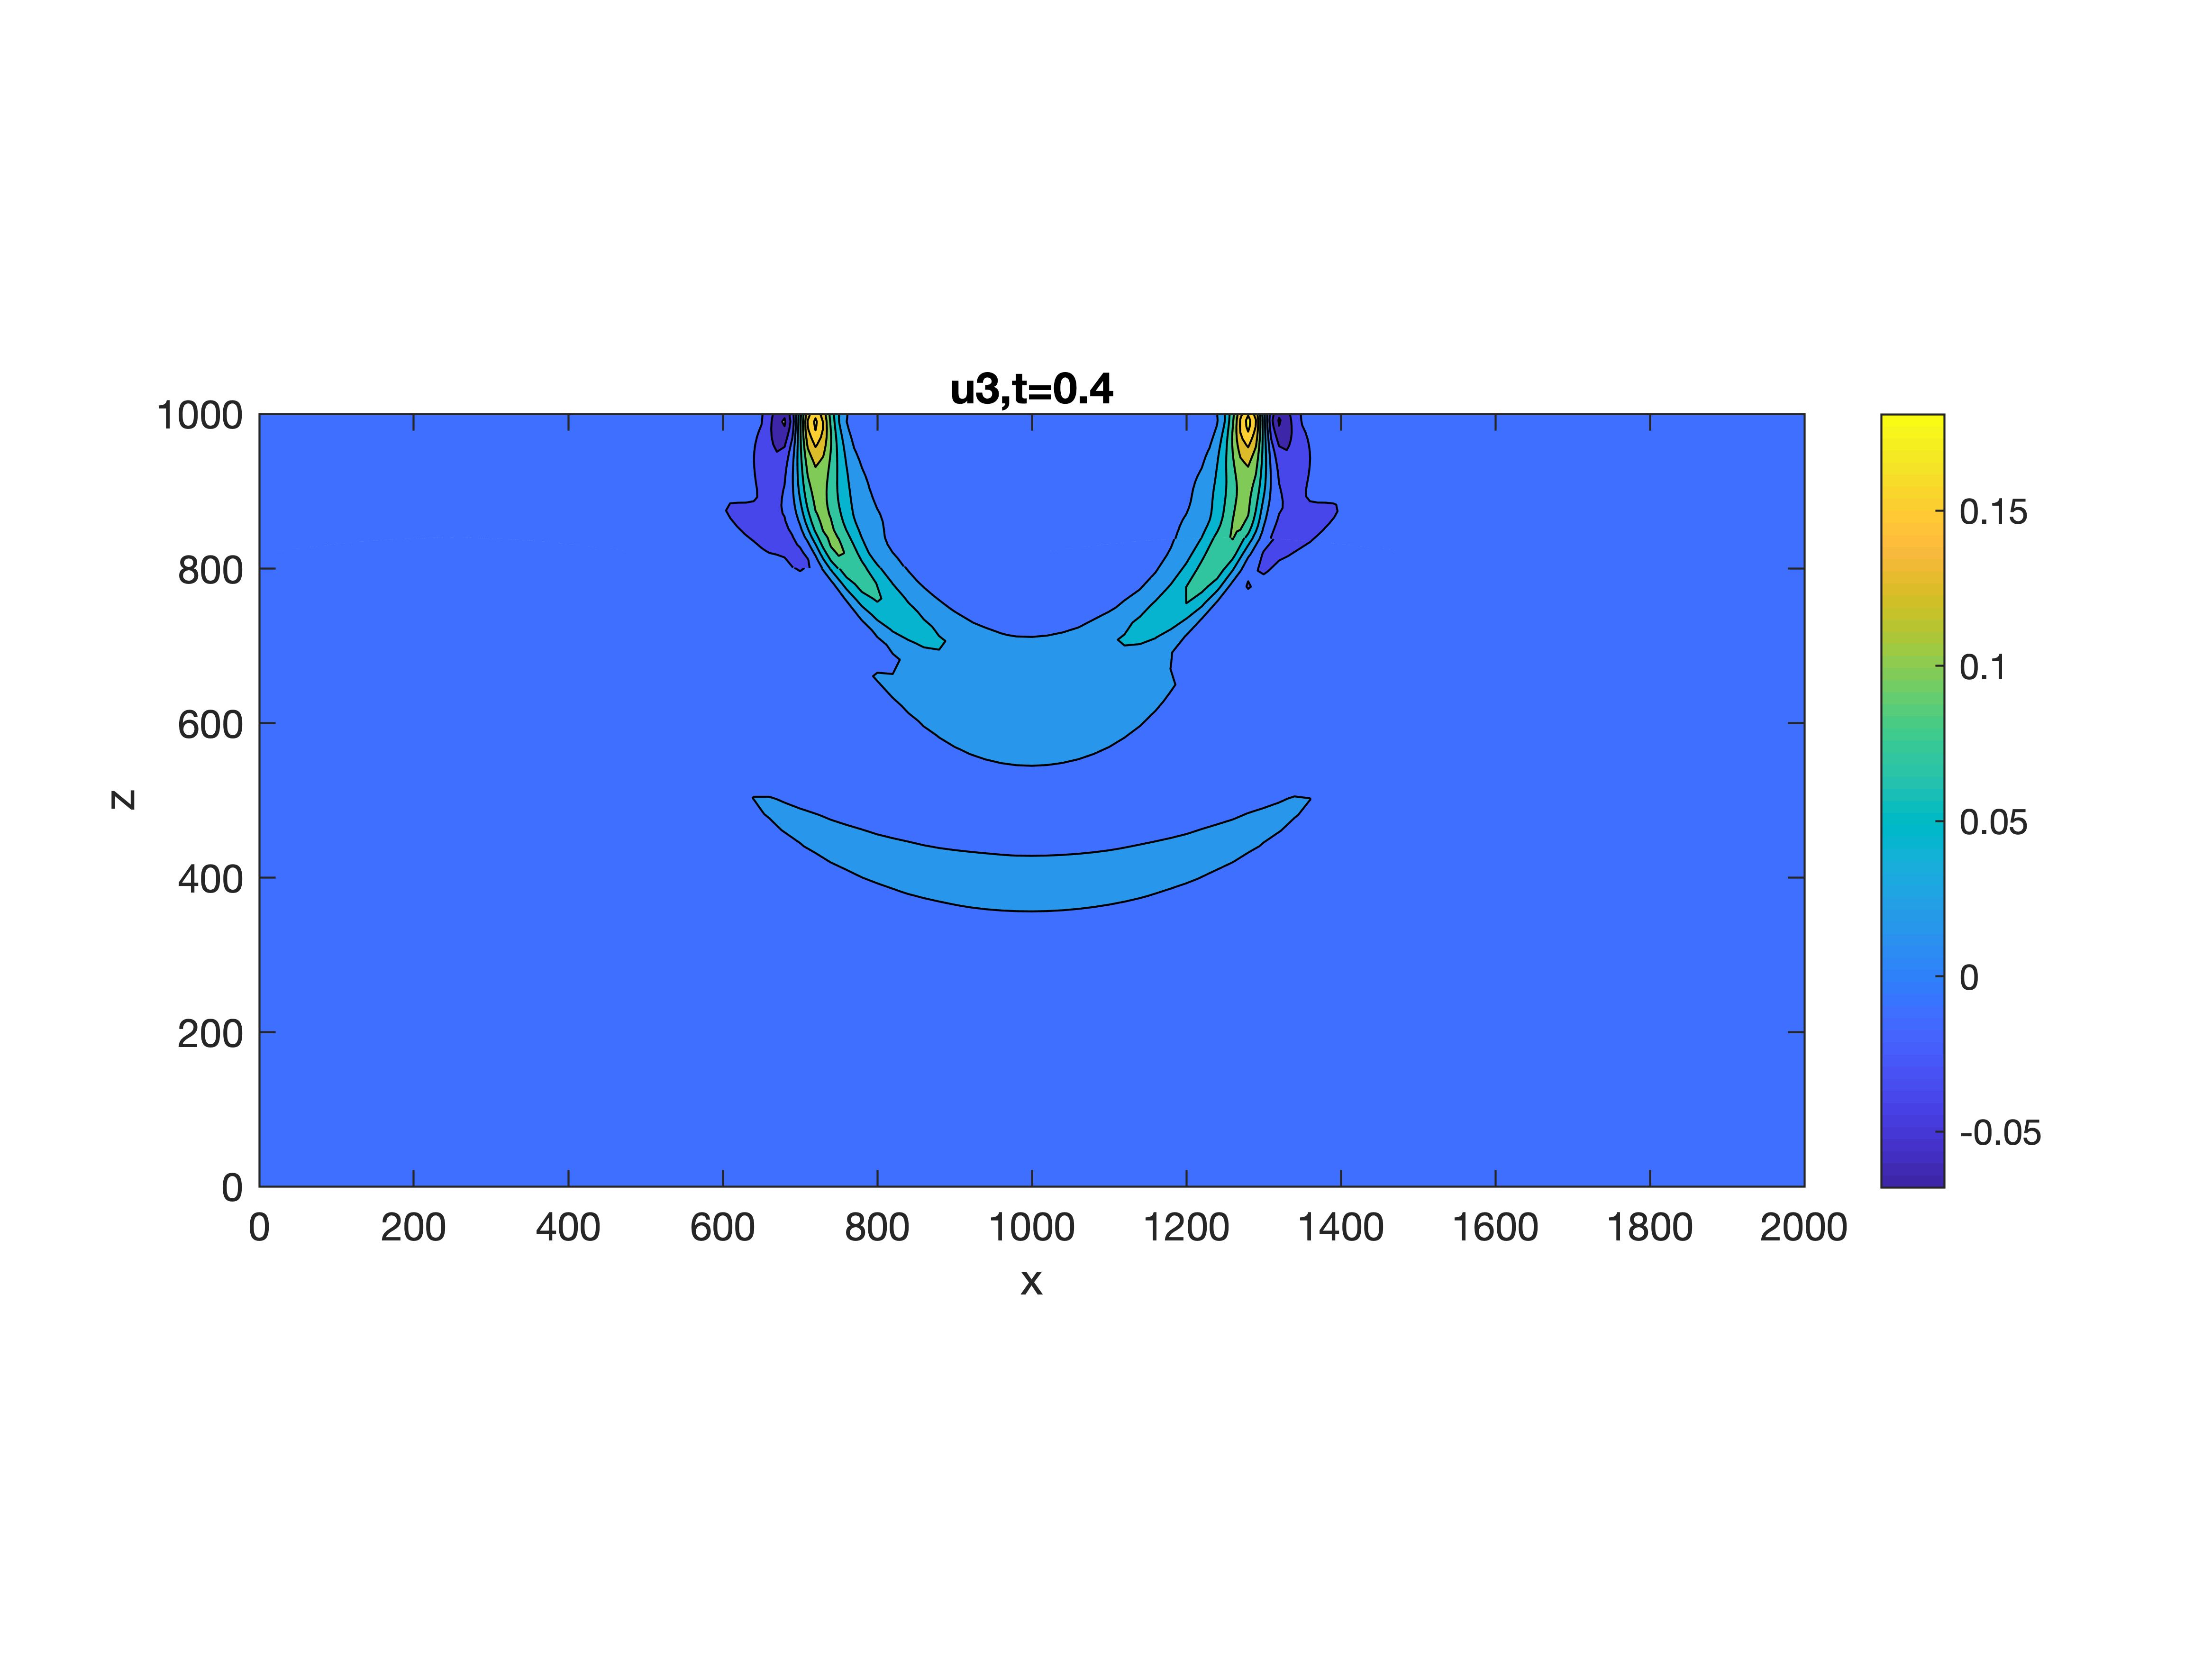
\includegraphics[width=0.45\textwidth]{u3_t04_curvi_mr.png}
	\caption{\scriptsize{The graph for $u_3$. From left to right are for Cartesian mesh without mesh refinement and curvi-linear mesh with mesh refinement respectively. From top to bottom are for $t = 0.2$ and $t = 0.4$ respectively.}}\label{u3}
\end{figure}
From Figure \ref{u1}, Figure \ref{u2} and Figure \ref{u3}, we observe that there is no significant reflection at the mesh refinement interfaces.

\subsection{Energy conservation test}\label{conserved_energy}
We shall have an experiment for energy conservation. We also need to evaluate the iterative methods. These can be Experiment 3, or incoporated in the first two experiments.

\section{Conclusion}
\end{document}
